\documentclass[12pt,upcase]{mitthesis}
\usepackage{amsmath}
%\newcommand{\angstrom}{\textup{\AA}}
\usepackage{microtype}
\usepackage{graphicx}
\graphicspath{{./images/}}
%\usepackage{multirow}
\usepackage{rotating}
\usepackage{natbib}
\usepackage{url}
\usepackage{booktabs}
\usepackage{makecell}
\usepackage{graphicx, float}            % Graphics/Images.
\usepackage{pgfplots, tikz}             % Drawing/graphing tools.
\usetikzlibrary{
    calc,                   % Calculating right angles and more.
    angles,                 % Drawing angles within triangles.
    arrows.meta,            % Latex and Stealth arrows.
    quotes,                 % Adding labels to angles.
    positioning,            % Relative positioning of nodes.
    decorations.markings,   % Adding arrows in the middle of a line.
    patterns,
    arrows,
    shapes,
    shapes.geometric,
    cd,
    hobby,
    babel
}                                       % Libraries for tikz.
\pgfplotsset{compat=1.9}                % Version of pgfplots.
\usepackage[]{pdfpages}
% for line numbers comment the next two lines before final submission
\usepackage{lineno}
\linenumbers*[1]
% use fancyhdr, to enable page style stuff (below)
\usepackage{fancyhdr}
\setlength{\headheight}{15.2pt}
\renewcommand{\headrulewidth}{0pt}

\pagestyle{plain}
\usepackage{import}                     % Import external files.
\usepackage[subpreambles=false]{standalone}      % Complileable sub files.
\begin{document}
%% Sherman 1
% Revision 1.1  92/04/22  13:08:20  epeisach

% BE SURE TO READ THE UNIVERSITY'S RULES ON WHAT FIELDS ARE REQUIRED OR ENCOURANGED FOR YOUR DEPARTMENT

\title{Remote sensing of the upper atmosphere using ground based imaging spectrograph}

\author{Saurav Aryal}

\prevdegrees{B.S., Winona State University (2009)}
\prevdegrees{M.Sc., Central Michigan University (2011)}

\department{Department of Physics and Applied Physics}

% If the thesis is for two degrees simultaneously, list them both
% separated by \and like this:
% \degree{Doctor of Philosophy \and Master of Science}
\degree{Doctorate}
\degreemonth{December}
\degreeyear{2018}
\thesisdate{December 1, 2018}

% If there is more than one supervisor, use the \supervisor command
% once for each.
\supervisor{Supriya Chakrabarti}{Associate Professor}
%\reader{Michelle Scribner-MacLean}{Assistant Professor} % reader is not necessary

% this is the department committee chairman, not the thesis committee chairman. 
\chairman{Robert Giles}{Department Chairman}

% Make the titlepage based on the above information.  If you need
% something special and can't use the standard form, you can specify
% the exact text of the titlepage yourself.  Put it in a titlepage
% environment and leave blank lines where you want vertical space.
% The spaces will be adjusted to fill the entire page.  The dotted
% lines for the signatures are made with the \signature command.
\maketitle

% The abstractpage environment sets up everything on the page except
% the text itself.  The title and other header material are put at the
% top of the page, and the supervisors are listed at the bottom.  A
% new page is begun both before and after.  Of course, an abstract may
% be more than one page itself.  If you need more control over the
% format of the page, you can use the abstract environment, which puts
% the word "Abstract" at the beginning and single spaces its text.

%% You can either \input (*not* \include) your abstract file, or you can put
%% the text of the abstract directly between the \begin{abstractpage} and
%% \end{abstractpage} commands.

% First copy: start a new page, and save the page number.
\newpage
\thispagestyle{empty}
\mbox{}
\newpage
\thispagestyle{empty}

% Second copy: start a new page, and reset the page number.  This way,
% the second copy of the abstract is not counted as separate pages.
\pagestyle{plain}
\newpage
\setcounter{page}{1}
\pagenumbering{roman}
\begin{abstractpage}
% sherman 1
% $Log: abstract.tex,v $
% Revision 1.1  93/05/14  14:56:25  starflt
% Initial revision
% 
% Revision 1.1  90/05/04  10:41:01  lwvanels
% Initial revision
% 
%
%% The text of your abstract and nothing else (other than comments) goes here.
%% It will be single-spaced and the rest of the text that is supposed to go on
%% the abstract page will be generated by the abstractpage environment.  This
%% file should be \input (not \include 'd) from cover.tex.

Complex processes in the upper-atmosphere of the Earth give rise to optical emissions in the form of airglow and aurora. Thus, these emissions are key diagnostics to study the processes involved in the upper-atmosphere. Simultaneous observations of these emissions allows one to (a) determine the characteristics of the precipitating particles that produced the aurora, (b) infer changes in the upper atmosphere and the photochemical processes leading to these emissions. A versatile new ground-based spectrograph known as High-Throughput and Multislit Imaging Spectrograph (HiT\&MIS) has been developed to observe airglow and auroral emissions simultaneously at six selected wavelengths on a round-the-clock basis. The selected spectral features are: HI 656.3 nm, HI 486.1 nm, OI 557.7 nm, OI 630.0 nm, OI 777.4 nm and $N_2$$^+$ 427.8 nm. The brightnesses of these emission features change simultaneously but differently depending on the energy of the precipitating electrons, the density structure of the atmospheric constituents producing these emissions and the mechanisms of how particular emissions are produced. Hence, these simultaneous measurements can be utilized to infer the energy characteristics of the precipitating electrons. For the current dissertation, (i) the characteristic energy and energy flux of energetic electron precipitation were inferred based on simultaneous measurements of OI 557.7 nm, OI 630.0 nm and $N_2$$^+$ 427.8 nm emission features during an auroral events. Measurement of these optical emissions were modeled based on an electron transport and chemical reaction model, in terms of atmospheric composition, geophysical parameters and the energy and energy flux of the precipitating particles.The method presented in this dissertation provides a way multispectral imagers can be used as a stand-alone tool to derive energy and energy flux during auroral events. In addition, (ii) because each airglow emission occurs at a particular altitude, round-the-clock measurement of multiple airglow emission features will be used to trace changes in the upper atmosphere at different altitudes. The proposed study will allow us to observe the solar-terrestrial interactions from the ground at high temporal resolution during both geomagnetically quiet and active times.
\end{abstractpage}

%%%%%%%%%%%%%%%%%%%%%%%%%%%%%%%%%%%%%%%%%%%%%%%%%%%%%%%%%%%%%%%%%%%%%%
% -*-latex-*-




%% !TEX root = Thesis.tex
% put this as first line (commented) of every file

\begin{titlepage}
\begin{center}
\vspace*{1cm}

{\Large Title}

\vspace{1.5cm}

BY

\vspace{1.5cm}

SAURAV ARYAL\\
B.S. UNIVERSITY OF WHEREVER (May 2009)\\
M.S. UNIVERSITY OF WHEREVER ELSE (December 2011)

\vfill

SUBMITTED IN PARTIAL FULFILLMENT OF THE REQUIREMENTS\\
FOR THE DEGREE OF DOCTORATE OF PHILOSOPHY\\
DEPARTMENT OF PHYSICS AND APPLIED PHYSICS\\
UNIVERSITY OF MASSACHUSETTS LOWELL

\vfill

\end{center}

\noindent\begin{tabular}{ll}
\makebox[4in]{} & \makebox[1.5in]{}\\
\makebox[4in]{\hrulefill} & \makebox[1.5in]{\hrulefill}\\
Author: Your Name & Date\\[4ex]
\end{tabular}

\noindent\begin{tabular}{l}
\makebox[5.7in]{\hrulefill}\\
Thesis Advisor: Dr. Supriya Chakrabarti \\[4ex]
\makebox[5.7in]{\hrulefill}\\
Committee Member: Dr. Timothy Cook \\[4ex]
\makebox[5.7in]{\hrulefill}\\
Committee Member: Dr. Andryi Danylov
\end{tabular}
\end{titlepage}

%\chapter*{Acknowledgments}
\renewcommand{\thefootnote}{\fnsymbol{footnote}}

Acknowledge those who helped you. I offer no comment on proper degree of mushiness. The work in this thesis was only possible because of all the helpful and guiding members of the UMass Lowell engineering education community. Many people have helped me not just in research effort, but in introducing me to new thoughts and ideas that became foundational to this project.

This material is based upon work supported by the National Science Foundation under Grants No. DRL-0000000 and No. DGE-0000000.\footnote{Any opinions, findings, and conclusions or recommendations expressed in this material are those of the author and do not necessarily reflect the views of the National Science Foundation.}

\renewcommand{\thefootnote}{\arabic{footnote}} % Puts footnotes back to numeric mode for the rest of the document

% -*- Mode:TeX -*-
%% This file simply contains the commands that actually generate the table of
%% contents and lists of figures and tables.  You can omit any or all of
%% these files by simply taking out the appropriate command.  For more
%% information on these files, see appendix C.3.3 of the LaTeX manual. 
\tableofcontents
\newpage
\listoffigures
\newpage
\listoftables

%\chapter*{Preface}
The preface is not part of the thesis standard, but is optionally available if you find it prudent. Uncomment it in main.tex.
 	% Preface is not part of the standard. I invented it for myself. Use it if you want by uncommenting.

	% Redefine the "plain" pagestyle to have pagenum in the header, right
	\fancypagestyle{plain}{
		\fancyhf{}
		\fancyhead[R]{\thepage}
	}

	\setcounter{page}{1}
	\pagenumbering{arabic}
	\pagestyle{plain}
	
% \chapter{Introduction}
% The upper atmosphere of the earth (90 km+, defined in section \ref{sec:str}) is influenced by forcing from below (the lower atmosphere) as well as forcing from above (the sun). The upper atmosphere is in a weak plasma state due to ionization of chemical species by high energy solar radiation. Understanding the processes in the upper atmosphere thus is important. In this thesis, we study the upper atmosphere during two phenomenon: one involving particle entry and the other involving dynamics generated by thermal changes.
\section{Dissertation Outline}

This thesis is focused on observing the Thermosphere-Ionosphere (TI) system, which lies in the earth's upper atmosphere, using a ground-based multi-spectral imager known as High Throughput \& Multi Slit imaging Spectrometer (HiT\&MIS). Based on observations, two different phenomenon are studied. The first phenomena involves estimation of the energitics of solar particle entry during an auroral event. The second phenomena involves temperature changes in the upper atmosphere that leads to waves. In this chapter, first, background on the earth's atmosphere and the TI system is given; then, information on how the observation is tied to the TI system is provided. In chapter 2, details on different instruments that were used for this thesis is provided. Chapter 3 describes methods created to simultaneously derive the energy and flux of electrons penetrating into the atmosphere based on multi-spectral imaging of auroras. Chapter 4 presents characterization of Traveling Ionospheric Disturbances (TIDs) generated by Atmospheric Gravity Wave (AGWs) observed using multiple instruments including HiT\&MIS.

This dissertation contains modified versions of the publications "Derivation of the energy and flux morphology in an aurora observed at mid‐latitude using multi‐spectral imaging"  by \citep{aryal} and "Multi-spectral and multi-instrument observation of TIDs following the Total Solar Eclipse of August 21, 2017" by Aryal et al b. [in review].


\section{Structure of the Atmosphere}
\label{sec:str}
Earth’s atmosphere can be divided into many different layers based on the temperature profile, how the chemical species mix and the differences in dominant physical processes and so on. In terms of the temperature profile, the Earth’s atmosphere is divided into: 
\begin{itemize}
	\item The troposphere (0 -15 km in altitude), where temperature decreases with altitude due to decrease in infrared radiation from the Earth. 
	\item The stratosphere (15-50 km), where there is an increase in temperature as UV radiation is absorbed by ozone, the mesosphere (50-90 km) where the temperature decreases due to radiative cooling.
	\item The thermosphere (90-600 km), where the temperature increases rapidly due to absorption of high energy solar radiation.  High energy solar radiation also ionize chemical (neutral) species in the thermosphere creating the ionosphere.
\end{itemize}
In terms of mixing, the Earth’s atmosphere is divided into two regions. 
\begin{itemize}
	\item The heterosphere (up to 100 km) is where all the chemical species are well-mixed due to turbulence. 
	\item The homosphere ($>$ 100 km) is where chemical species are not well-mixed due to diffusion and the density structure of each species is determined by mass. That is, the lighter chemical species are found higher in the atmosphere.  
\end{itemize}
In terms of differences in dominant physical processes, the Earth’s atmosphere is divided into 
\begin{itemize}
	\item the lower atmosphere (0-15 km), 
	\item the middle atmosphere (15-90 km) and 
	\item the upper atmosphere (90 km and above). 
\end{itemize}

\begin{figure}[t]
	\centering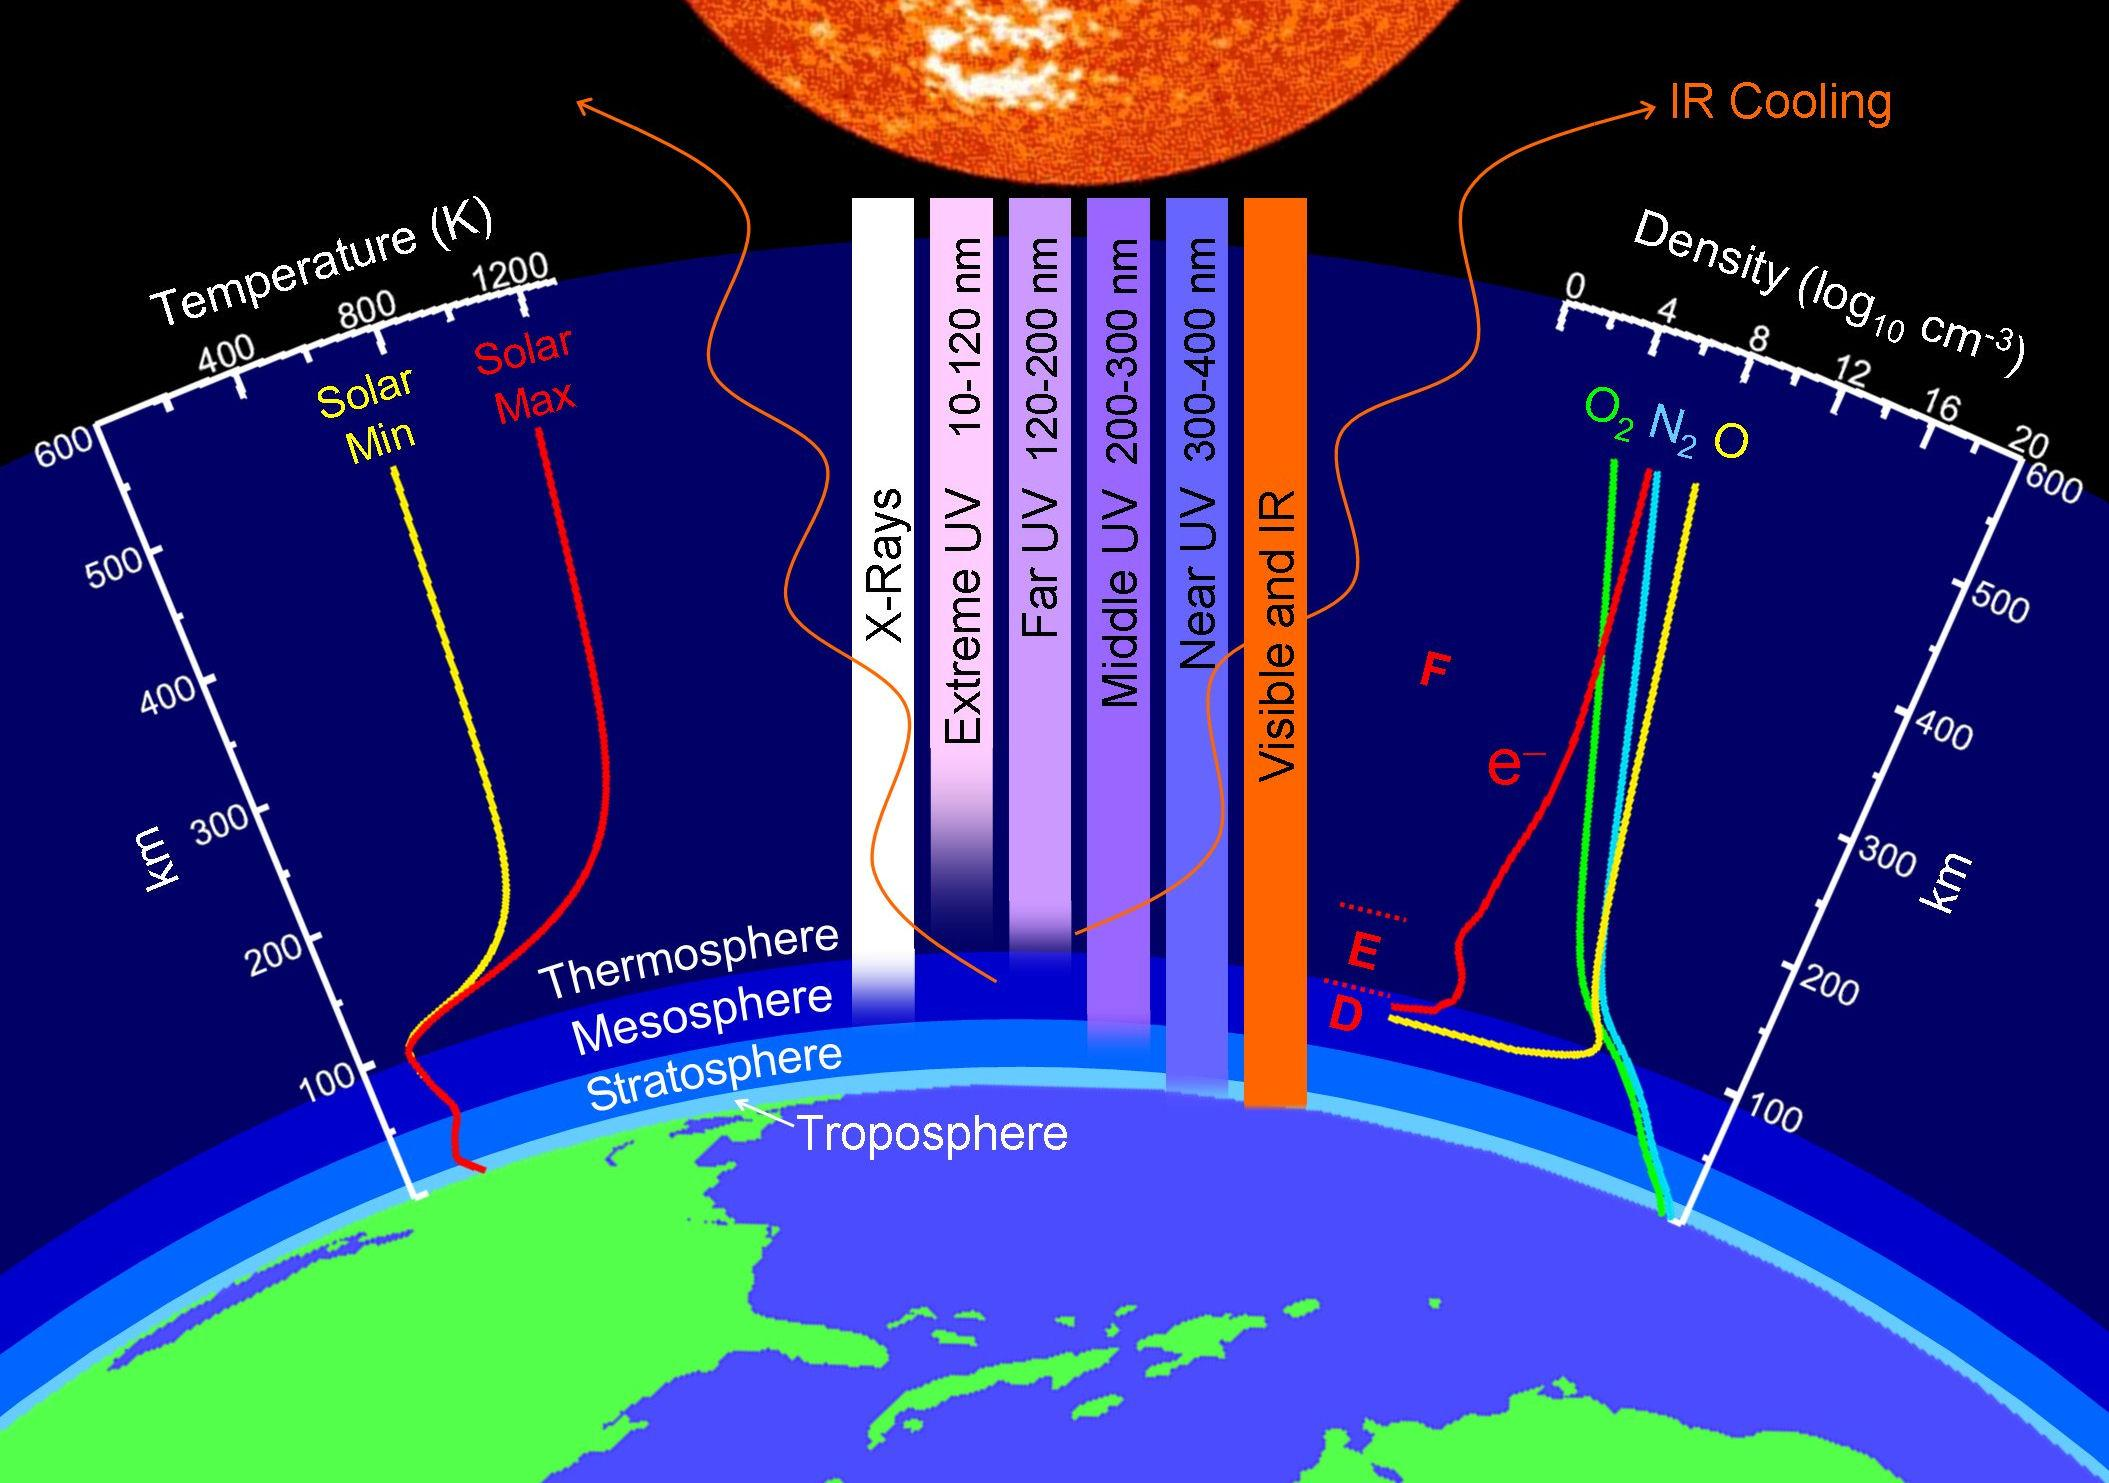
\includegraphics[width=32pc]{vert_stu.jpg}
	\caption{Vertical structure of the Earth's atmosphere in terms of temperature, density of chemical species and where solar radiation at different wavelengths get absorbed. Source: John Emmert, NRL}
	\label{fig:vert_str}
\end{figure}

%%%%


\section{Theory of the Planetary Atmosphere}
In 1D geometry (put a simple figure) the pressure (p) gradient can be written as:
\begin{equation}
\label{eq:he}
\frac{dp}{dz} = -g(z) \rho
\end{equation}
which comes from applying Newton's second law to small parcel of gas with density ~$\rho$ contained in height, dz. Assuming ideal gas, we can write the pressure (p) as $\frac{\rho}{M}$ k T, where k is the Boltzmann's constant, T is the temperature, and M is the molecular mass of the gas. Replacing the pressure (p), and assuming p and T not function of height (z), equation \ref{eq:he} becomes:
\begin{equation*}
\frac{dp}{dz}= -p \frac{M g}{k T} = -\frac{p}{H}  \\
\end{equation*}
\begin{equation*}
\implies \frac{dp}{p}=-\frac{dz}{H}
\end{equation*}
\begin{equation}
\label{eq:p}
\implies p (z)= p(z_{0}) e^{-\frac{z-z_{0}}{H}} \implies n(z)= n(z_{0}) e^{-\frac{z-z_{0}}{H}} 
\end{equation}
where, H = $\frac{k T}{M g}$ is known as the scale height, z$_0$ is the reference height and n is the number density. The scale height, H, is the height at which the pressure (and the number density) drops by $\frac{1}{e}$.  For the heterosphere, i.e. the well mixed atmosphere < 100 km, M is the mean molecular weight of all the atmospheric species. Above $\rm \sim$100 km (homosphere), the chemical species diffusively separate and each chemical species follow their own scale height, H$_i$= $\rm \frac{k T}{M_{i} g}$ ; where H$_i$ and M$_i$ are the scale height and the molecular mass of the i$^{\rm th}$ atmospheric species.

So far we have assumed that the temperature and the gravity are constant with respect to the atmospheric height. This is an ideal over-simplification, the gravity drops smoothly with height and the temperature changes differently at different layers of the atmosphere (see Section \ref{str}). There are also various chemical and physical processes that transport atmospheric constituents and break hydrostatic equilibrium. Thus, in general the atmosphere is sliced into thin layers where T and g are assumed to be constant. 
\begin{figure}[t]
	\centering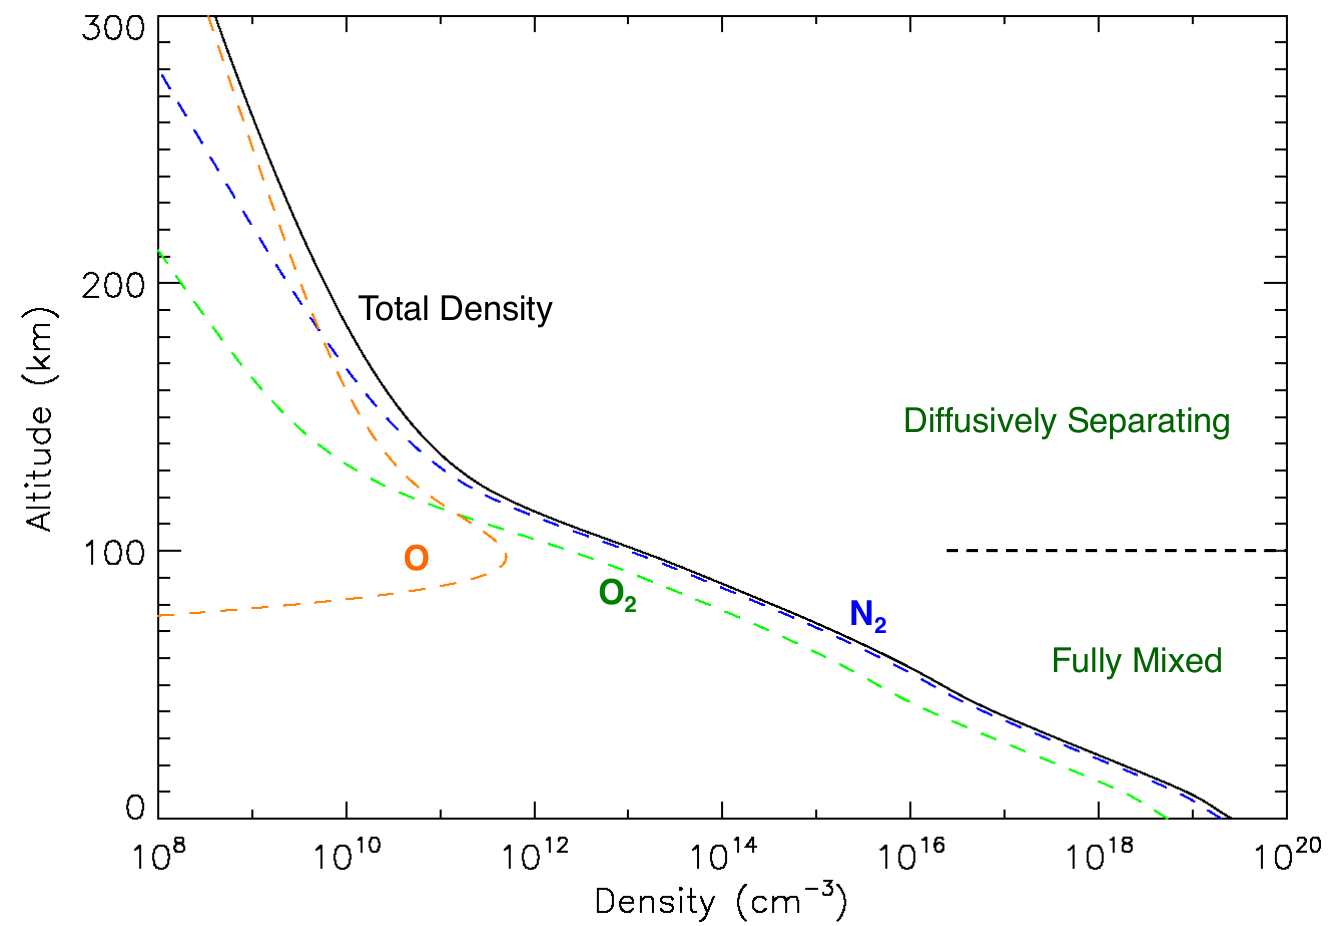
\includegraphics[width=35pc]{ok_dens_str_neu.png}
	\caption{Neutral density structure of the Earth's atmosphere. Plot courtesy Dr. Stan Solomon, NCAR}
	\label{fig:neu_den}
\end{figure}
\section{Upper Atmosphere}
The upper atmosphere is the first to receive the radiative energy input (dominant in mid and low latitudes) and in the form of charged particle input (dominant in higher latitudes) from the Sun. The high energy solar radiation (X-rays and UV) have an ionizing effect on the constituents present in the upper atmosphere, thus creating the ionosphere, the ionized part of the upper atmosphere. This the upper atmosphere is a mixture of neutral, ionized chemical species and electrons whose interactions are then affected by the presence of the Earth’s magnetic field. This thesis is focused on the remote sensing of the upper-atmosphere and specifically the thermosphere and the ionosphere (embedded within the thermosphere).

\section{Thermosphere and Ionosphere}

The upper-atmosphere is the first to receive energy inputs from the sun in form of radiation and energetic particles. In the mean time, the density of neutral gases decrease exponentially with altitude and such that the density is space-like. The high energy solar inputs and low neutral density gives rise to a favorable environment in ionizing the atoms and molecules (also dissociate molecules) creating a space like plasma environment. Furthermore, absorption of high energy solar radiation leads to heating and the temperature rises rapidly with altitude and then plateaus creating the thermosphere. Together with the charged portion of the upper atmosphere, i.e. the ionosphere, this part of the upper atmosphere is known as the Thermosphere-Ionosphere (TI).
%%%Solar spectrum
\begin{figure}[t]
	\centering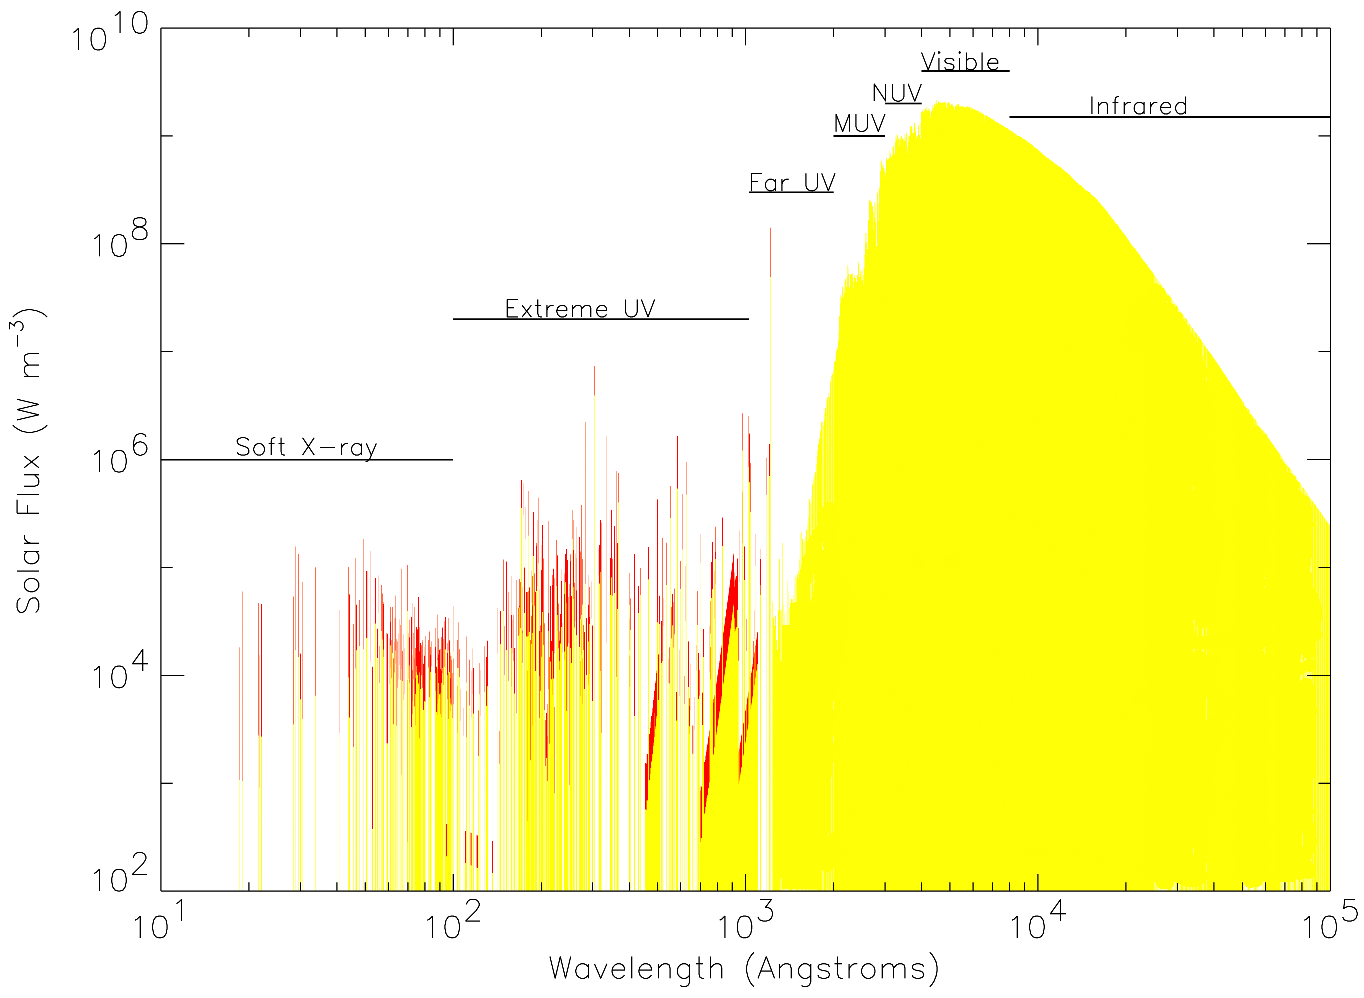
\includegraphics[width=35pc]{solar_spec.png}
	\caption{Typical example of solar spectrum incident on top of the Earth's atmosphere. Notice that the high energy radiation (X-ray and UV) vary a lot while the visible and infrared spectrum do not change. Plot courtesy of Dr. Stan Solomon, NCAR }
	\label{fig:solar_spec}
\end{figure}
%%%%%% Absorbtion of solar radiation
\begin{figure}[t]
	\centering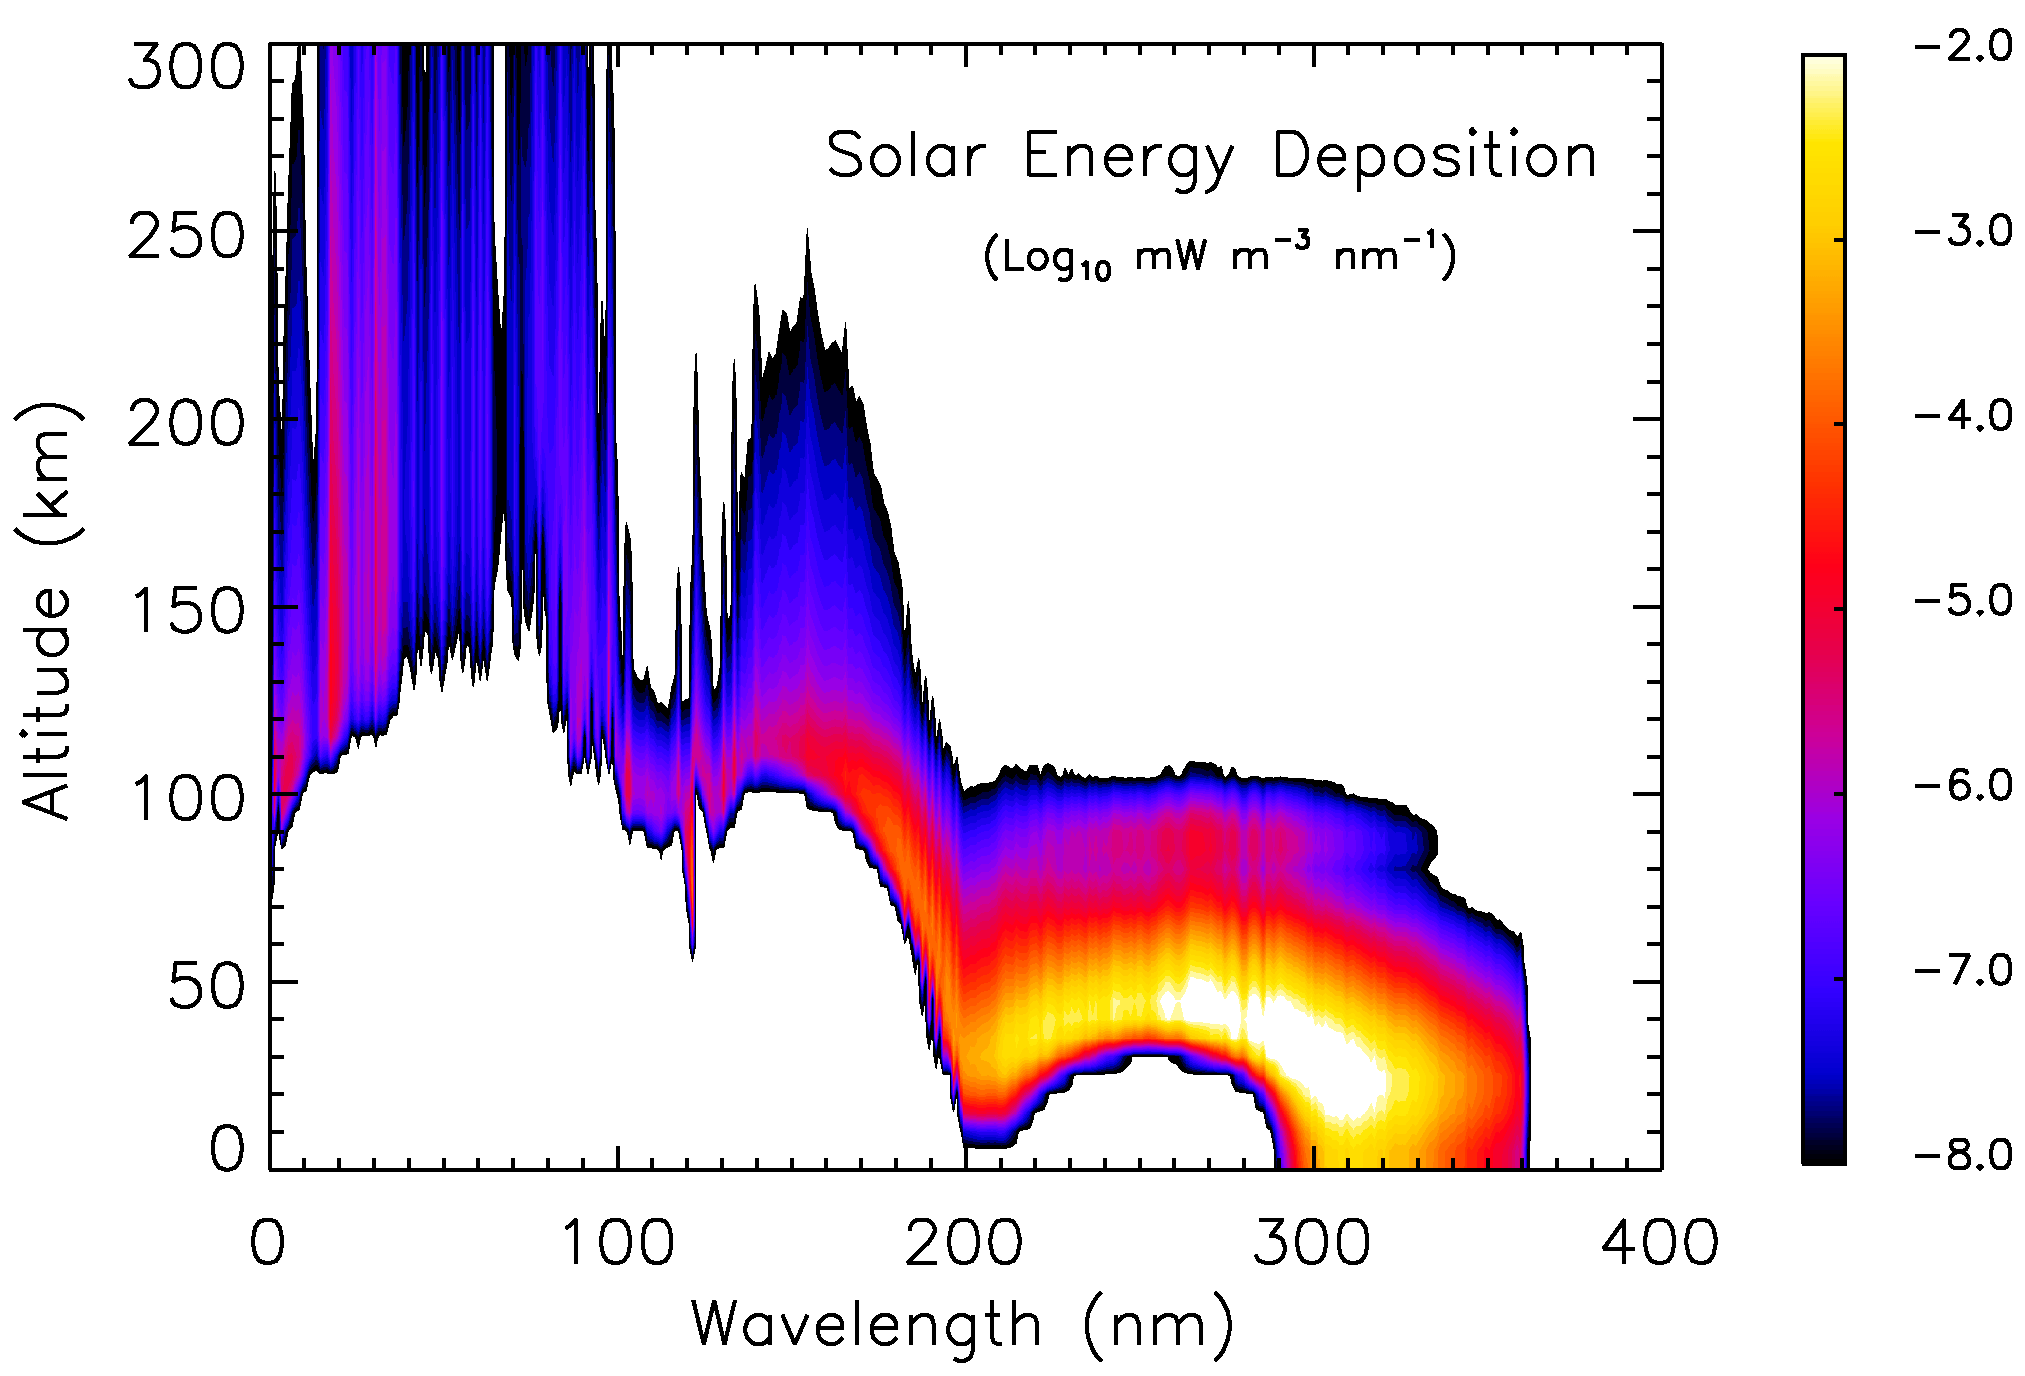
\includegraphics[width=35pc]{slr_rd_abs.png}
	\caption{Solar energy deposition in the Earth's atmosphere. Notice that most the highest energy radiation (< 200 nm) are absorbed before thy reach 100 km. Plot courtesy of Dr. Stan Solomon, NCAR }
	\label{fig:sl_rad_abs}
\end{figure}
%%%%temperature structure plot
\begin{figure}[t]
	\centering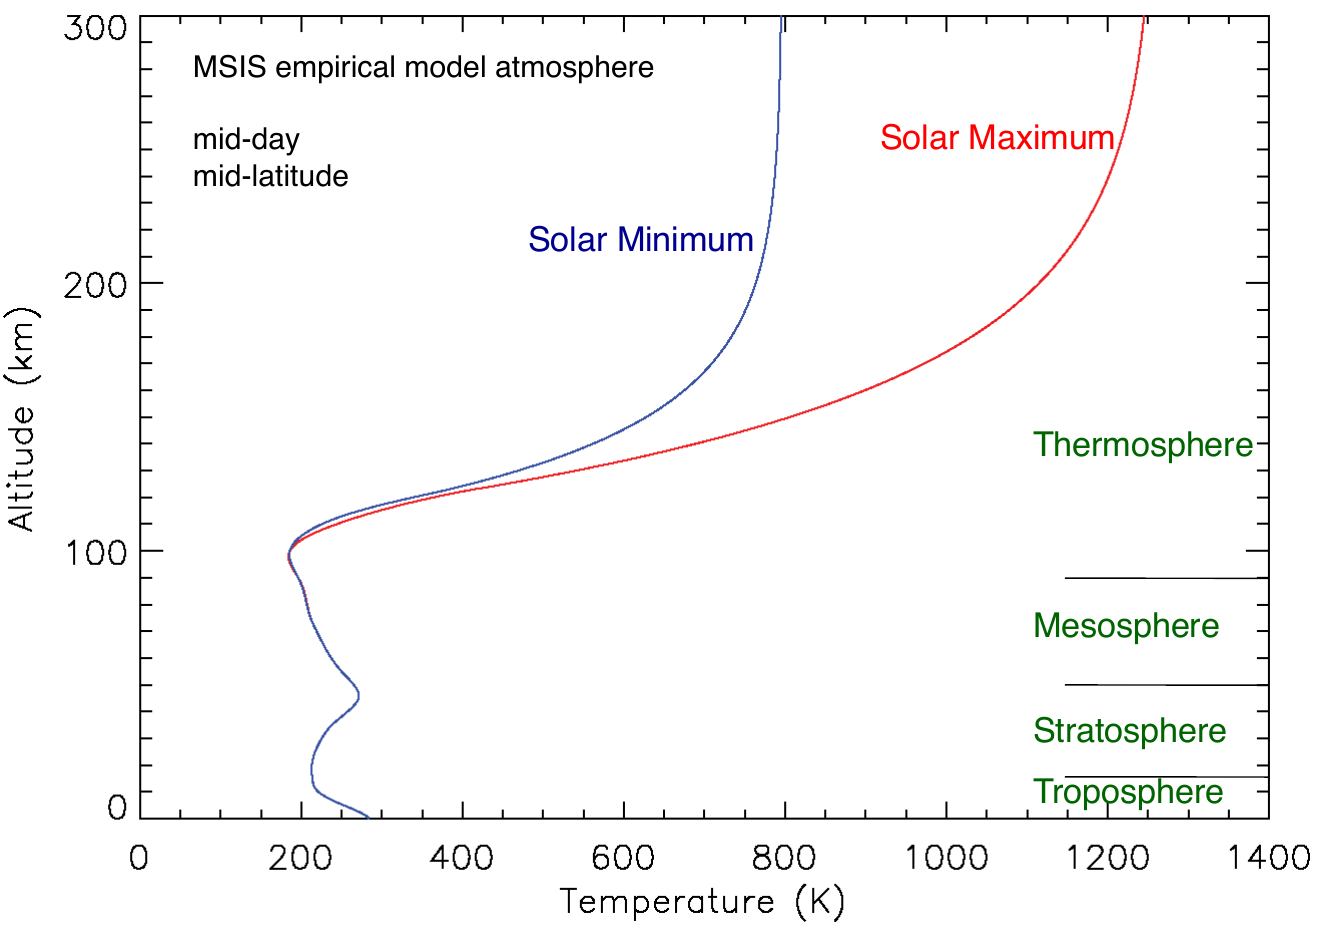
\includegraphics[width=35pc]{okl_temp_stru_slr_min_max.png}
	\caption{Temperature structure of the Earth's atmosphere based on MSIS. Notice sharp rise in temperature at the bottom of the Thermosphere which plateaus. Plot courtesy of Dr. Stan Solomon, NCAR }
	\label{fig:TI_temp_var}
\end{figure}
\begin{figure}[t]
	\centering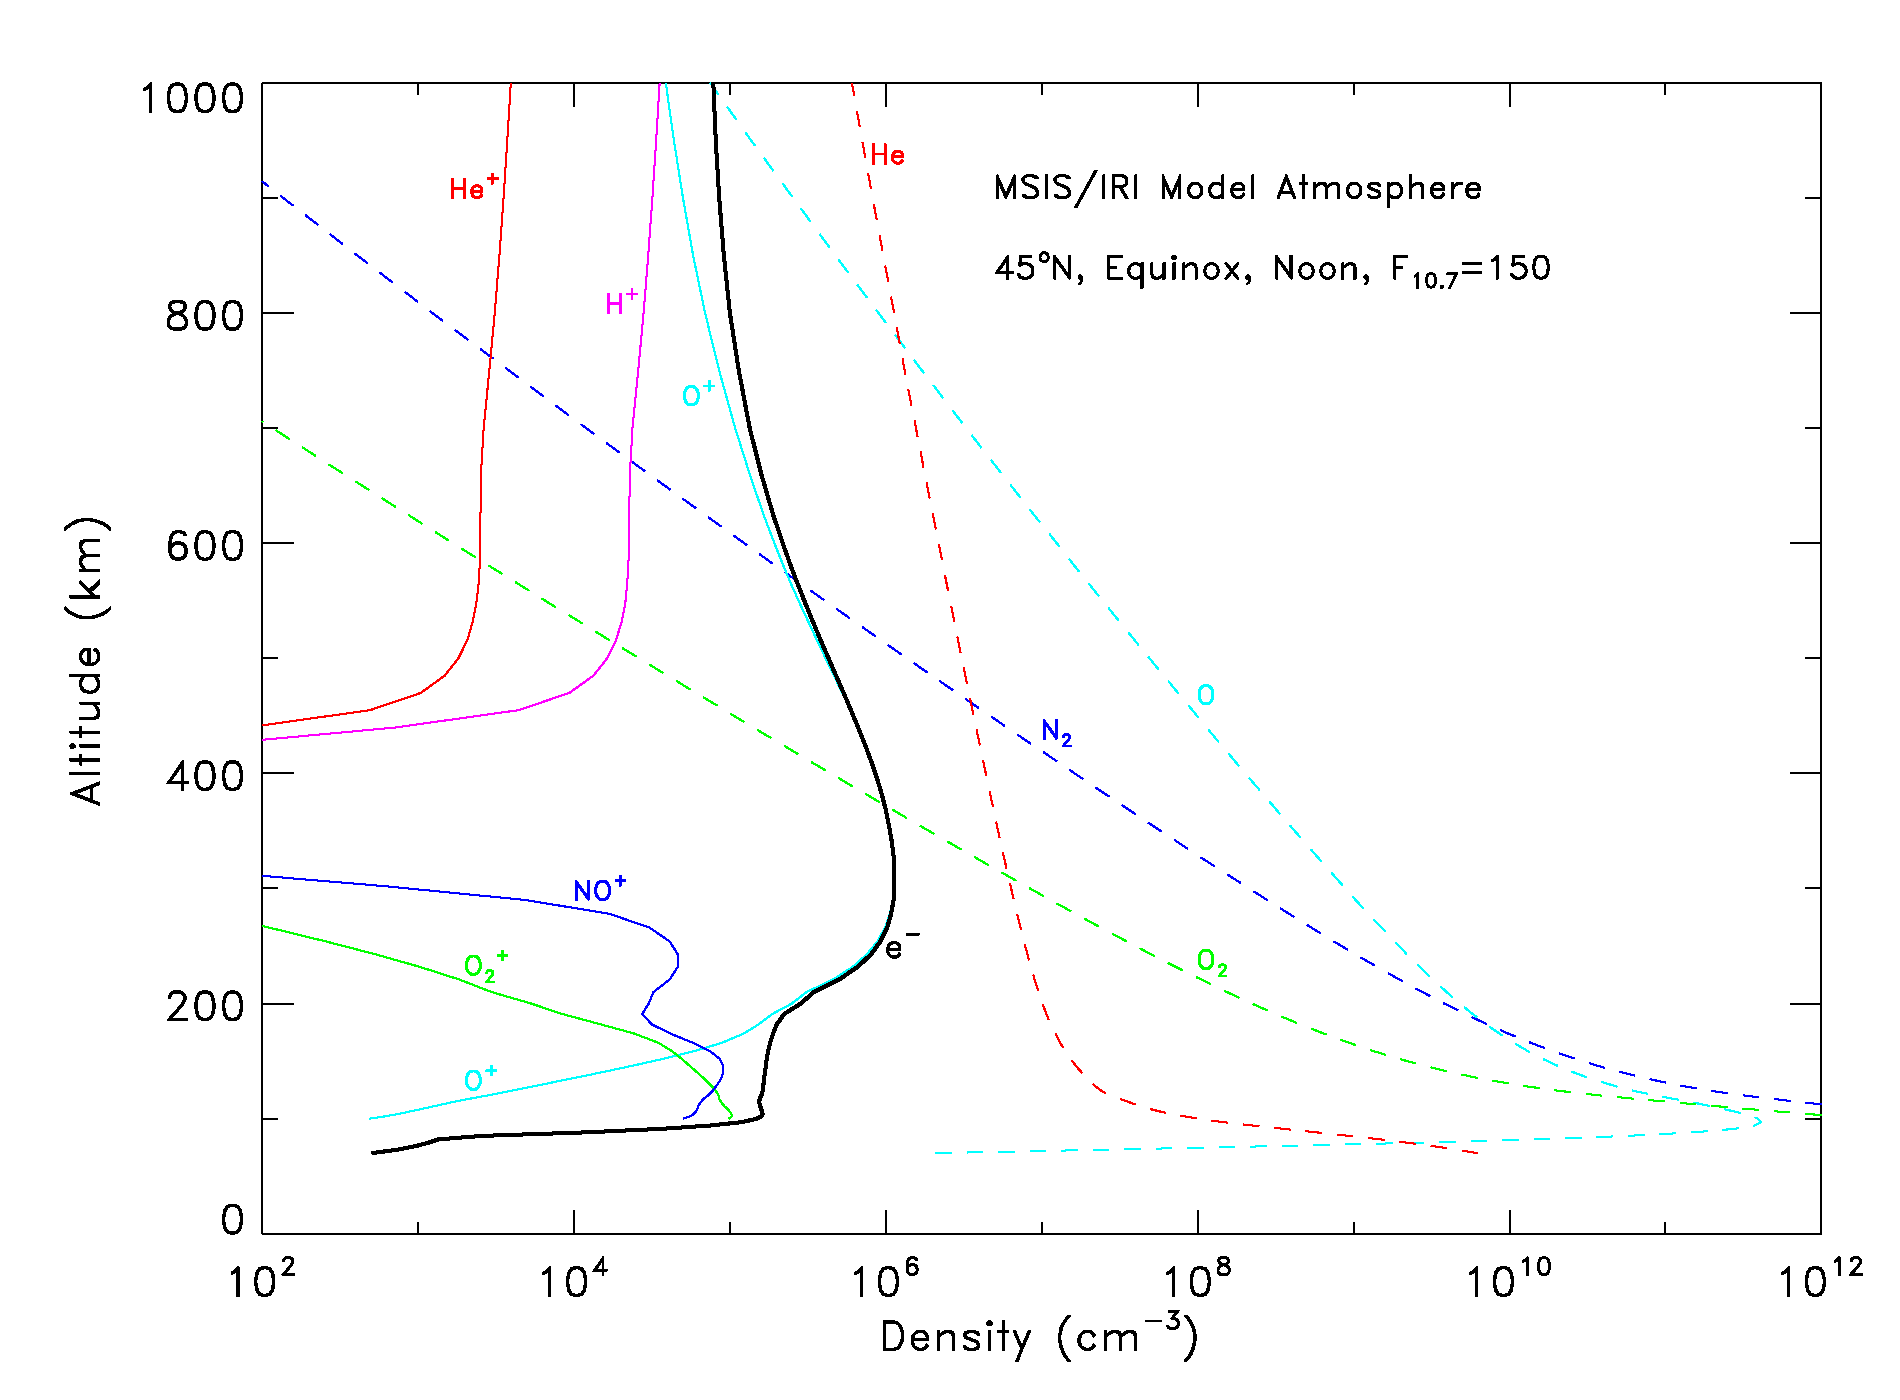
\includegraphics[width=35pc]{thm_dens.png}
	\caption{Density structure of neutral and ionic species in the Earth's atmosphere based on MSIS and IRI climatological models. Notice lighter atoms and ions are only present above $\rm \sim$ 100 km. Plot courtesy of Dr. Stan Solomon, NCAR }
	\label{fig:TI_dens}
\end{figure}
In the lower portions of the TI, the density of the neural species are high enough to get affected by the neutral dynamics (weather) at lower altitudes. Hence, the TI system is influenced by forcing from above (sun) and below (tropospheric weather). This making it an ideal laboratory to study the solar-terrestrial interaction.
\subsection{Ionosphere}
Ionization due to high energy solar radiation plus collisional ionization by energetic particles of the upper atmospheric constituents creates a weakly ionized region known as the ionosphere (about 80-1000 km).

\subsection{TI climatological Variability}
The climatological variability in the TI system is driven by the Solar Cycle. The solar cycle is the ... (put a image of solar cycle)
\begin{figure}[t]
	\centering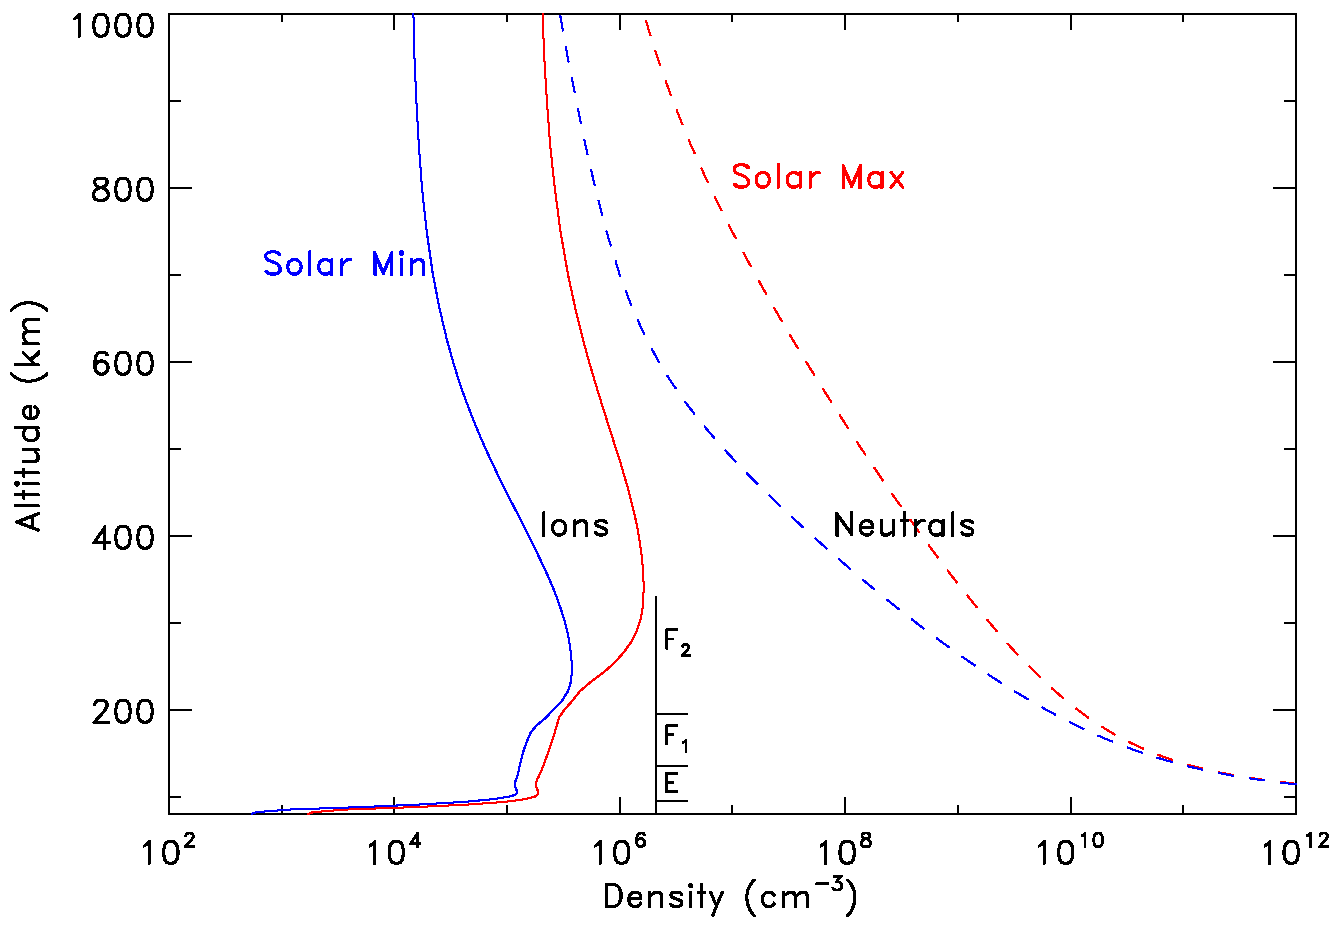
\includegraphics[width=35pc]{slr_minmax_slm.png}
	\caption{Density structure in the TI. Both ion and neutral density increase during the solar max period. Plot courtesy of Dr. Stan Solomon, NCAR }
	\label{fig:TI density variability}
\end{figure}


Thermosphere is also where most of the satellites, including the International Space Station (ISS) reside. So, studying the upper atmosphere also helps in quantifying the effects of upper-atmospheric weather (referred as space weather hereafter) on expensive satellites as well as health effects on Astronauts. In addition, different technologies based on satellites (GPS, satellite internet, etc.) could get disrupted by space weather. Like terrestrial weather, the long term goal for space weather is to predict adverse weather before hand to limit economic damage caused by such events.

\subsection{Solar inputs on the TI system}
The continuous stream of charged particles from the Sun (solar wind) with its embedded magnetic field, known as the Interplanetary Magnetic Field (IMF), hits the Earth and pushes and distorts the Earth’s magnetic field. This creates a long cigar-shaped region where charged particle motion is controlled by Earth’s magnetic field called the magnetosphere (see Fig. 1). Most of the energetic particles carried by the solar wind flow around this distorted magnetic field, except around the magnetic poles. Around the magnetic poles, the more perpendicular orientation of the Earth’s magnetic field allows more solar particles to enter the upper atmosphere of the Earth, either directly through the magnetic cusp (Fig. 1) or due to magnetic reconnection. In addition, there is a reservoir of trapped high energy charged particles around the Earth in regions known as the radiation belts (Fig. 1). These radiation-belt particles can diffuse or get accelerated into the upper atmosphere and interact with the upper atmosphere. Most of the entry of the energetic particles occurs at high latitudes; however, during solar storms (characterized by a sudden increase in speed and density of solar wind particles) particle precipitation can occur even at low and middle latitudes, but this depends on the strength of the storm and the orientation of IMF [3]. 

  

\section{Magnetosphere} 
The continuous stream of charged particles from the Sun (solar wind) with its embedded magnetic field, known as the Interplanetary Magnetic Field (IMF), hits the Earth and pushes and distorts the Earth’s magnetic field. This creates a long cigar-shaped region where charged particle motion is controlled by Earth’s magnetic field called the magnetosphere (see Fig. 1). 
\begin{figure}[t]
	\centering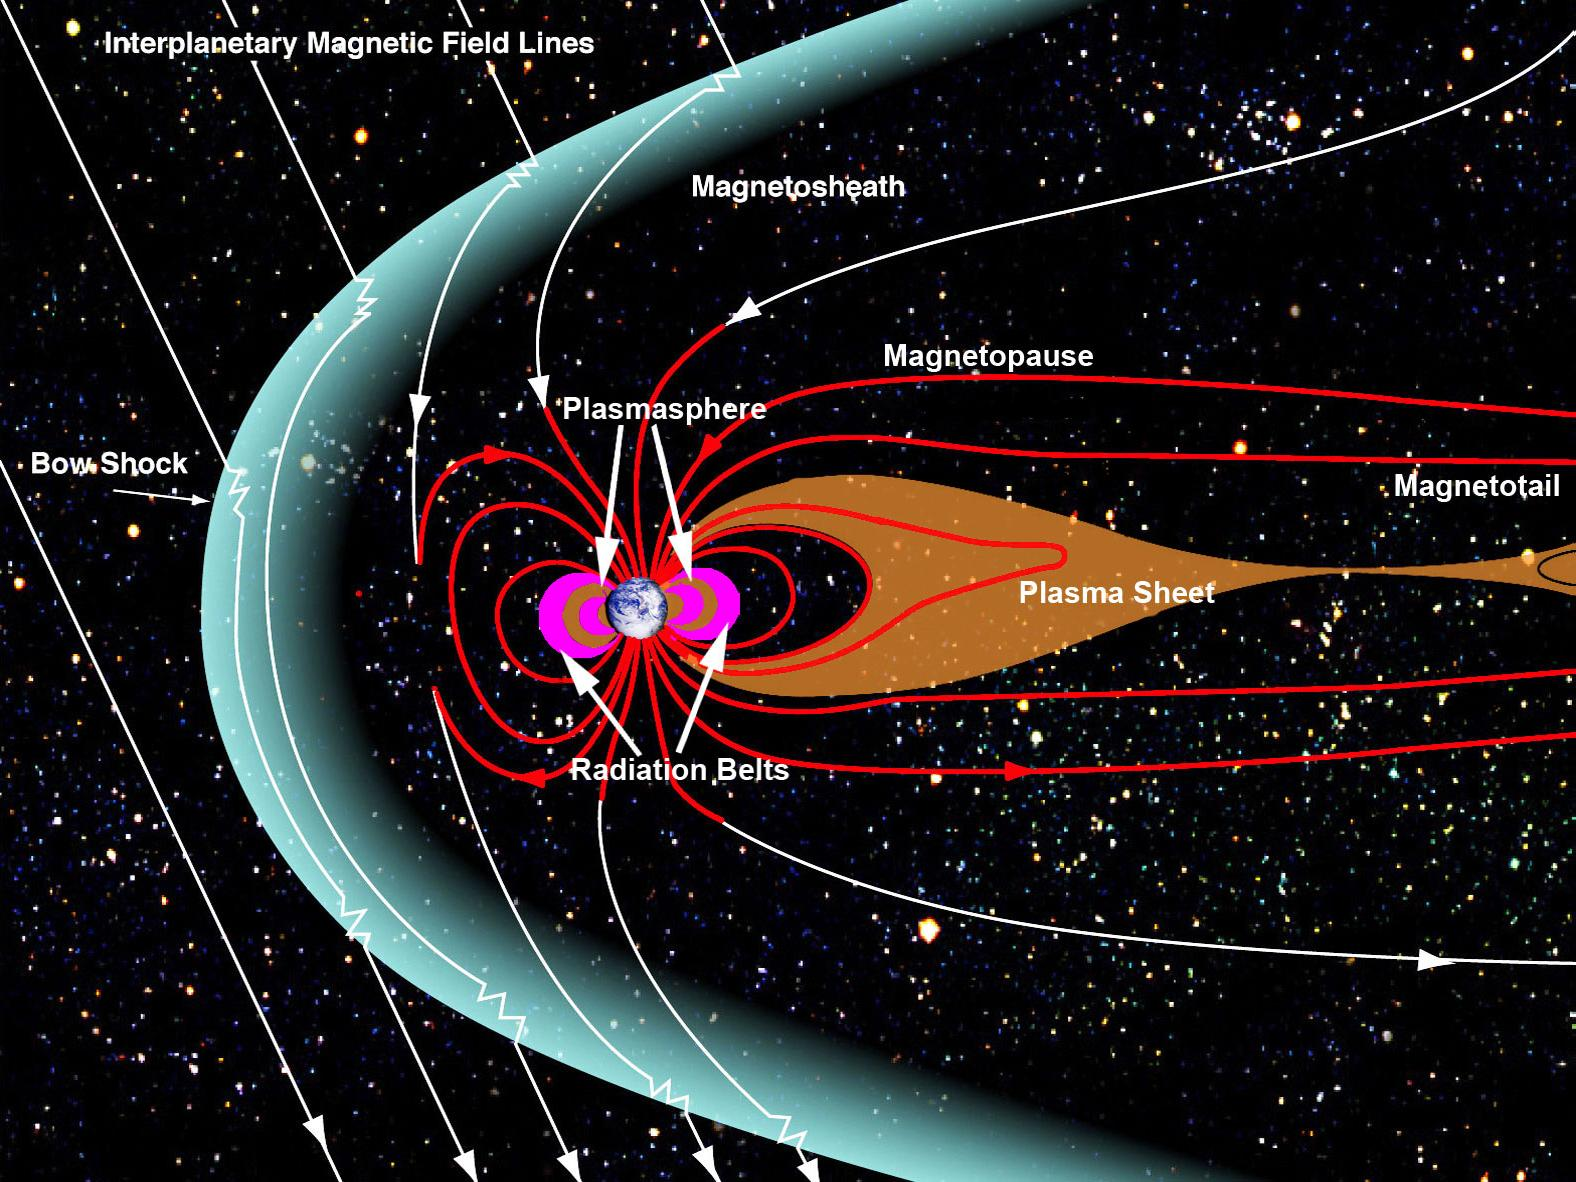
\includegraphics[width=32pc]{magne.jpg}
	\caption{Magnetosphere of the earth. Source: Aaron Kaase,NASA Goddard}
	\label{fig:magnetosphere}
\end{figure}


\section{Emissions in TI system}
Most of the energetic particles carried by the solar wind flow around this distorted magnetic field, except around the magnetic poles. Around the magnetic poles, the more perpendicular orientation of the Earth’s magnetic field allows more solar particles to enter the upper atmosphere of the Earth, either directly through the magnetic cusp (Fig. 1) or due to magnetic reconnection. In addition, there is a reservoir of trapped high energy charged particles around the Earth in regions known as the radiation belts (Fig. 1). These radiation-belt particles can diffuse or get accelerated into the upper atmosphere and interact with the upper atmosphere. Most of the entry of the energetic particles occurs at high latitudes; however, during solar storms (characterized by a sudden increase in speed and density of solar wind particles) particle precipitation can occur even at low and middle latitudes, but this depends on the strength of the storm and the orientation of IMF [3]. 
\begin{itemize}
  \item Photoionization due to high energy solar radiation plus collisional ionization by energetic particles of the upper atmospheric constituents creates a weakly ionized region known as the ionosphere (about 80-1000 km). The interaction of the electrons, called the photoelectrons or secondary electrons, depending on the process, with the neutral and ionized chemical species via collision and/or chemical processes gives rise to upper atmospheric optical emission. In general, we can categorize the optical phenomena in the upper atmosphere into two mechanisms: 

	\item  Collisional excitation due to impact of energetic charged particles generally gives rise to the aurora. These energetic particles can collisionally ionize various atomic and molecular species creating secondary electrons with different kinetic energies. These secondary electrons then change the states of the atmospheric constituents by collision and produce optical emission: line emission in the case of atoms (or atomic ions) and band emission in the case of molecules (or molecular ions). 
\end{itemize}

Photoionization, photoelectron excitation, photodissociation and other processes driven by solar radiation generally gives rise to the airglow. During the day, the solar radiation ionizes the atmospheric constituents in the upper atmosphere creating photoelectrons and dissociates molecules creating chemical species in various excited states. The photoelectrons generated by photoionization also collisionally excite chemical species into different states. During the night, the residual electrons can generate optical emission by recombination with ions. In addition, various chemical reactions in the upper atmosphere can also produce atomic (and molecular) emission. 
% put a table of main types of photochemical reactions
The six emission features that the HiT\&MIS instrument can observe are prominent emission features in the Earth’s upper atmosphere. Their main excitation processes are described in Table 1. 
%put tables of emission that hitmis can observe

\section{Energy and Auroral Emission}
The peak altitude of the electron density profile moves up or down depending on the energy of the precipitating primary electrons [3] because they are stopped at different heights based on their energy [8]. That is, the primary electrons are stopped at a lower altitude if the energy is high and thus the ionization peak moves to a lower altitude. At higher altitudes, the O (atomic oxygen) density is much higher and hence we have more O emissions due to low energy particle precipitation (Fig. 2). The $\rm N_2^+$ 427.8 nm emission can only occur at a much lower altitude as it is produced due to impact ionization and excitation of $\rm N_2$ (relative abundance higher at lower altitudes) followed by a prompt emission [5]. Even for the emission features produced by the same atom (or molecule) the exact mechanism producing the emission and the lifetimes (Table 1) determines the peak altitude where the emission takes place. So, the relative emission brightness of the four selected emissions will change differently (Fig. 2) as a function of the energy and the energy flux of the precipitating particles [9] and this information can be used to derive the energetics of the precipitating electrons. Rees and Luckey 1974 [9] use the brightness ratio of the OI 630.0 nm and OI 557.7 nm emission features and absolute brightness of the $\rm N_2^+$ 427.8 nm emission feature to estimate energy, energy flux and energy deposition rate. This proposed study will utilize four spectral features (mentioned above) observed with HiT\&MIS to derive the energy and energy flux of the precipitating electrons during auroral events. 



\section{Research Focus}
The focus of this thesis will be:
\begin{enumerate}
\item[(a)] the quantitative derivation of energy input into the Earth’s upper atmosphere during geomagnetically active times based on simultaneous multispectral measurements, and 
\item[(b)] measurement of airglow to study wave characteristics caused of Atmospheric Gravity Waves (AGWs).
 \end{enumerate} 
% \section{Problem Statement}
% How well can multi spectral measurements be used to quantitatively confine the energy inputted into the atmosphere during geomagnetically active times.

% \section{Approach}


% \section{Hypothesis and Contributions}


\import{./}{chapter1.tex}
\import{./}{chapter2.tex}
\import{./}{chapter4.tex}
\import{./}{chapter5.tex}
\import{./}{chapter6.tex}
% \documentclass[crop=false,class=mitthesis,oneside,font=12pt]{standalone}
%----------------------------Preamble-------------------------------%
\usepackage{amsmath}
%\newcommand{\angstrom}{\textup{\AA}}
\usepackage{microtype}
\usepackage{graphicx}
\graphicspath{{./images/}}
%\usepackage{multirow}
\usepackage{rotating}
\usepackage{natbib}
\usepackage{url}
\usepackage{booktabs}
\usepackage{makecell}
\usepackage{graphicx, float}            % Graphics/Images.
\usepackage{pgfplots, tikz}             % Drawing/graphing tools.
\usetikzlibrary{
    calc,                   % Calculating right angles and more.
    angles,                 % Drawing angles within triangles.
    arrows.meta,            % Latex and Stealth arrows.
    quotes,                 % Adding labels to angles.
    positioning,            % Relative positioning of nodes.
    decorations.markings,   % Adding arrows in the middle of a line.
    patterns,
    arrows,
    shapes,
    shapes.geometric,
    cd,
    hobby,
    babel
}                                       % Libraries for tikz.
\pgfplotsset{compat=1.9}                % Version of pgfplots.
\usepackage[]{pdfpages}
% for line numbers comment the next two lines before final submission
\usepackage{lineno}
\linenumbers*[1]
% use fancyhdr, to enable page style stuff (below)
\usepackage{fancyhdr}
\setlength{\headheight}{15.2pt}
\renewcommand{\headrulewidth}{0pt}

\pagestyle{plain}
\usepackage{import}                     % Import external files.
\usepackage[subpreambles=false]{standalone}      % Complileable sub files.
\begin{document}
\chapter{Measurement techniques}
In this chapter, first, the historical background on the remote sensing and in-situ measurements of the IT system, with focus on optical remote sensing is given. Then, the details of the HiT\&MIS and spectral data collection process is described. After that, the reduction and analysis of the raw data is discussed. Finally, simple descriptions on other instruments and measurements used in this thesis is provided.
\label{chap:background}
\section{Overview}
%Balfour Stewart suggested existence of conducting layer of charged "air" in the upper atmosphere from small perturbations seen in magnetic measurements.
Measurements of the IT system is generally done using various plasma, neutral and optical measurement techniques. These include different radio measurement techniques, in-situ mass spectrometers, all-sky imagers, etc. Among radio techniques, the time profile of reflected or back-scattered radio waves are used to probe ionospheric parameters. Incoherent Scatter Radar (ISR) method works by sending high power radio wave at a fixed frequency into the ionosphere. The back-scattered profiles of the radio waves along with exact theoretical modeling is then used to infer density, velocity, temperature and spatial morphology of ionospheric plasma. Similarly, free electrons act as mirrors to radio waves below a critical frequency known as the plasma frequency, and so can act as a probe of ionospheric plasma using ionospheric sounding (ionosondes). Ionosondes operate by sending radio waves in a sweep of frequencies and then measuring the time profile of the reflected waves to infer electron densities. In addition to these radio techniques, GPS based radio transmitters can be used to probe the ionosphere by measuring the change in power and phase (brought about by the ionosphere) received at detectors on the ground to derive the line-of-sight integrated columnar electron density, also known as the Total Electron Content (TEC). 

Since the ionosondes requires small, portable radio wave generators and detectors, a network of ionosondes can be created (for example see \citet{giro}). While ISRs require large radio antennas, they can provide local spatial variations and be used to probe more plasma parameters (like temperatures and velocity) which ionospheric sounding can't probe. Similar to ionosonde, measurements form multiple network of GPS satellites allows for maps of TEC over large areas to be constructed, providing global morphology. 

Other measurement of the IT system include various in-situ charge particle detectors, mass spectrometers, etc., that can make direct measurements of plasma and neutral densities. Furthermore, optical measurements from ground and space can also be used to study the IT system if the processes involved in the observed emission is known. 

\subsection{Optical Remote Sensing}

Optical remote sensing of the IT system is a passive remote sensing technique as the airglow/auroral emissions act as proxies to IT processes. Early satellite based measurements of the upper atmosphere provided a wealth of information on prominent emission mechanisms and morphologies. For example, the limb scanning methods provided information on the altitude profiles of different airglow/auroral emissions and helped to better understand the processes leading to these emission. Satellite based optical measurements also provide large scale emission brightness morphologies at different latitude and longitudes, as well as, day/night variability. Red-line measurements from the Visible Airglow Experiment (VAE) which was on board the Atmospheric Explorer-C satellite, in conjunction with modeling was used to investigate the detailed photo-chemistry that give rise to the emission \citep{hays1978}. Using the green-line measurement from the same instrument, \cite{frederick1976} discussed processes that leading to the emission. In addition, \citet{orsini1977determination} discuss the photo-chemistry of the N$_2^+$ 427.8 nm vibrational band emission and  showed the height of its peak emission varies with season and magnetic activity. Further, sounding rocket experiments with multiple instruments can provide vertical profiles of auroral and airglow emission as well as in-situ plasma and/or neutral measurements near simultaneously. Such an approach is not only useful in getting the altitude profiles of emissions, but also to identify and constrain contribution of different sources that give rise to a particular emission.

While satellite-based optical measurements provide excellent spatial coverage, they lack temporal coverage at a given location. The ground-based instruments, on the other hand, lack the spatial coverage but can be used to observe temporal evolution of emission intensities. Ground-based photometric and/or spectrometric emission measurement also allow us to study IT system at different altitudes provided the emission sources are understood. Some of the information that can be inferred include the following:
\begin{itemize}
\item the column density of the emitting species has direct relationship with the emission intensity. So, if the optical instrument is photo-metrically calibrated the column density of emitting species can be retrieved.
\item Assuming thermal equilibrium between the surrounding and the emitting species, the line profile of an emission can be used to estimate the Doppler temperature and line of sight winds provided the line profile has enough resolution.
\item Provided the rotational structure of molecular emission is sensitive to the ambient gas temperature it can be used to estimate ambient gas temperature. Several band emissions that occur within the IT system, including the N$_2^+$ 427.8 nm, are sensitive to the ambient gas temperature.
\item The spatial and temporal changes in airgloe brightnesses can be used to study atmospheric dynamics caused by events like AGWs.
\item Simultaneous multi-spectral emission brightness measurements, can be used to study vertical propagation of atmospheric dynamics, such as during AGW events.
%In addition to the optical remote sensing 

%Various optical instruments have flown in rockets to investigate airglow and auroral emissions at different wavelength ranges
\end{itemize}

\section{HiT\&MIS}

The spectral data used in this thesis was collected using the HiT\&MIS instrument, which is a high-resolution ($\approx$ 0.02 nm at 630.0 nm) spectrograph, that can work on a round the clock basis \citep{hitmis}. HiT\&MIS follows a list of similar imagers that use a combination of slits, interference filters with the Echelle grating to select and image emission features of interest. These instruments include High Throughput Imaging Echelle Spectrograph (HiTIES, \cite{hities}), High-Resolution Imaging Spectrograph using Echelle grating (HIRISE, \cite{hirise}), Multi-wavelength Imaging Spectrograph using Echelle grating (MISE, \cite{mise}), Continuous High-resolution Instrument for Multiwavelength Echelle Spectroscopy (CHIMES, \cite{chimes}), etc. Each instrument was designed to image specific emissions at specific settings. For example, HiTIES was designed for night-time/twilight-time measurements, while CHIMES was designed for daytime measurements. These measurement constraints arise because requirements for daytime and night-time/twilight-time imaging are different. During the daytime, the solar background is orders of magnitude higher than the airglow/auroral emission signal, and thus high resolution is required to match with a solar reference spectrum so that the solar contribution can be subtract out. To obtain this, maximum dispersion of collected light is necessary which is achieved by using narrower slits as the throughput is not an issue during the day. During nighttime, the slit needs to be wide enough to have a enough throughput at reasonable temporal resolution. Thus, for round-the-clock measurement, the instrument needs to be designed to match both high-throughput and high-resolution requirements and be portable (Figure \ref{fig:hitmis_tripod}). This is where HiT\&MIS comes into consideration.

\begin{figure}[H]
	\centering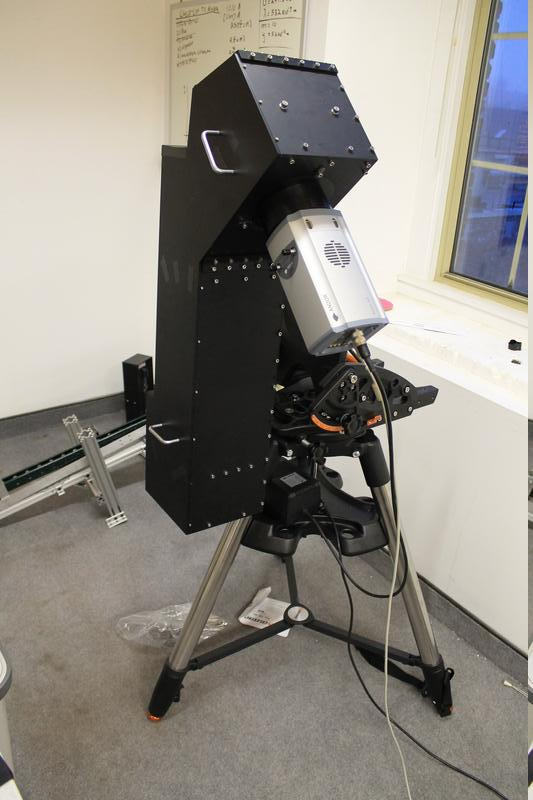
\includegraphics[width=25pc]{Hitmis_tripod_mount.JPG}
	\caption{HiT\&MIS mounted on a tripod. The portable design makes it versatile for campaign at different locations.}
	\label{fig:hitmis_tripod}
\end{figure}

The theoretical design of HiT\&MIS is schematically shown in Figure \ref{fig:hitmis}. It has a field of view of approximately 0.1$^\circ$ $\times$ 50$^\circ$ and a dispersion of about 0.02 nm/px in its current iteration.  Light enters through the four slits (numbered 1-4 in Figure \ref{fig:hitmis}), each of which is fitted with a narrow band filter (transmission properties listed in Figure \ref{fig:hitmis_tr}). There is also a mosaic of filter that is placed at the image plane. The light that has passed through the slits and the four entrance filters passes through a collimating lens (collimator/camera in Figure \ref{fig:hitmis}) and gets dispersed by the echelle grating in a near Littrow configuration. The diffracted light goes back into the same collimating lens that now acts as an imaging lens into a mosaic of interference filters (image plane filters in Figure \ref{fig:hitmis}). This combination of filters at the slits and the mosaic filters determines what spectral information is imaged. The image is then reflected through a folding mirror and refocused via a camera lens onto the CCD detector \citep{hitmis}.
\begin{figure}[H]
	\centering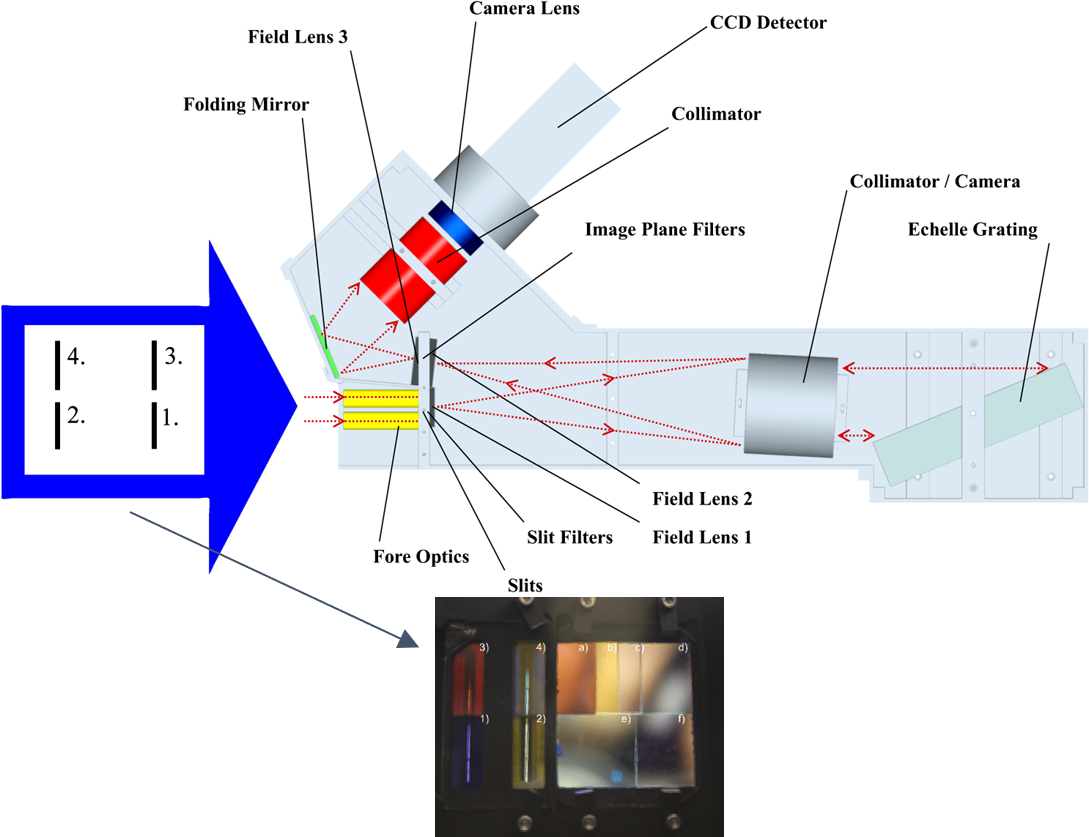
\includegraphics[width=25pc]{hitmis.png}
	\caption{Schematic diagram of the internal optics of the HiT\&MIS instrument. Adapted from \cite{hitmis}.}
	\label{fig:hitmis}
\end{figure}
%%%
\begin{figure}[H]
	\centering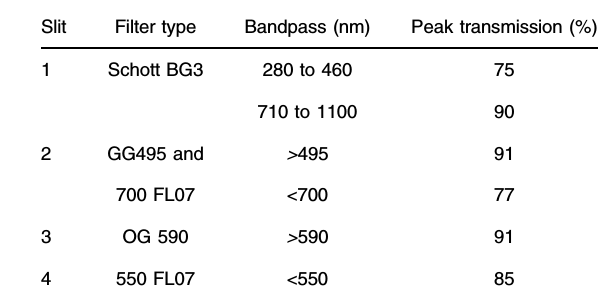
\includegraphics[width=25pc]{hitmis_tr.png}
	\caption{The transmission properties of the interference filters used in HiT\&MIS. Source: \cite{hitmis}.}
	\label{fig:hitmis_tr}
\end{figure}


HiT\&MIS has been developed to observe airglow and auroral emissions simultaneously at six selected wavelengths on a round-the-clock basis. The selected spectral features are: HI 656.3 nm, HI 486.1 nm, OI 557.7 nm, OI 630.0 nm, OI 777.4 nm and N$_2^+$ 427.8 nm. These emissions are key diagnostics to study the processes involved in airglow and aurora in detail. The six emission features that the HiT\&MIS instrument can observe are prominent emission features in the Earth’s upper atmosphere. The main excitation processes for the four emission features imaged by HiT\&MIS and used in this thesis are described in Table \ref{tbl:hm_emi}. 
%put tables of emission that hitmis can observe

%%%%%
%%%%
\section{HiT\&MIS Data Analysis}
%For this study, we used three spectral features observed by HiT\&MIS: blue line, green line and red line. 
\subsection{Characterization of CCD }
The spectral images were recorded using an Charged Coupled Device (CCD) camera cooled to -59$^\circ$ C. CCD cameras are semiconductor devices where photons that hit the CCD detector eject electron via the photo-electric effect and are excited to the conduction band where they can then be counted. To characterize the CCD, the bias frame and the dark frame were obtained by taking images with varying exposure times while the shutter was closed. The bias frame is a fixed pattern noise present in CCD images as a result of random quantum mechanical thermal fluctuations. Data counts (in Arbitrary Data Unit, ADU) on each pixel were then fitted to a linear equation to estimate the bias, B (in ADU)  and the dark frames, D (data units/s). The histograms for the bias and the dark frames are shown in Figure \ref{fig:biasdark}.  

\begin{figure}[H]
	\centering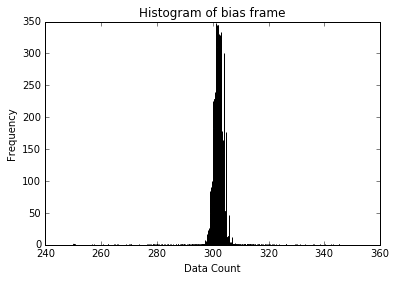
\includegraphics[width=30pc]{bias.png}
    \centering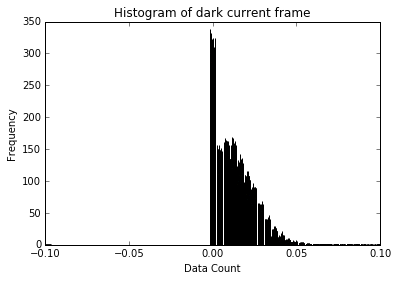
\includegraphics[width=30pc]{dark.png}
	\caption{Top: Histogram of the master bias, with a mean value of $\sim$ 300 ADU/pixel.  Bottom: Histogram of the master dark current, with mean value of 0.019 ADU px$^{-1}$ s$^{-1}$.}
	\label{fig:biasdark}
\end{figure}

\subsection{Emission line-center calibration}
\begin{figure}[H]
	\centering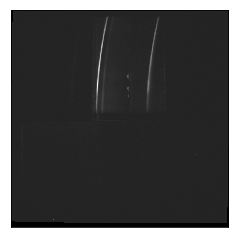
\includegraphics[width=20pc]{night_raw.png}
    \centering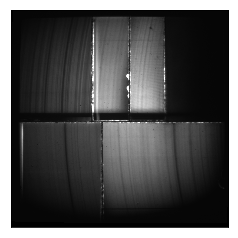
\includegraphics[width=20pc]{day_raw.png}
	\caption{Top: Sample night-time raw image from HiT\&MIS at 22:30 PM LT on June 22, 2015 with 60 s exposure. Bottom: Sample daytime raw image with 0.1 s exposure time at 17:30 PM LT on ths same day. Notice couple of spectral emission features are visible at night while absorbtion features are visible during the day.}
	\label{fig:raw_1}
\end{figure}
%
Figure \ref{fig:raw_1} shows an example of raw images collected by HiT\&MIS during day and night. While designing HiT\&MIS a ray trace simulation that was initially used to determine the different filters used instruments \citep{hitmis}. A set of filters were chosen to only let in lights around wavelength of interest and the emission features dispersed by the echelle was simulated (see Figure \ref{fig:hit_if}, top). Based on this ray trace result, mosaic of filters were chosen to select only the wavelength's of interest and the a ray trace was generated again using both entrance and the imaging mosaid filters (Figure \ref{fig:hit_if}, bottom). This final ray-trace can also be utilized to find the emission line center location on the CCD. During night, with enough cadence ($\sim$~60 s+) the red and the green lines are clearly visible on the detector (Figure \ref{fig:raw_1}, top). Similarly, during the day, the H$_\alpha$ and H$_\beta$ emissions show up as absorption features in the raw image (Figure \ref{fig:raw_1}, bottom). Thus, the ray trace results can be over-laid over the four emission feature location in the to validate the ray-trace simulation estimates as well as to to find emission line center locations. 
\begin{figure}[H]
	\centering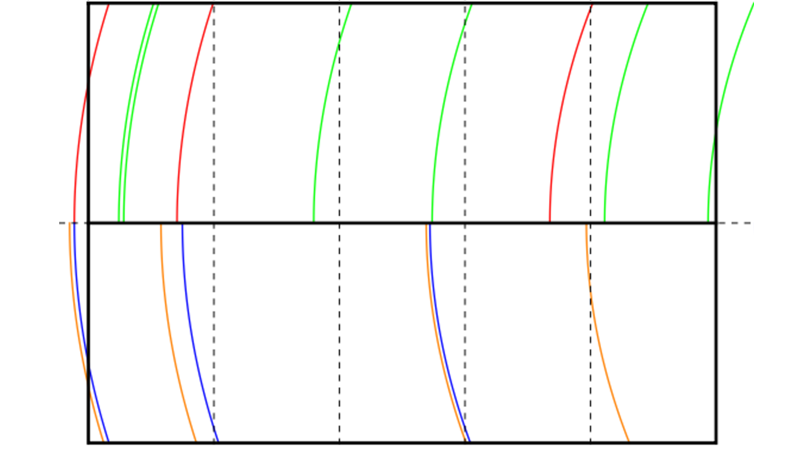
\includegraphics[width=30pc]{hit_i.png}
    \centering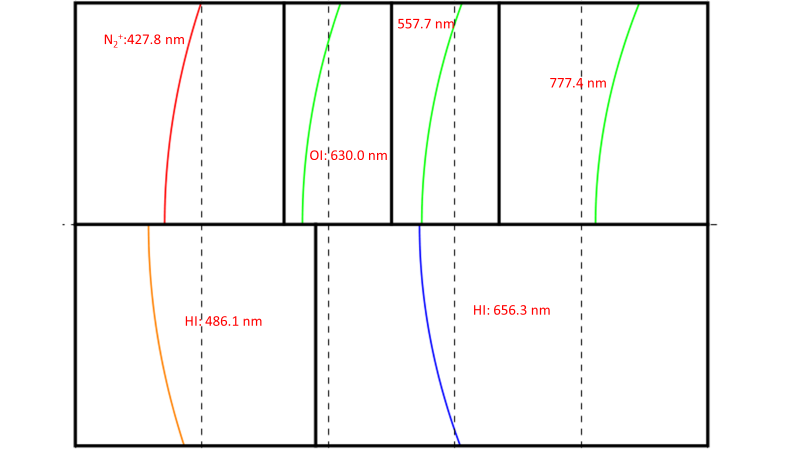
\includegraphics[width=30pc]{hit_f.png}
	\caption{Top: Ray trace modeling of emission lines from HiT\&MIS with only the entrance slits and filters. Bottom: Ray trace modeling of emission lines of interest from HiT\&MIS with the entrance slits and filters plus the image plane mosaic of filters. Notice that the overlapping lines disappear with the inclusion of mosaic of filters. Plot generated by Kuravi Hewawassam, UML}
	\label{fig:hit_if}
\end{figure}

The details of the the ray-trace simulation, similar to (but not the same) that used in \cite{hitmis} are now provided. To start, the following assumption were made to simplify the problem:
\begin{itemize}
\item all the filters were assumed to let in lights within $\pm$ 20 nm from central wavelength.
\item No estimates of the intensity was included, the light either came through or they didn't (binary scheme).
\item Only the wavelength of interest were let into the entrance filters.
\item The line from the center of the all the slits to the center of the Echelle are perpendicular.
\item The distance between the grating and the entrance slits and imaging mosaic filters are equal
\end{itemize}
%%
\begin{figure}[H]
	\centering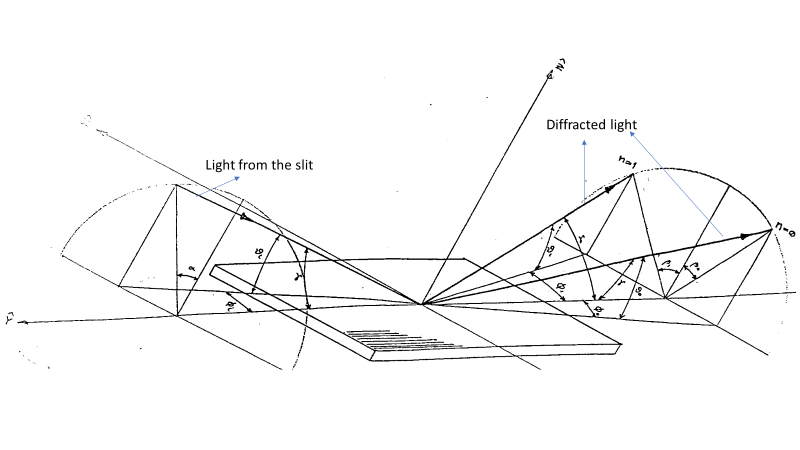
\includegraphics[width=35pc]{grating_stp.png}
	\caption{Geometry of spectral dispersion from to a grating. }
	\label{fig:grating}
\end{figure}

The light that entered through the entrance filters, now encountered the Echelle grating that disperses the light with the following grating equation:
%%
\begin{equation*}
\large
{n~\lambda~=d~sin\gamma~(sin\alpha + sin\beta_n)}
\end{equation*}
%%
\begin{equation}
\large
\implies~~\beta_n~=sin^{-1}\Big(\frac{n~\lambda~}{d~sin\gamma~}~-sin\alpha\Big).
\end{equation}
Here, d is the groove density of the grating, $\beta_n$ is the dispersion angle of the n$^{th}$ order at a particular ray entering through the slit at an angle $\gamma$ with respect to y-axis (see Figure \ref{fig:grating}). By measuring possible range of angles between the grating and the slit, the emissions at the imaging plane were simulated by taking following steps:
\begin{itemize}
\item Step1: Simulate all the emission lines passing through the slits, entrance filters and the grating (Figure \ref{fig:hit_if}, top). 
\item Step 2: Simulate the emission line that pass through the entrance slits that get dispersed by grating and select the mosaic of filters at the imaging plane that would only allow emissions of interest to pass through (Figure \ref{fig:hit_if}, bottom).
\end{itemize}
Once the ray-trace estimation location were made to match what was seen in the raw image (Figure \ref{fig:raw_line}), the region around the emission of interest are extracted for further analysis (Figure \ref{fig:cut_hm}). 
\begin{figure}[H]
	\centering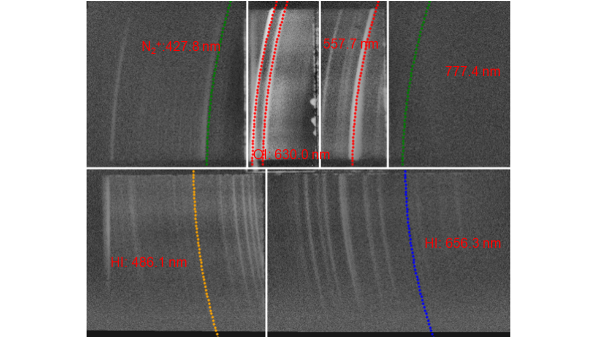
\includegraphics[width=32pc]{night_hm.png}
    \centering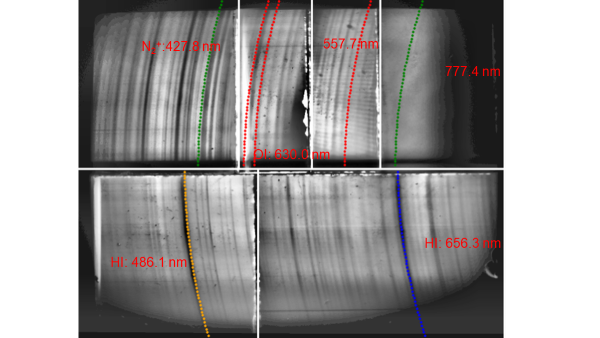
\includegraphics[width=32pc]{day_hm.png}
	\caption{Top: Sample night-time raw image from HiT\&MIS at 22:30 PM LT on June 22, 2015 with 60 s exposure. Overlaid lines are the ray trace estimate of the line center locations of the emission features shown in Figure . Bottom: Sample day-time raw image with 0.1s exposure. Notice that some of the emission feature at night-time image and absorption features and align with the ray-trace estimates.}
	\label{fig:raw_line}
\end{figure}

\begin{figure}[H]
	\centering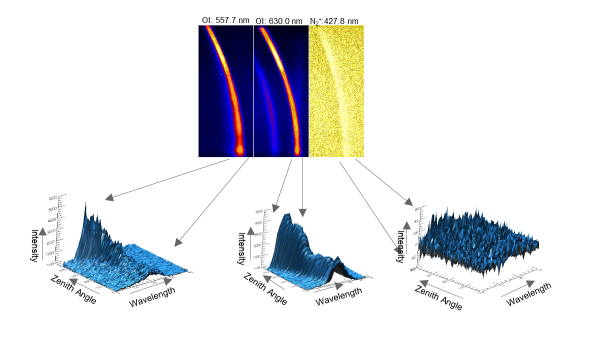
\includegraphics[width=35pc]{cut_hm.png}
	\caption{Top: Sample night-time raw image from HiT\&MIS at 22:30 PM LT on June 22, 2015 with 60 s exposure for the red line, green line and the N$2^+$ 427.8 nm. Bottom: Cut of background spectra extracted from Top.}
	\label{fig:cut_hm}
\end{figure}

\subsection{Photo-metric calibration}
HiT\&MIS creates spectral images of emissions as a function of wavelength and zenith angle (Figure \ref{fig:cut_hm}). For each spectral feature, the emission region over a narrow range of wavelength ($\approx$ $\pm$0.3 nm from the line center) was extracted from the image as mentioned in the last section. Then, the curvature in the measured spectrum as a function of zenith angle due to the slit geometry was corrected by transforming the cut-out spectral image such that the pixels with emission peaks are moved to the center. Finally, the baseline was estimated by averaging values on both side of the spectral feature and subtracted from the data, to obtain the signal, S. This gives the spectral signal (S), the background (B) and the readout noise (RN, standard deviation of the bias frame). The background subtracted spectra (un-calibrated) can now be represented as: $S \pm \sqrt{(S+B) + RN^2}$.  The analysis presented here applies only for night time data analysis. Possible daytime spectral imaging procedure for spectral imagers like HiT\&MIS is provided in Chapter 5.


\begin{figure}[H]
	\centering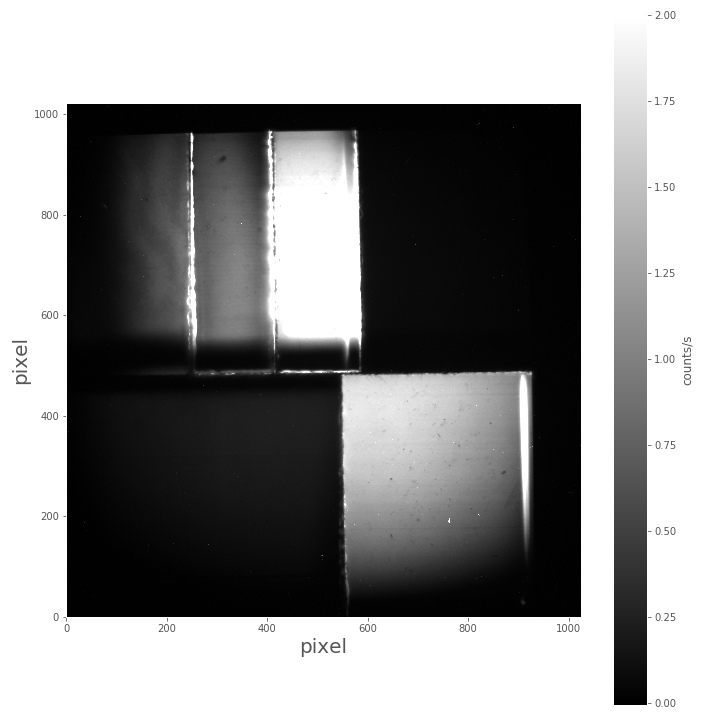
\includegraphics[width=30pc]{sen.png}
	\caption{Noise reduced master sensitivity image obtained by illuminating a calibrated lamp on to HiT\&MIS. As the output of the lamp as a function of the wavelength is known, this image was used to convert background subtracted data counts to photon counting units. }
	\label{fig:sen}
\end{figure}

A C-14 activated light source was used to calibrate the signal photo-metrically. This was done by illuminating HiT\&MIS with the calibration lamp for different increasing exposure times. These images were dark noise subtracted and averaged to get an the sensitivity of the instrument (in ADU per seconds) at each pixel (Figure \ref{fig:sen}). The output of the lamp is known and this was used to calibrate image data counts to physical units (in Raleigh $\rm {\AA}^{-1}$, see Figure \ref{fig:calib}, top). The calibrated spectra can then be averaged over different look direction bins (see Figure \ref{fig:calib}, bottom) to obtain a representative spectrum. Integrating the spectrum along the wavelength axis gives the line of sight brightness at different look directions. 
\begin{figure}[H]
	\centering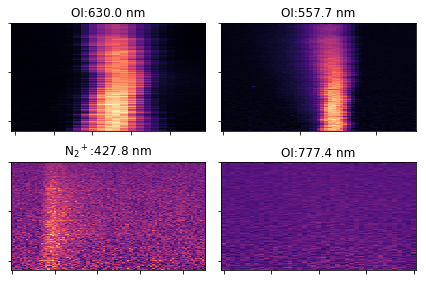
\includegraphics[width=30pc]{feature_img.png}
    \centering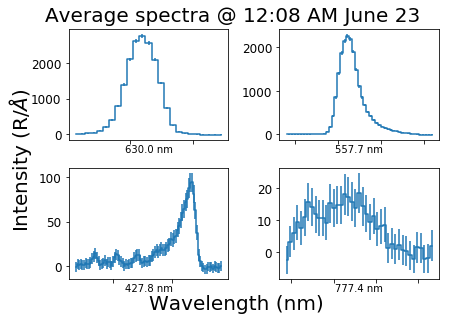
\includegraphics[width=30pc]{feature_spectra.png}
	\caption{Top: Curvature (due to slit geometry) straitened, noise reduced and photometrically calibrated spectra in red line, green line, blue line and OI 777.4 nm. Bottom: Same as top but averaged over look directions.}
	\label{fig:calib}
\end{figure}

\section{Other Measurement Techniques}
In addition to the optical remote sensing techniques, other techniques directly or indirectly used in this thesis are described in brief below. 

\subsection{Incoherent Scatter Radar (ISR)}
While ISR derived results are not used directly in this thesis, various other work cited in this thesis use ISR derived parameters extensively and thus a simplified picture of ISR is provided. Since the early 1960's, the Incoherent Scatter Radar has been the most used techniques to probe the ionosphere. This technique utilizes the incoherent scattering of the radio waves by ions and electrons in the ionosphere which occurs when the wavelength of the probing radio wave is smaller than the Debye length \citep{dougherty1963theory}. Above the Debye length (see Chapter 1) the charge particles are affected by each other such that the collective properties becomes coherent, both spatially and temporally. In general, the ISR measurements are not completely incoherent or coherent, however if the profiles of the incoherent back scatter are known they can be compared with theoretical models to obtain ionospheric parameters. 
%%%%
\begin{figure}[H]
	\centering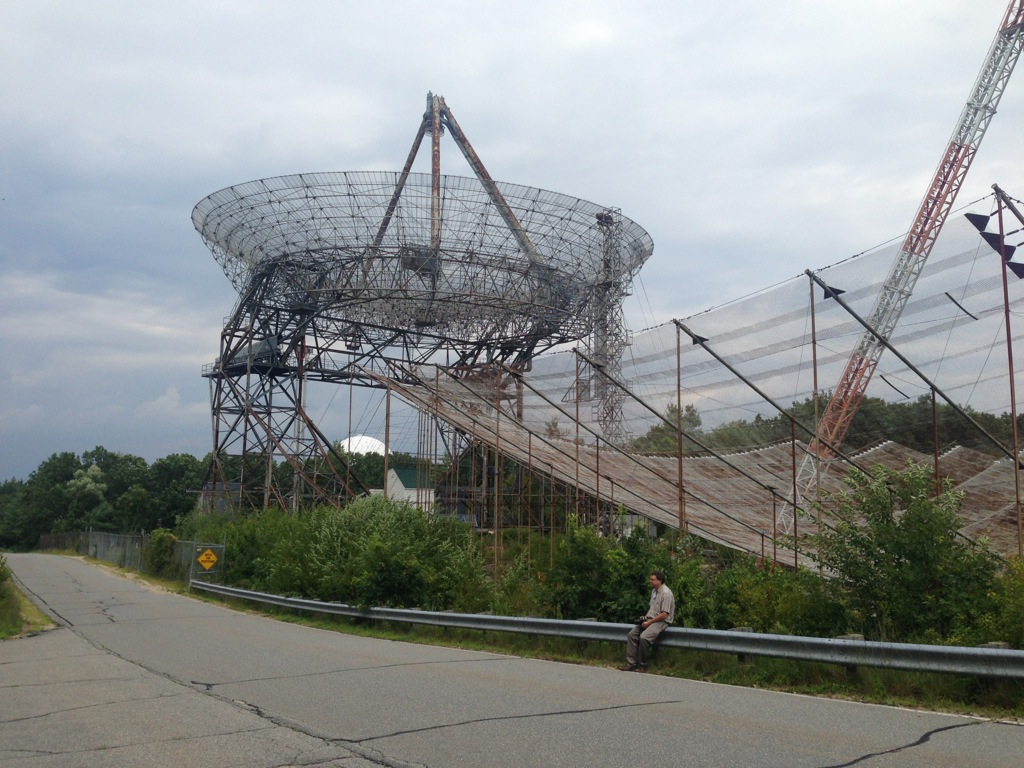
\includegraphics[width=30pc]{isr.jpg}
	\caption{ISR at MIT Haystack. Source: \url{http://blog.eiscat3d.org/2013/08/millstone-hill-incoherent-scatter-radar.html}}
	\label{fig:isr_a}
\end{figure}

The ISR technique works by sending high power radio waves at a fixed frequency, using a giant transmitter and antenna setup (see Figure \ref{fig:isr_a}). These radio-waves are then back-scattered by the electrons and ions incoherently which can be used to infer the their bulk properties. Since the ions are orders of magnitude heavier than the electrons, in frequency domain, the radio-waves back-scattered by the electrons and ions have completely different profiles (Figure \ref{fig:isr}), and hence can be used to probe both. In a simplified picture, the shift in frequency, the doppler width, and the area of the back-scattered profiles then are related to the line of sight velocity, the temperature and the plasma density, respectively. The radio-pulse sent to probe the ionosphere for ISR measurements, can be coded depending on the phenomenon to be studied and the altitude of focus.
\begin{figure}[H]
	\centering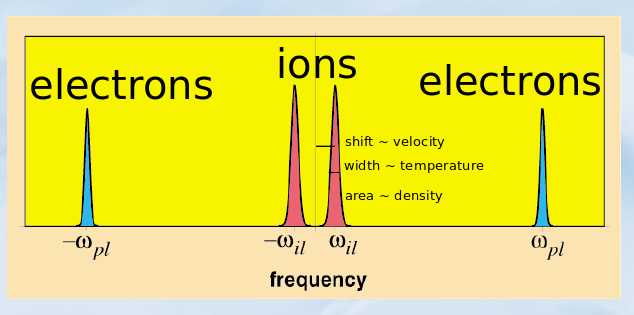
\includegraphics[width=30pc]{isr.png}
	\caption{ISR back scatter profile, and what different part of the profile signify. Adapted from \cite{anja}.}
	\label{fig:isr}
\end{figure}

\subsection{GPS-based Total Electron Content (TEC)}
Global Positioning System (GPS) uses multiple earth orbiting satellites ($\sim$ 32+) to mathematically triangulate a position on Earth. While GPS satellites are not geo-synchronous, if at least four satellites are visible at a given time, a receiver can accurately determine its location and velocity with the help an atomic clock (accuracy of 1 billionth of a second). As GPS technology uses radio signals to operate, the ionospheric plasma modulate the signal via radio waves plasma interaction. This modulation in both phase and amplitude of the signal is a proxy to the total electron content (TEC) the signal encounters along its path. With multiple receivers and GPS satellites, a map of the TEC can be made to study the effect of different phenomenon in the IT system. In this thesis, the Differential TEC( DTEC), which is the dynamic part of the TEC is used to study plasma waves in the IT system.
\begin{figure}[H]
	\centering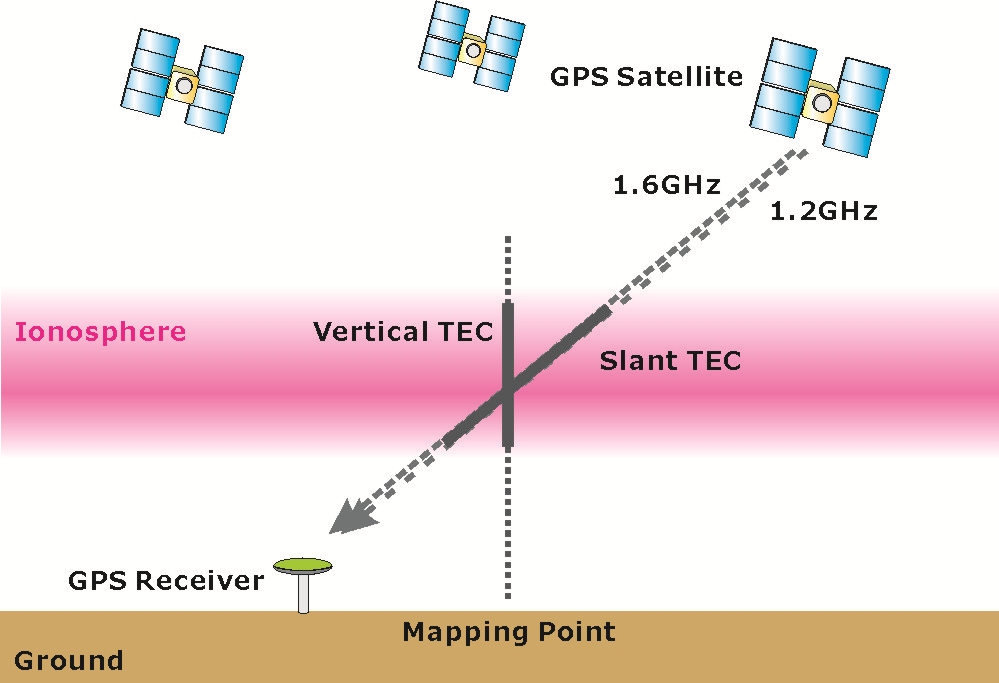
\includegraphics[width=30pc]{6-0.png}
	\caption{Schematic of GPS based TEC measurement. Source: \cite{tsugawa}.}
	\label{fig:gps}
\end{figure}

\subsection{Vertical Ionospheric Sounders (Ionosondes)}
Ionospheric sounding is another radio measurement technique to probe ionospheric plasma. It uses reflection of radio-waves above a critical frequency from the ionospheric plasma. Since the ionosphere is stratified into different plasma density peaks (Chapman layers), by probing in a range of radio frequencies, a vertical profile of the plasma density inferred. Thus, ionosonde broadcast radio waves at different frequencies which are then reflected only at certain frequencies from a particular ionospheric height which is then detected at ground (see Figure \ref{fig:digi_im} for the ionosonde setup). However, since the receiving times are different depending the altitude of reflection, an ionogram (like \ref{fig:digi_is}) is generated that can be converted into electron density profile.
\begin{figure}[H]
	\centering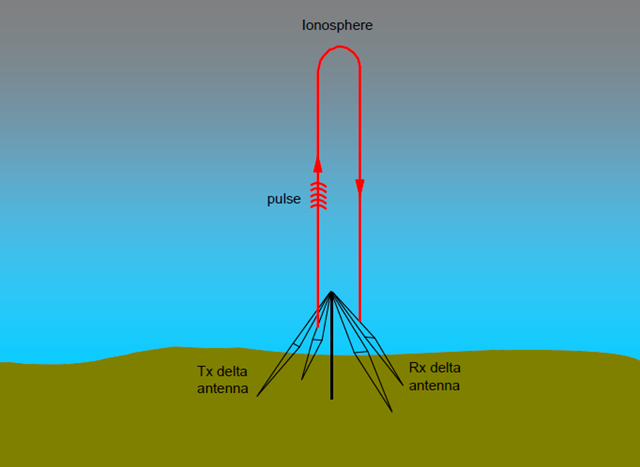
\includegraphics[width=30pc]{ionosonde.png}
	\caption{Schematic of a ionosonde system. Source: \cite{heather}.}
	\label{fig:digi_im}
\end{figure}

The index of refraction, n, for a radiation with frequency, f, incident on an electron distribution with density, N$_e$,  is given by:
\begin{equation*}
n^2~=~\Big(1~-~\frac{N_{e}~e^{2}}{4~\pi^{2}~\epsilon_{0}~m_{e}~f^{2}}\Big).
\end{equation*}
By defining a critical frequency, f$_c^2$ = $\frac{N_e~e^2}{4~\pi^{2}~\epsilon_{0}~m_{e}}$ , the index of refraction can be written as:
\begin{equation}
n^2~=1~-~\Bigg(\frac{f_c}{f}\Bigg)^2.
\end{equation}

From the equation \theequation, it follows that  the index of refraction for frequencies below the critical frequency (f $<$ f$_c$) is purely imaginary; at frequencies above the critical frequency (f $>$ f$_c$) it is purely real, and zero when the frequency of incident radio wave is equal to the critical frequency (f = f$_c$). This implies that at if the incident radiation is higher than the critical frequency of the medium, it penetrates the medium, where as below this frequency it is purely reflecting. Thus, if the ionosphere, with stratified ionization peaks (during the daytime), is probed with a sweep of frequency around the critical frequency a reflection profile as a function of frequency and reflection time (ionogram) can be created as shown in Figure \ref{fig:digi_s}. The ionogram can then be used to infer the electron density (by knowing f$_c$) profile as the time of return on to the detector measuring the reflection also gives information about the height were a particular frequency of radio wave was reflected from.
\begin{figure}[H]
	\centering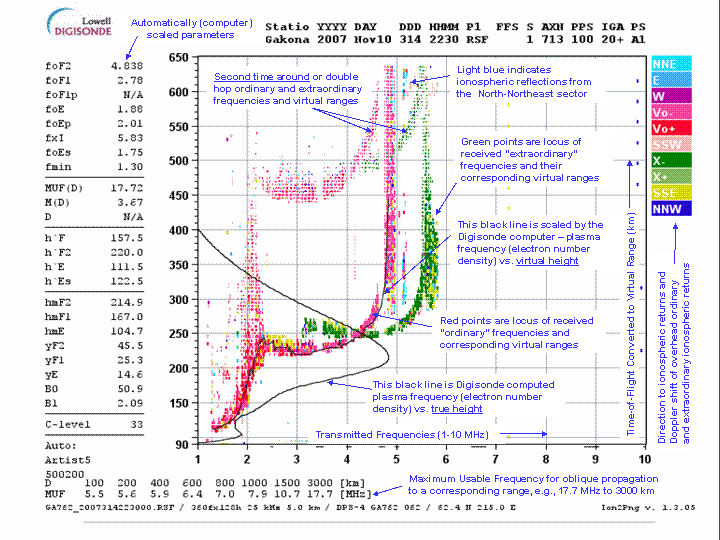
\includegraphics[width=30pc]{HAARP_ionogram.png}
	\caption{An example of a Ionogram. Source: \url{https://www.hfunderground.com/wiki/Ionosonde}}
	\label{fig:digi_s}
\end{figure}


\subsection{Magnetometers}
Magnetometers can be used to make precise measurement of the magnetic fields. While there are magnetometers that sense the magnetic field using other principles, only the fluxgate magnetometer is discussed herein. 

\begin{figure}[H]
	\centering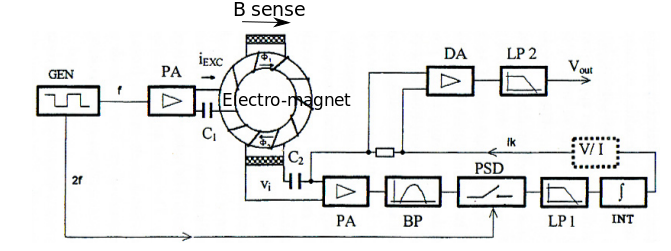
\includegraphics[width=30pc]{magnto.png}
	\caption{Schematic a single axis fluxgate magnetometer, with the sensing direction shown. Source: adapted from \cite{ripka2001magnetic}}
	\label{fig:magnemtr}
\end{figure}

Based on \citep{ripka2001magnetic}, a coil of wire with N turns and area A wrapped around a core with high relative magnetic permeability $\mu_r$; the magnetic constant $\mu_0$, a changing magnetic field B, with associated flux $\Phi$, will induce a voltage V such that,
\begin{equation*}
V~= \frac{d}{dt}\Phi~~=\frac{d}{dt}(N~A~\mu_{0}~\mu_{r}~B),
\end{equation*}using the Faraday's law. If B, A, and $\mu_r$ are functions of time, the voltage, V can be written as,
\begin{equation}
V=~N~A~\mu_{0}~\mu_{r}\frac{dB}{dt}+N~A~\mu_{0}~\mu_{r}~B\frac{dA}{dt}+N~A~\mu_{0}~B\frac{d\mu_{r}}{dt}
\end{equation}
From, equation \theequation, it is seen that modulating $\mu_r$ allows for the magnetic field B to be sensed. The discussion so far has been on a single axis magnetometer, where magnetic field component along one direction can be measured. However, changing the design of the magnetometer makes it possible to sense magnetic filed along three orthogonal axis. In this thesis, measurement of the Earth's magnetic field using AMPERE and the strength of ionospheric currents computed from these measurement is used.
\begin{figure}[H]
	\centering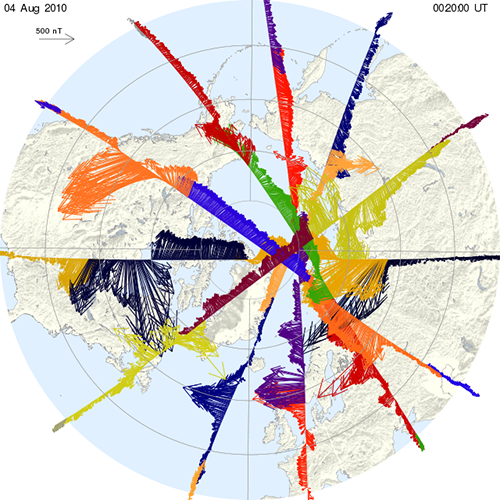
\includegraphics[width=30pc]{fac_s.png}
	\caption{Magnetic field in the polar region. The perturbations in these magnetic field can be used to infer the Field Aligned Current. Source: Johns Hopkins University Applied Physics Laboratory/AMPERE/R. J. Barnes}
	\label{fig:fac_s}
\end{figure}

\subsection{All Sky Imagers (ASIs)}
All sky imagers use narrow-band interference filters ($\sim \pm$ 20 nm from the central wavelength) and fish-eyed lens to image airglow/auroral emissions over the whole sky as seen from a particular location. This setup allows one to study the latitudinal/ longitudinal coupling of airglow/auroral emissions. Figure \ref{fig:asi_s} shows a typical all-sky imager setup. 
\begin{figure}[H]
	\centering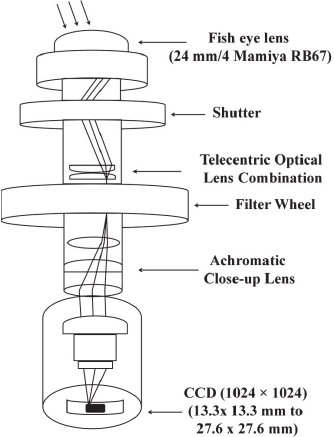
\includegraphics[width=30pc]{asi.jpg}
	\caption{Schematic example of a all-sky imager setup. Source: \cite{nade2012occurrence}}
	\label{fig:asi_s}
\end{figure}

ASI's give 2D auroral/airglow brightnesses; however, no spectral information can be obtained and thus there is a need to deal with contamination from nearby spectral features. This is in contrast with spectral imagers (like HiT\&MIS), where higher spectral resolution ($\sim$ 0.1 nm or less) allows for only the brightness feature of interest to be extracted, however only 1D airglow/auroral brightnesses (along the slit) can be observed.
\begin{figure}[H]
	\centering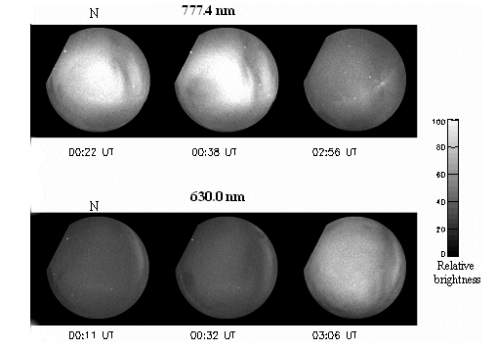
\includegraphics[width=30pc]{asi_mul.png}
	\caption{Near simultaneous raw ASI images in red line and OI: 777.4 nm at El Leoncito, Argentina on 30 May, 2003. From \cite{martinis2006imaging}  }
	\label{fig:asi_mult}
\end{figure}

Typically, ASI's use filter wheels to image multiple emissions of interest near simultaneously. Figure \ref{fig:asi_mult} shows near simultaneous raw ASI images at red line and OI: 777.4 nm line. Since the fish eye lens projects the features that are more spherical in 3D (due to the Earth's geometry) into a 2D image, the images near the edges are stretched. Thus, to project these emissions on to the map they are typically transformed based on the geographic location of the ASI and the peak height at which the emissions occur (see Figure \ref{fig:asi_urap}).

\begin{figure}[H]
	\centering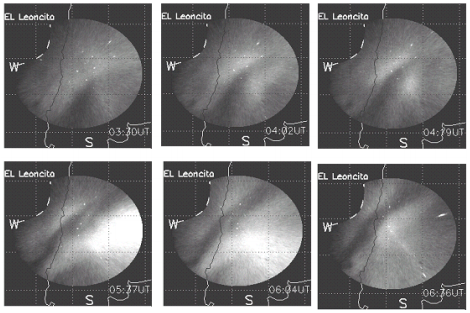
\includegraphics[width=30pc]{asi_urap.png}
	\caption{An example of all sky images in red line that has been transformed to be geographycally mapped. From \cite{martinis2006imaging} }
	\label{fig:asi_urap}
\end{figure}

\end{document}
% \include{chapter3}
% \documentclass[crop=false,class=mitthesis,oneside,font=12pt]{standalone}
%----------------------------Preamble-------------------------------%
\usepackage{amsmath}
%\newcommand{\angstrom}{\textup{\AA}}
\usepackage{microtype}
\usepackage{graphicx}
\graphicspath{{./images/}}
%\usepackage{multirow}
\usepackage{rotating}
\usepackage{natbib}
\usepackage{url}
\usepackage{booktabs}
\usepackage{makecell}
\usepackage{graphicx, float}            % Graphics/Images.
\usepackage{pgfplots, tikz}             % Drawing/graphing tools.
\usetikzlibrary{
    calc,                   % Calculating right angles and more.
    angles,                 % Drawing angles within triangles.
    arrows.meta,            % Latex and Stealth arrows.
    quotes,                 % Adding labels to angles.
    positioning,            % Relative positioning of nodes.
    decorations.markings,   % Adding arrows in the middle of a line.
    patterns,
    arrows,
    shapes,
    shapes.geometric,
    cd,
    hobby,
    babel
}                                       % Libraries for tikz.
\pgfplotsset{compat=1.9}                % Version of pgfplots.
\usepackage[]{pdfpages}
% for line numbers comment the next two lines before final submission
\usepackage{lineno}
\linenumbers*[1]
% use fancyhdr, to enable page style stuff (below)
\usepackage{fancyhdr}
\setlength{\headheight}{15.2pt}
\renewcommand{\headrulewidth}{0pt}

\pagestyle{plain}
\usepackage{import}                     % Import external files.
\usepackage[subpreambles=false]{standalone}      % Complileable sub files.
\begin{document}
\chapter{How well can multi-spectral measurement infer Energetics of Auroral Emission ?} \label{chap:energy}

In this chapter the background on derivation of auroral electron energy flux using multi-spectral measurement prominent upper atmospheric emissions is discussed. Specifically, the possibility of using multi-spectral imaging in conjunction with theoretical modeling to simultaneously derive energy and flux of auroral electron precipitation is tackled. 

\section{Background}
As discussed in Chapter 1, the magnetosphere and the thermosphere-ionosphere system are coupled through the Earth's magnetic field lines allowing solar wind electrons to enter the upper atmosphere of the Earth. Interaction between the precipitating electrons and atmospheric species gives rise to auroral emissions. Auroral electron precipitation is one of the major sources of solar energy input to the upper atmosphere especially at high latitudes where they most commonly occur. The upper atmospheric heating caused by such events can be equal to that caused by solar EUV photons at times \citep{mayr_1978}. Thus, estimating the electron precipitation energy and energy flux during such events allows for better quantification of the energy budget and provides insight into coupling between different atmospheric regions. This allows for  precipitating energy to be deposited at mid and low latitudes.

The energy and energy flux of the primary electrons during auroral precipitation events have in general measured from instruments on board satellites or  from sounding rockets. These include in situ measurements from particle detectors on sounding rockets (\citet{rocket,michell_2016} and references therein) and combined rocket-based in situ particle measurements and ground based multi-spectral measurements \citep{grubbs_multi_spec}. The energy and flux have also been inferred remotely by satellite-based UV measurements (see, for example, \citet{guvi}).
Electron energies and fluxes have also been estimated from the ground using Incoherent Scatter Radar (ISR) \citep{semeter_2005} and combined optical and radar measurements \citep{pallamraju_2011}. The authors used the electron density ($N_e$) and electron temperature ($T_e$) profiles from ISR measurements as inputs into the GLOW model. In addition, a method for deriving precipitating electron energy fluxes by solving a large linear inversion problem based on multi-wavelength (red and green lines) all-sky imagers was presented by \citet{jan_rcons2001}. In that study, however, auroral arcs that were off zenith were smeared out (loss in spatial resolution) as the viewing geometry became oblique. In addition, the images at different wavelengths were not simultaneous and so an auroral feature might be at a different location in each wavelength.

Energetic electrons penetrating into the Earth's atmosphere are stopped at different altitudes based on their initial energies; particles with higher energies penetrate deeper into the atmosphere while those with lower energies are stopped at higher altitudes \citep{rees_1963}. Thus, the peak height of the electron density profile depends on the energy of precipitating electrons during such events.
Using this concept, \cite{pallamraju_2011} derived energies of the precipitating electrons using the F2 peak heights (hmF2) from nearby ISR measurements for an auroral event over Boston, MA. The energy fluxes were then derived by matching the measured red line brightness to that predicted by a physics-based electron transport model called GLobal airglOW (GLOW) \citep{solomon_1988,solomon1989630,bailey2002}.  

%
%

%Energetic electrons penetrating into the Earth's atmosphere are stopped at different altitudes based on their initial energies. Particles with higher energies penetrate deeper into the atmosphere while those with lower energies are stopped at higher altitudes \citep{rees_1963}.
%This causes the peak height of the $N_e$ profile to depend on the energy of precipitating electrons during such events.

Various mechanisms of emission production, such as electron impact excitation and dissociative recombination, depend on the interaction between the atmospheric species and electrons, and hence the electron density profile. Furthermore, particular emissions peak around certain altitudes based on their production mechanism (including collision involving incident electrons) and the density of the atmospheric species producing the emission. Therefore, the column brightness of each emission feature is sensitive to the changes in electron density around the altitude of its peak production. This means that during aurorae, each emission feature responds differently to a given energy distribution of precipitating electrons. 

Simultaneous measurements of multiple emission features therefore allows for the energy and flux of the precipitating electrons to be inferred. The retrival of energy and flux of precipitating electrons using multi-spectral measurements have been explored previously. \citet{rees_1974} explored the theoretical relationship between the ratios of auroral contributions to the $N{_2}{^+}$ (427.8 nm, blue line), OI (557.7 nm, green line) and OI (630.0 nm, red line) column brightnesses to infer the incident electron energy. The absolute column brightness of the blue line was used by the authors to deduce the total flux. Similar to \citet{rees_1974}, \citet{grubbs_compare} used the ratio of OI 844.6 nm to green line and the blue line brightness to derive energy and flux for an auroral event.

During certain geomagnetic storms the z-component of the Interplanetary Magnetic Field (IMF), $B_z$, turns southward (negative) and the auroral oval extends equatorward (\citet{holzworthmeng,hardy}, etc.). Such was the case during the June 22-23, 2015 G4 storm, where the extended auroral oval produced emissions observed in Lowell, MA (42$^\circ$N, 71$^\circ$W: Geographic, 52$^\circ$N: Geomagnetic Latitude) by a ground-based imaging spectrograph. In this chapter, explore the feasibility of using column brightnesses and brightness ratios of red, blue and green emission lines to simultaneously derive energy and flux of precipitating electrons by constraining the GLOW model estimation with the measurements made on June 22-23, 2015. In addition, a hybrid method using brightness ratios to derive energy and brightnesses to derive fluxes similar to \cite{rees_1974} is also applied for comparison. The spatial and temporal morphologies of the derived energies and energy fluxes during the June 22-23, 2015 G4 storm are then discussed.

\section{HiT\&MIS Observations of an Auroral Event}
We observed an auroral event from Lowell, MA on June 22-23, 2015 using the High Throughput and Multi-slit Imaging Spectrograph (HiT\&MIS) \citep{hitmis}. This event was triggered by a G4 storm which itself was associated with an X-class solar flare. Earth's geomagnetic field was disturbed in the process such that the minimum
value for the Dst index reached -204 nT \citep{baker_dst}.

HiT\&MIS has a field of view (FOV) of 0.1$^\circ$ by 50$^\circ$. Observations were made with its FOV centered at a geographic Zenith Angle (ZA, angle from the Zenith) of 45$^\circ$, pointing towards the northeast, with the length of the 50$^\circ$ FOV in N-S direction (Figure \ref{fig:elayer1}). Measurements were taken with a cadence of
70 seconds (60 seconds exposure time) from 9:30 PM  June 22, 2015 to 4 AM June 23, 2015 (all times given in Local Time (LT)). 
\begin{figure}[H]
	\centering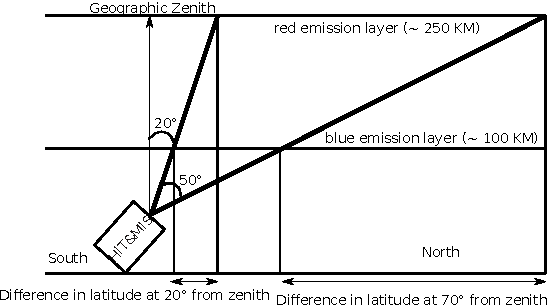
\includegraphics[width=35pc]{elayer.pdf}
	\caption{Viewing geometry of the HiT\&MIS instrument during the June 22-23, 2015 storm at Lowell, MA. The latitudes traced by the red and the blue lines are shown assuming the peak emission height of
		250 km and 100 km, respectively. Note that for measurements closer to the zenith the range of latitudes covered by each emission layer is small. However for measurements far away from the zenith, emissions from a larger latitude range are measured along the line of sight.}
	\label{fig:elayer1}
\end{figure}

During the observation period the sky was partly cloudy. The NeI (630.5 nm) emission feature (also observed by HiT\&MIS) which is produced by street lights is used as a tracer of cloud activity. Only periods with minimal cloud coverage are analyzed (see Figure \ref{feature:nbrg}). 

HiT\&MIS is capable of measuring six upper atmospheric 
emission features simultaneously at high spectral resolution ($\approx$ 0.02 nm at 630.0 nm).
 The bias frame was subtracted from each raw image (Figure \ref{fig:raw}A) but the dark frame was negligible ($\approx{}$ 0.0019 ADU $\rm s^{-1} pixel^{-1}$; red line intensity was $\approx$ 10-30 ADU $\rm s^{-1} pixel^{-1}$ for comparison) and hence ignored. Detailed description of steps taken for data reduction are described in Chapter 2. The brightness data from HiT\&MIS used for this work are available online at https://doi.org/10.5281/zenodo.1208111.
\begin{figure}[H]
	\centering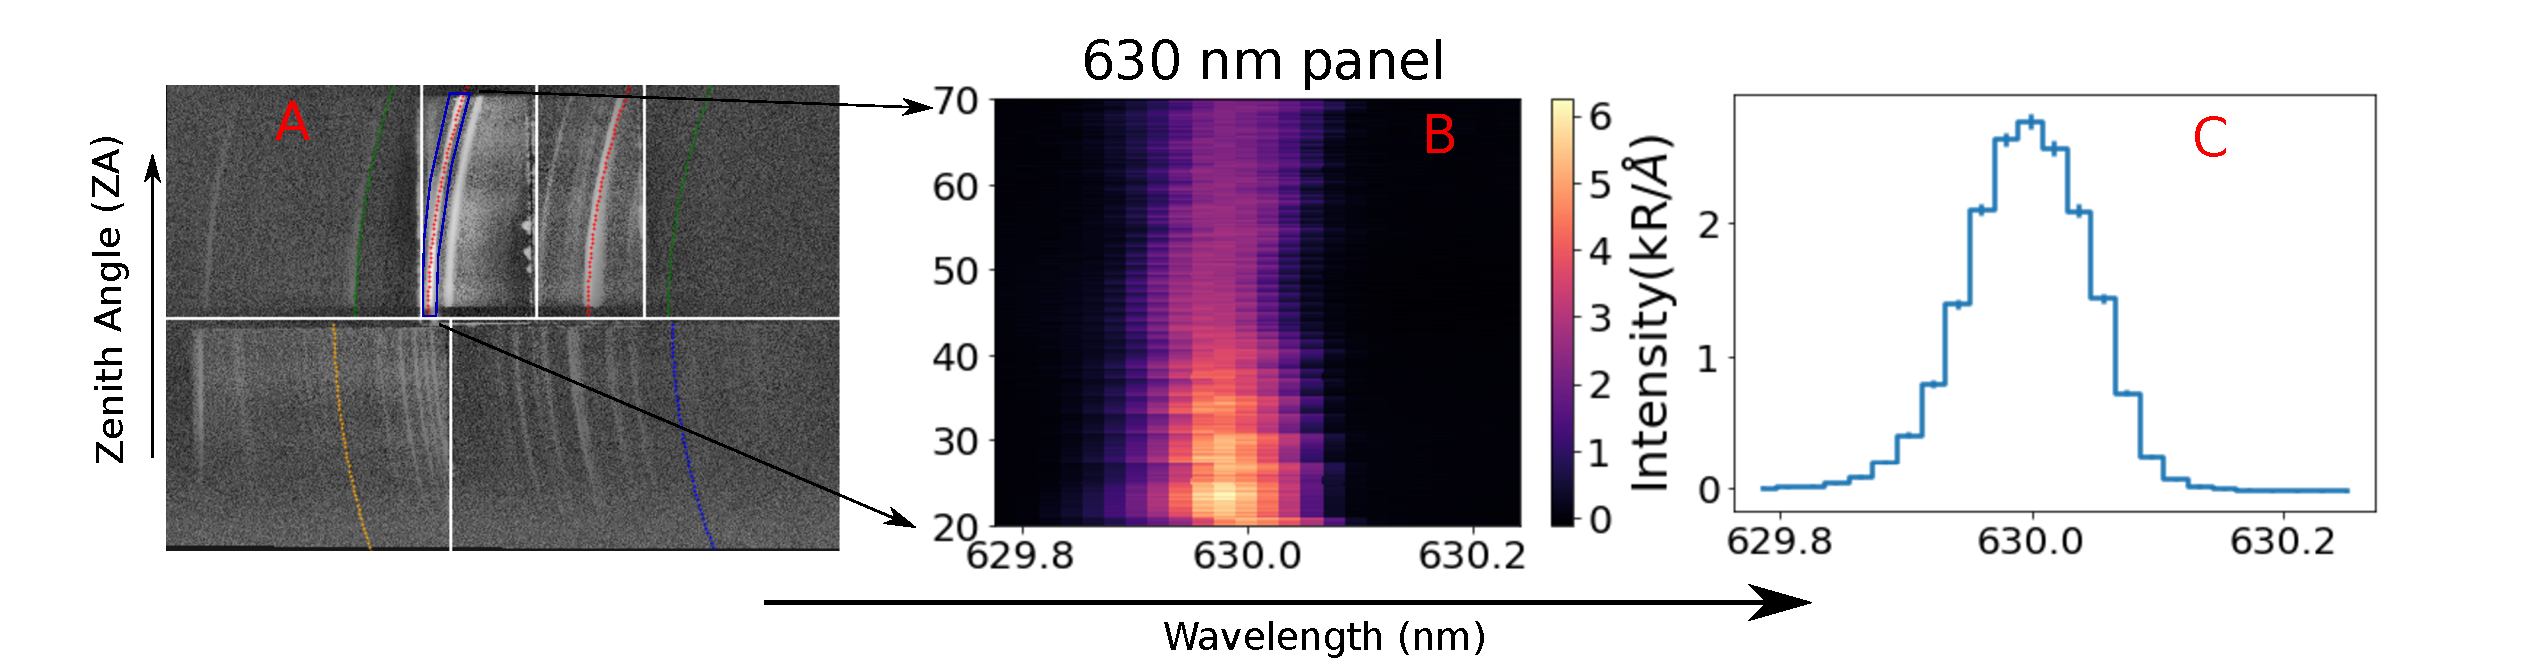
\includegraphics[width=35pc]{raw_spec.pdf}
	\caption{A: Sample raw image from HiT\&MIS at 22:30 PM LT on June 22, 2015 with 60 s exposure. Overlaid lines are the ray trace estimate of the line center locations of the emission features. B: Photometrically calibrated, background-subtracted 630.0 nm spectrum extracted from the region highlighted in A. C: Average spectrum obtained by integrating over 
		over the entire zenith angle range (y-axis in B) covered by HiT\&MIS.}
	\label{fig:raw}
\end{figure}


\subsection{Brightness Morphology} 
\label{sec:bmorph}
The brightness keograms of the red line, the green line, the blue line as a function of time and zenith angle is shown in Figure \ref{fig:brg}. To further assess the morphology of the emission as a function of time, the data was divided into three look directions (20-37$^\circ$, 37-54$^\circ$ and 54-70$^\circ$ zenith angles) and eight time ranges with minimal cloud coverage were selected for analysis (labeled T1-T8).
Figure \ref{feature:nbrg} shows the brightnesses for the three spectral features (plus the NeI cloud indicator) as a function of time at different look direction bins. During the time period T1, the brightness are lower at higher zenith angles for the all of the emission features. In contrast, during the time periods T3, T4 and T8 the red line brightnesses are higher at higher zenith angles (Figure \ref{feature:nbrg}). For these three cases, the brightnesses in the other features do not change significantly with change in zenith angle. The auroral red line emission occurs at higher altitude ($\approx$  250 km) and thus spans larger latitude ranges than the blue and green lines (Figure \ref{fig:elayer1}). Since this effect is larger for higher zenith angles (north, see Figure \ref{fig:elayer1}) we could have been looking at different auroral structure in red line for time periods T3, T4 and T8. 
This should have also been visible for the OI (777.4 nm) emissions as it peaks at even higher altitude, but it is not apparent in the poor signal to noise ratio data. 

In the time period T2, the red and the green line brightnesses were relatively constant with time and zenith angles but a few small peaks can be seen in the blue line brightness (see T2 in Figure \ref{feature:nbrg}), particularly at the 37-54$^\circ$ zenith angle look direction. 
There was a decrease in the red line brightness during time period T5, with a few small peaks in the green and blue lines. During the time period T6, all the emission brightnesses were increasing with time, but the increase in the red line was more prominent than other features. These different temporal and angular morphologies in brightnesses provide an opportunity to examine their implications on energies and fluxes are discussed in section \ref{sec:emorph}. These average brightnesses were the measured data points used for energy and flux derivation for their particular look directions bins (see Figure \ref{feature:nbrg}). This thesis describes the methods we used to study the feasibility of estimating energies and energy fluxes during the time intervals T1 through T8 in Figure \ref{feature:nbrg} for three look directions. 

%Since the peak emission height of each of the features is different, the measurements represent different latitudes as shown in Figure \ref{fig:elayer1} (do we need this part?).

%%%%
%%%%%%
\begin{figure}[H]
	\centering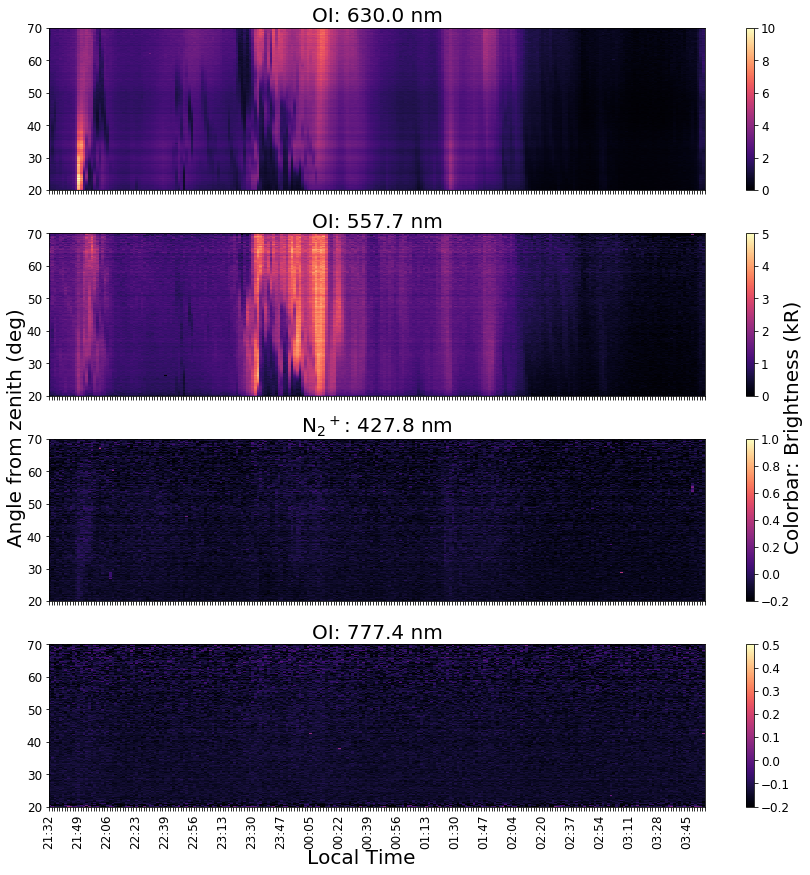
\includegraphics[width=35pc]{brg_night.png}
	\caption{Brightness keogram of the four emissions observed with HiT\&MIS through the night of June 22-23, 2015 at different zenith angles and times with 60s exposure time. This keogram was used to select the three features to obtain energy and flux information.
		The emission lines have offsets added to them for clarity. For example, the the green line emission brightness values have an offset of 2 added. The $\pm$1$\sigma$ uncertainties are shown as vertical error bars, which are most prominently seen in the blue line emission brightness.
		The times with minimal cloud activity chosen for analysis are shown with dashed vertical lines and labeled T1 through T8.}
	\label{feature:brg}
\end{figure}

\begin{figure}[H]
	\centering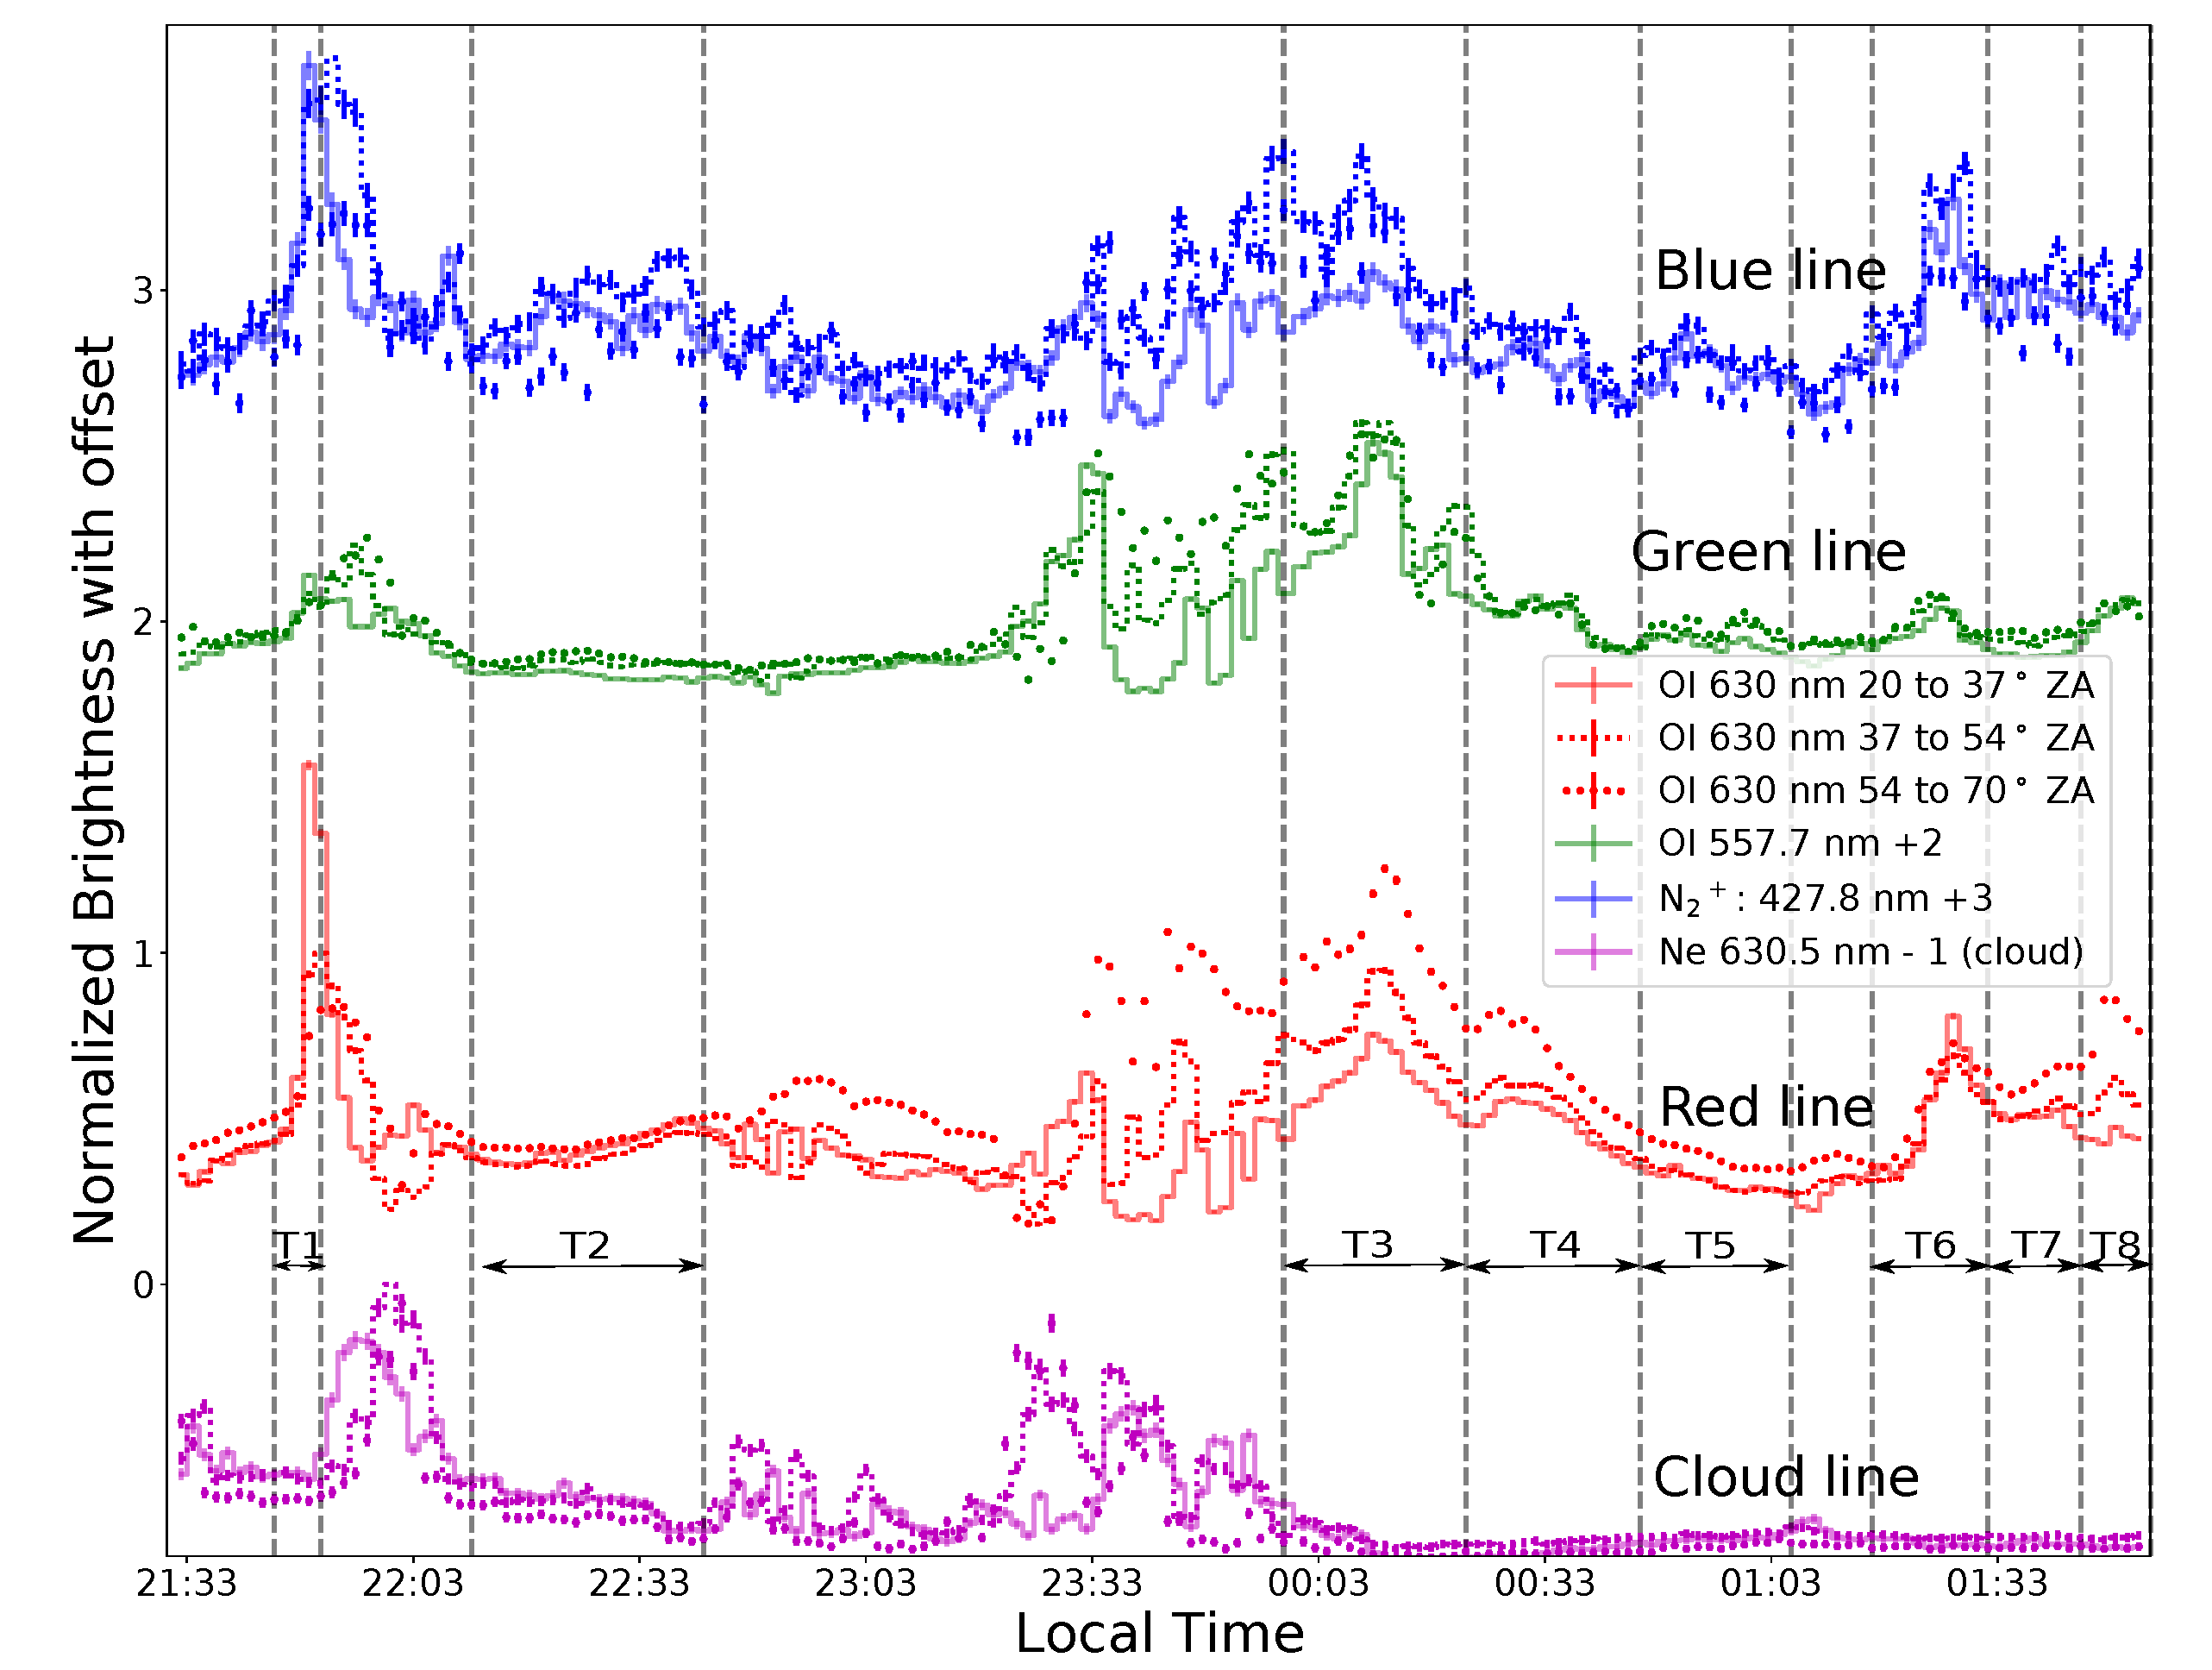
\includegraphics[width=35pc]{nbgr.pdf}
	\caption{Normalized brightness of the four emissions observed with HiT\&MIS through the night of June 22-23, 2015 obtained by averaging along: 20 to 37$^\circ$ (solid line), 37 to 54$^\circ$ (dashed line) and 54 to 70$^\circ$ (dotted line) zenith angles with 60s exposure time. The Ne I (630.5 nm) emissions, used as proxy for cloud activity, is shown in magenta.  
		The emission lines have offsets added to them for clarity. For example, the the green line emission brightness values have an offset of 2 added. The $\pm$1$\sigma$ uncertainties are shown as vertical error bars, which are most prominently seen in the blue line emission brightness.
		The times with minimal cloud activity chosen for analysis are shown with dashed vertical lines and labeled T1 through T8.}
	\label{feature:nbrg}
\end{figure}

\section{Modeling} 
\label{sec:model}
The GLOW model is based on a two stream electron transport method of \citet{nagybanks1970}. The precipitating electrons were assumed to have a Maxwellian energy distribution with a characteristic energy ($E_{0}$) and total energy flux ($Q_{0}$). These primary electrons then interact with neutral atmospheric species provided by the climatological neutral atmospheric model, NRLMSIS00 (Naval Research Laboratory Mass Spectrometer Incoherent Scatter 2000) \citep{msie} as they move through the upper atmosphere. The climatological ionospheric model, IRI-90 (International Reference Ionosphere 1990) \citep{iri} provides the electron and ion densities and temperatures for photochemical calculations.

 The altitude profiles for the volume emission rate (VER) of the observed emission features were modeled for different input characteristic energies and fluxes using the GLOW model (Figure \ref{fig:vve}, \ref{fig:bve}). 
We vary the energy and flux inputs into GLOW and integrate along line of sight volume emission rate (VER, Figure \ref{fig:vve}) to estimate brightness. Brightnesses for the red line, green line, blue line and the OI 777.4 nm emissions as a function of different energies and fluxes are presented in Figure \ref{fig:bve}. Notice that while all the brightnesses increase with increasing flux, brightnesses for each emission peak around particular energies for different emissions.
\begin{figure}[H]
	\centering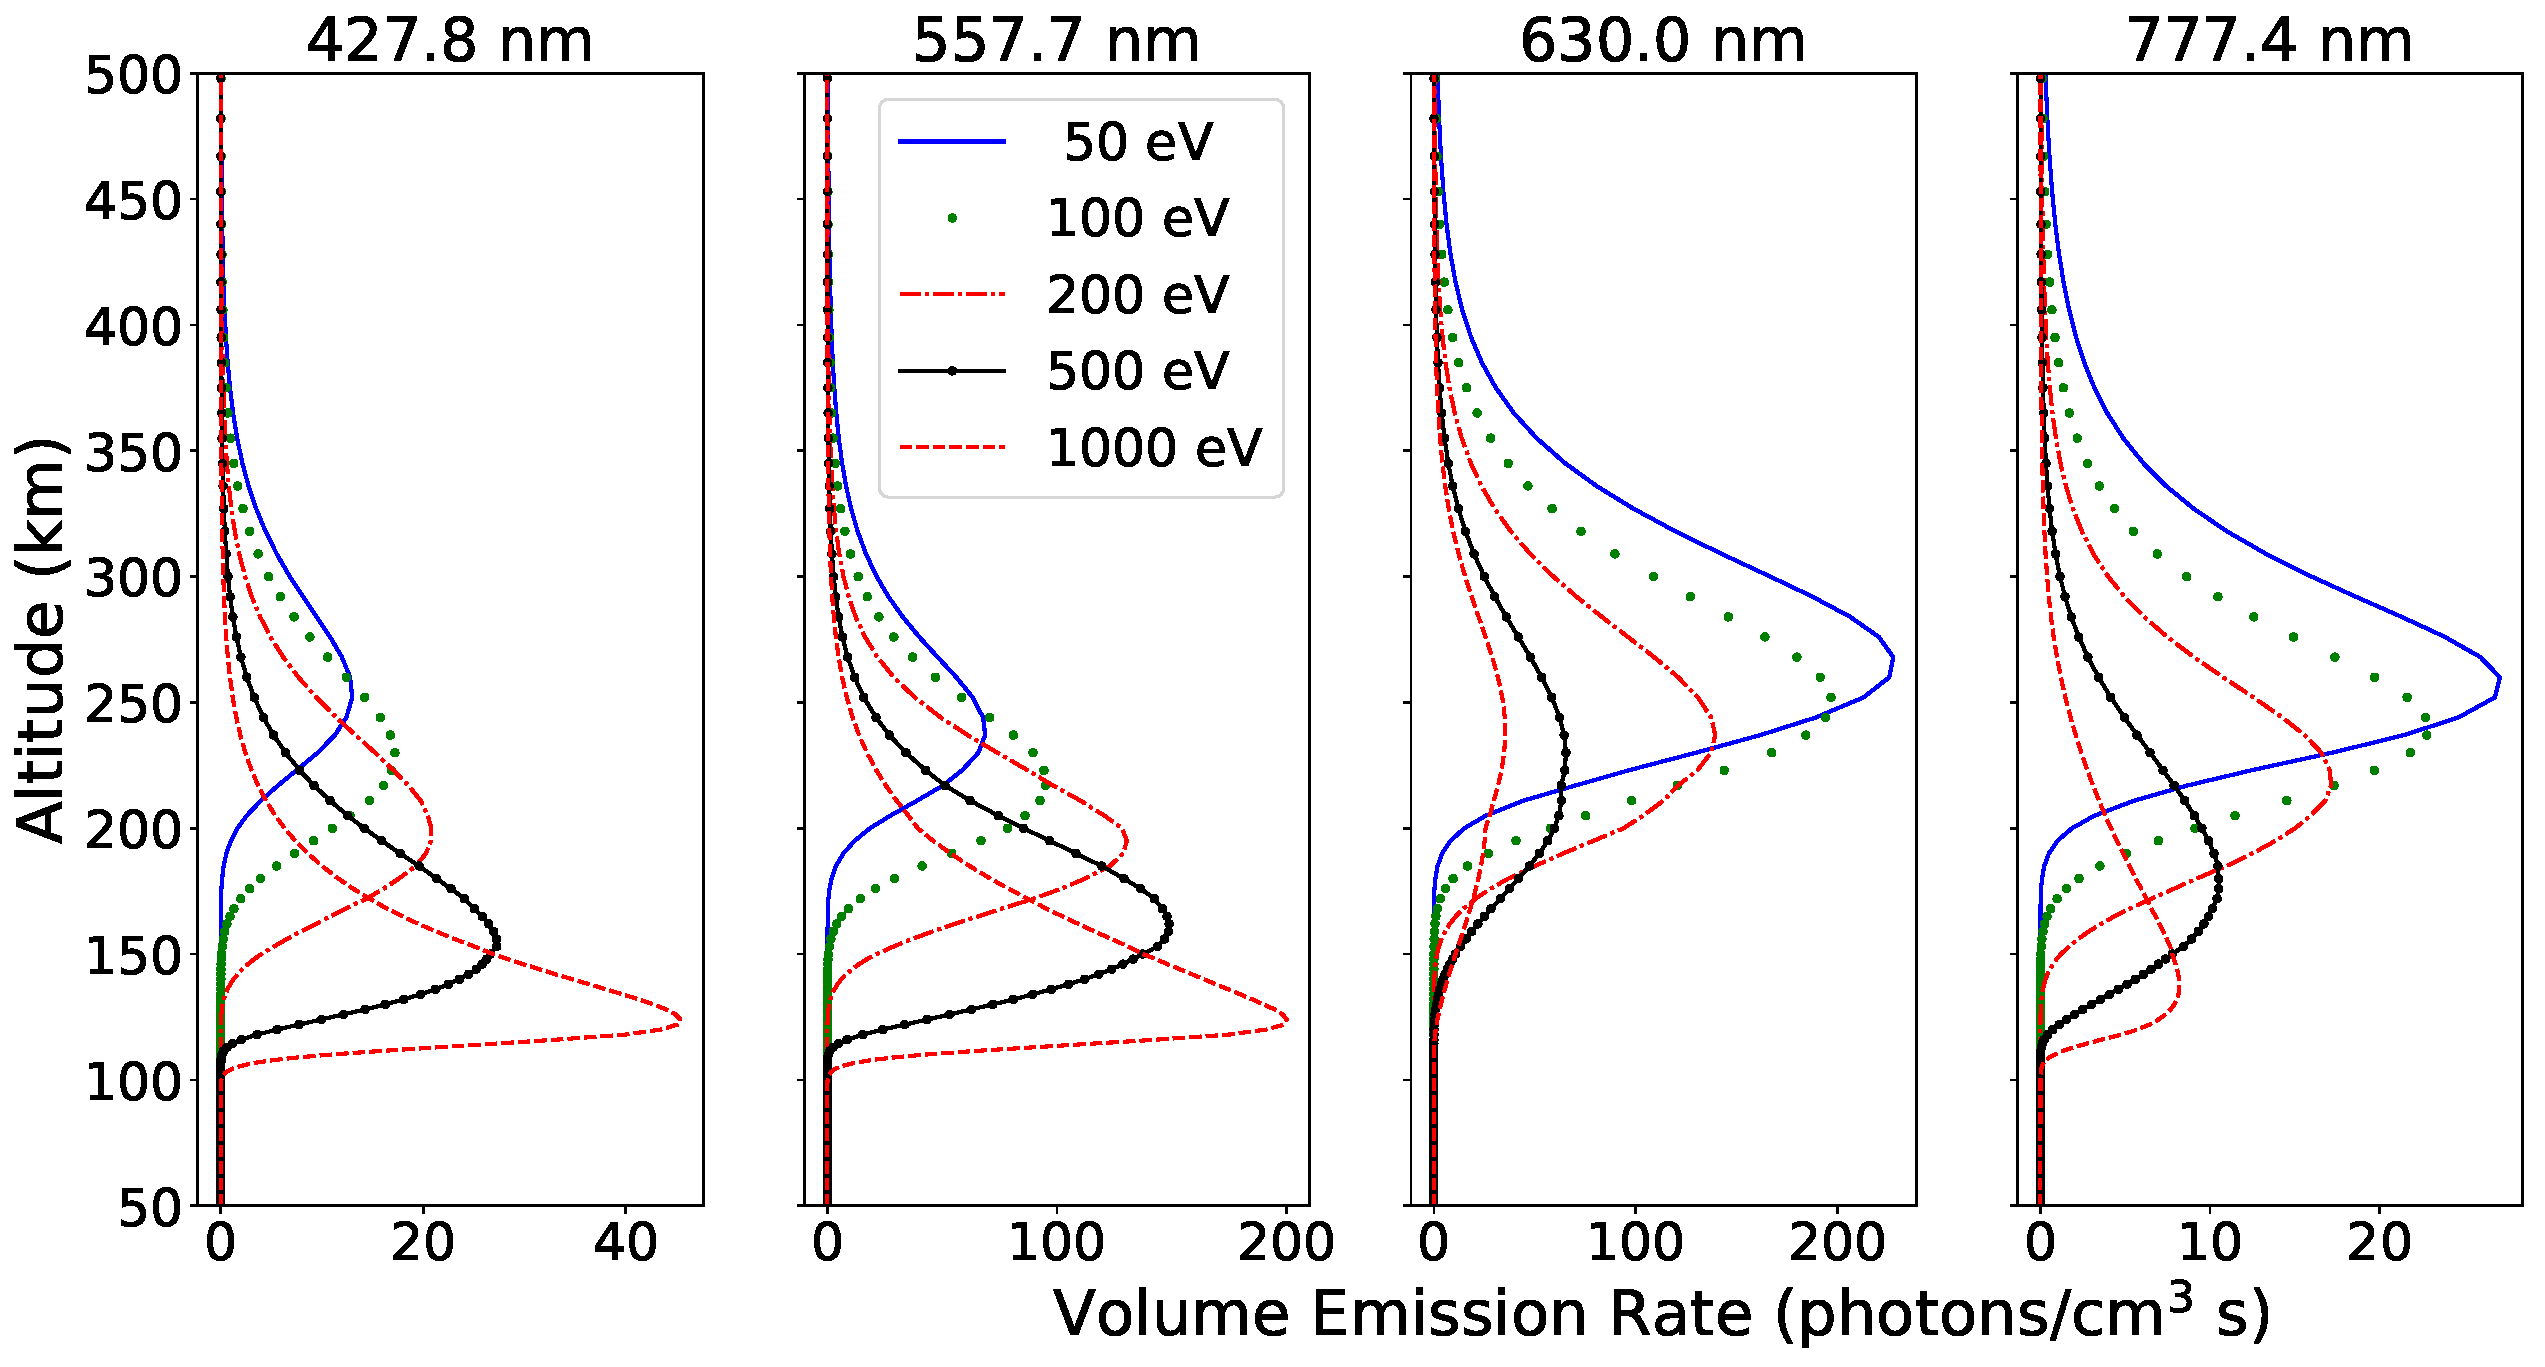
\includegraphics[width=35pc]{ver_vs_e.pdf}
	\caption{GLOW model volume emission rates with varying energy and a constant flux of 1 erg $\rm cm^{-2}$ $\rm s^{-1}$ computed for the four emission features. Auroral contribution to VER is linearly proportional to flux. Note the peak VER and the altitude of the peak change differently for the different features as a function of energy. For
		example, the peak height for red line (630.0 nm) is around 250 km for all energies and peak VER occurs at less that 100 eV, while the for the blue line (427.8 nm) the peak height is around 100 km and the peak VER occurs in the 1 keV range.}
	\label{fig:vve}
\end{figure}
\begin{figure}[H]
	\centering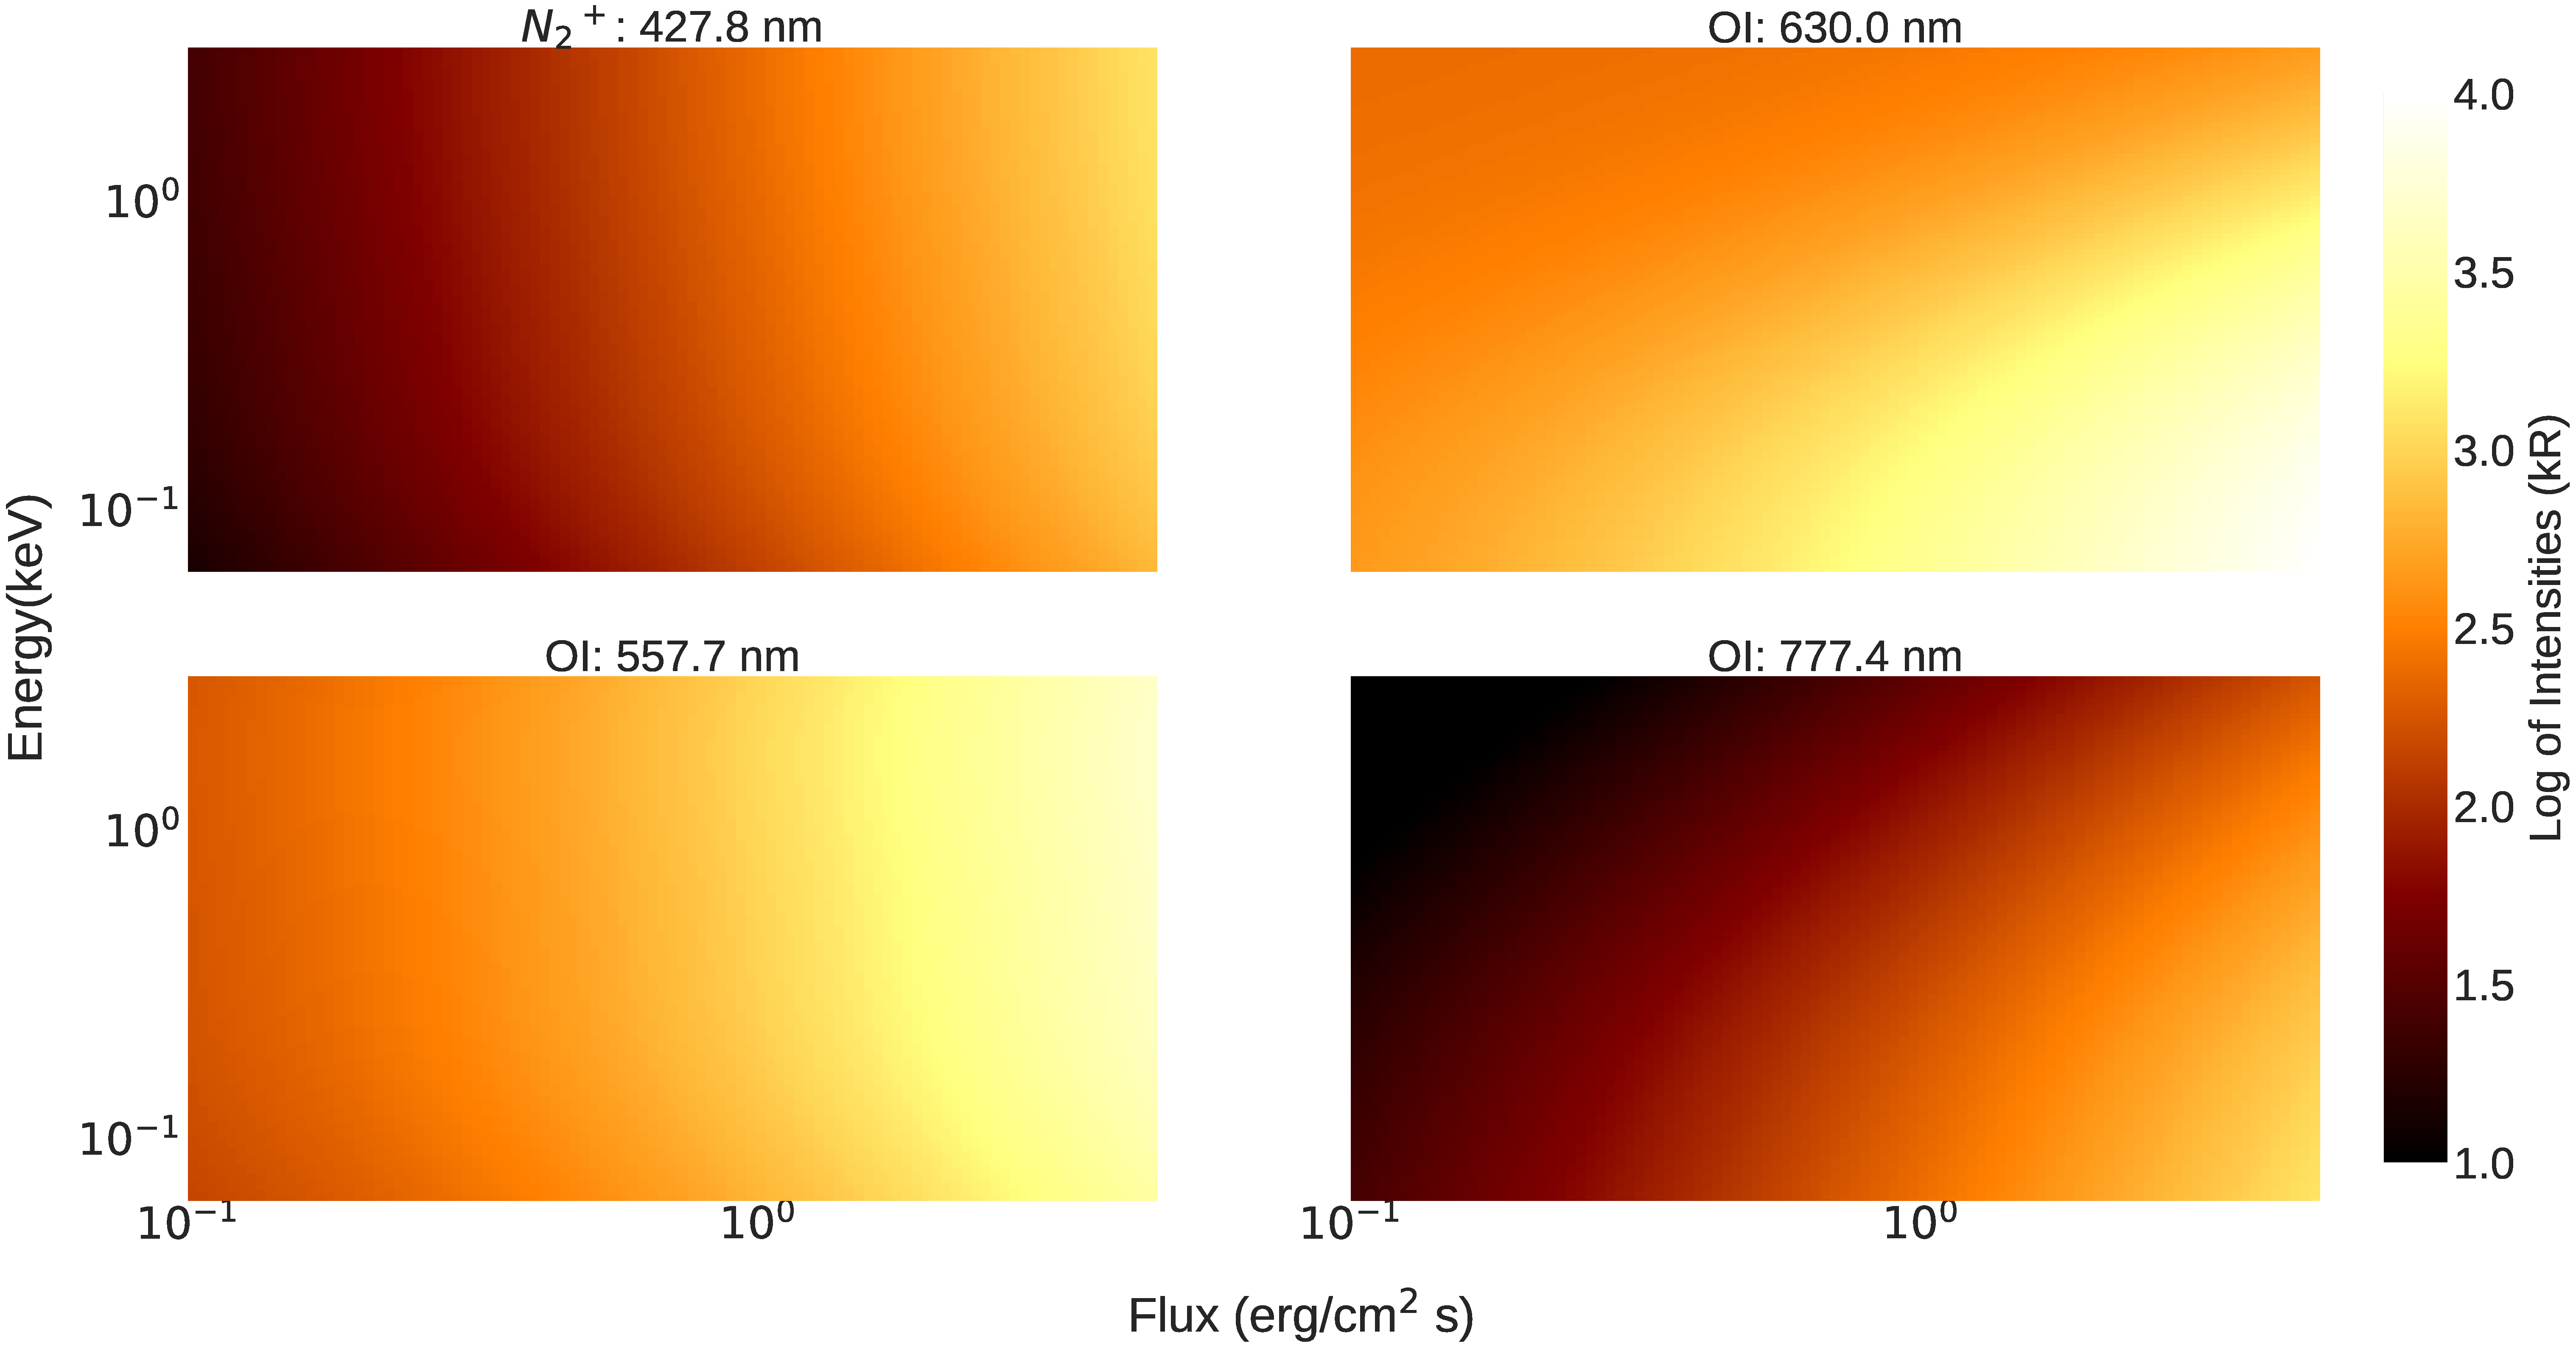
\includegraphics[width=35pc]{b_vs_e.pdf}
	\caption{Line of sight brightnesses as a function of characteristic energy and energy flux as predicted by GLOW at 9:50 PM on June 23 using IRI-90 and NRLMSIS00 ion and neutral parameters, respectively.}
	\label{fig:bve}
\end{figure}
\subsection{Fluorescence contribution removal}
The output of the GLOW model showed two peaks in the blue line VER profile, one at higher altitude and the other at lower altitude. The emission peak at the higher altitude was due to resonance fluorescence of $N{_2}{^+}$ by solar radiation. Because all of the observation are during nighttime, this contribution due to fluorescence is subtracted in each model run (including Figure \ref{fig:vve}). This contribution was removed by subtracting the fluorescence contribution to the $N{_2}{^+}$ (427.8 nm) VER profile for each of our model runs. Figure \ref{fig:fl_rmv} shows, the blue line brightness as predicted by the glow model with and without the resonance fluorescence contribution.
\begin{figure}[H]
	\centering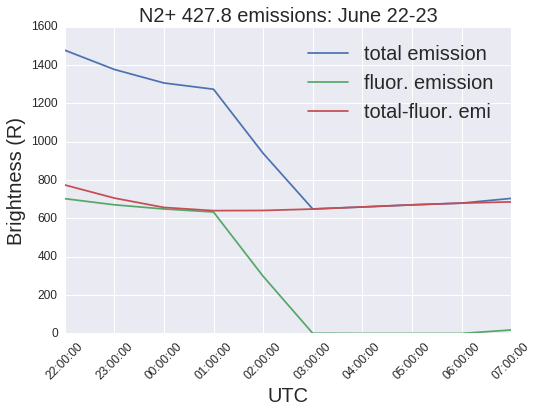
\includegraphics[width=35pc]{flu_cont_rmv.png}
	\caption{GLOW model blue line brightnesses with and without the resonance fluorescence contribution.}
	\label{fig:fl_rmv}
\end{figure}

%%%%%%%%
% \begin{figure}
% \centering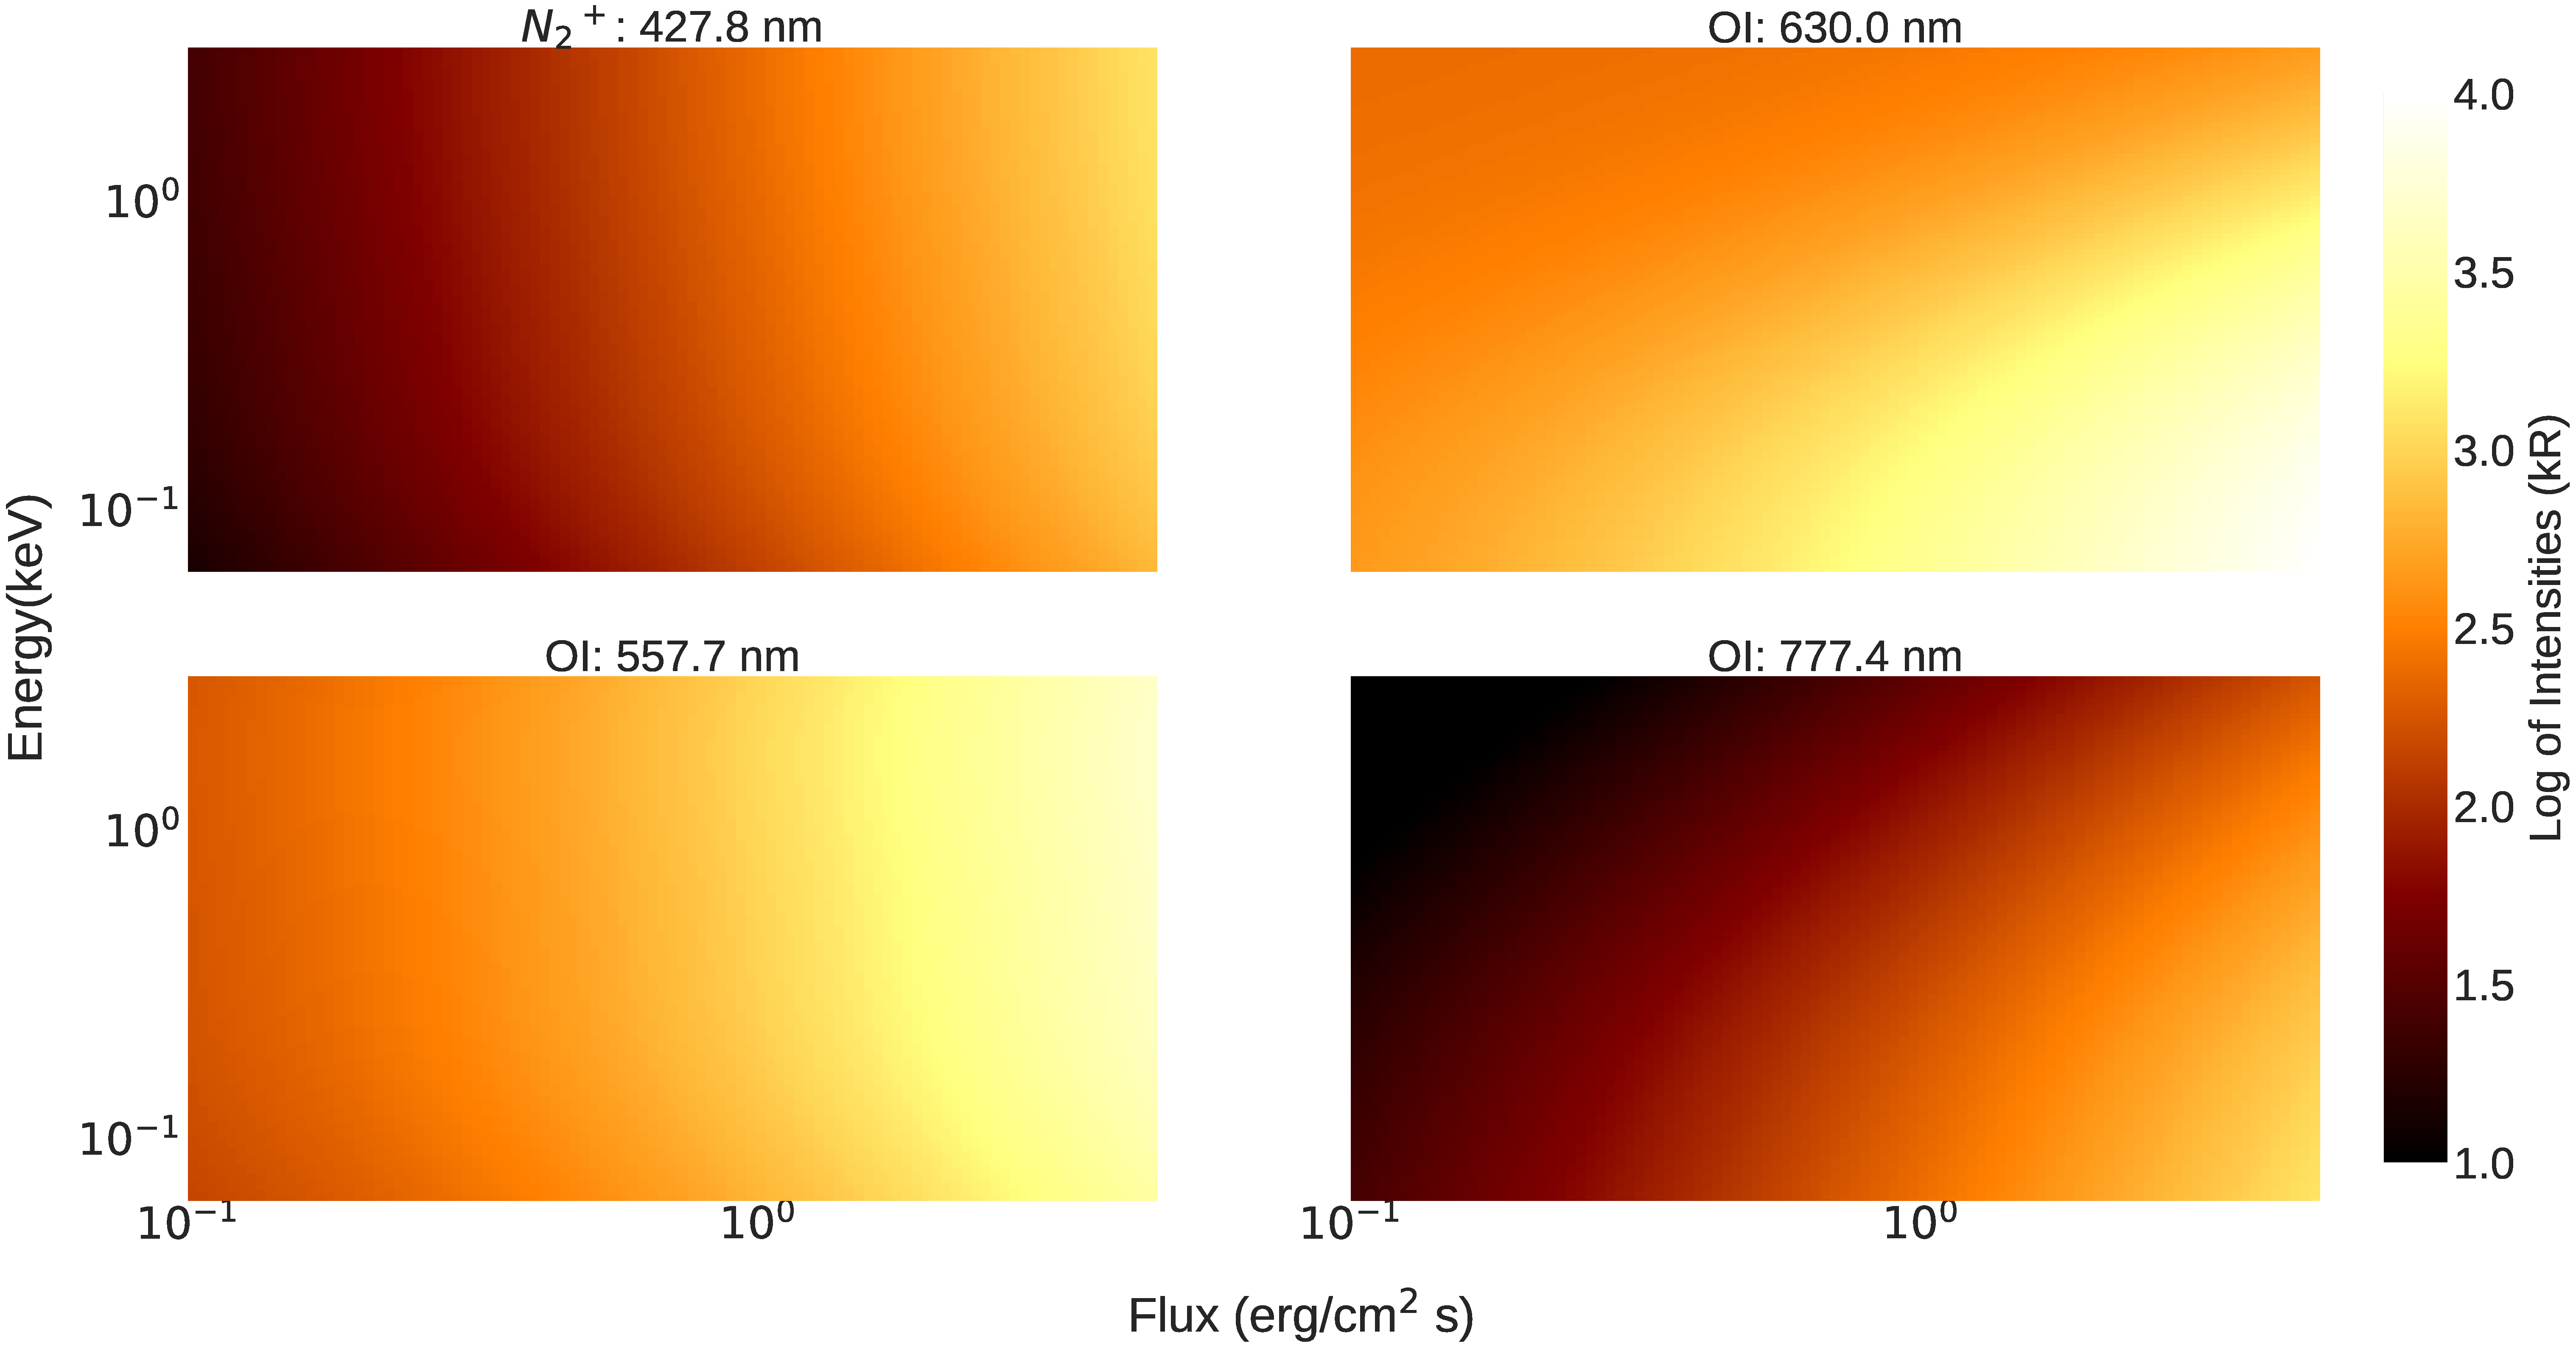
\includegraphics[width=30pc]{b_vs_e.pdf}
% \caption{Line of sight brightnesses as a function of characteristic energy and energy flux as predicted by GLOW at 9:50 PM on June 23 using IRI-90 and NRLMSIS00 ion and neutral parameters, respectively.}
% \label{fig:bve}
% \end{figure}
%\begin{figure}
% \centering\includegraphics[width=30pc]{b_e_f_r.eps}
% \caption{Brightness ratios as a function of energy and energy flux for the selected features}
% \label{fig:chi}
% \end{figure}
%%%%%%%%%%%%%%%%%%%%%%%%%%
\section{Energy and Flux derivation from optical emissions}
\subsection{Motivation for method selection}
The hmF2 is sensitive to changes in energy of the precipitating electrons because this determines where the electrons are stopped \citep{rees_1963}. \cite{pallamraju_2011} used this concept to derive the energy of precipitating electrons. 
% \begin{figure}[H]
% 	\centering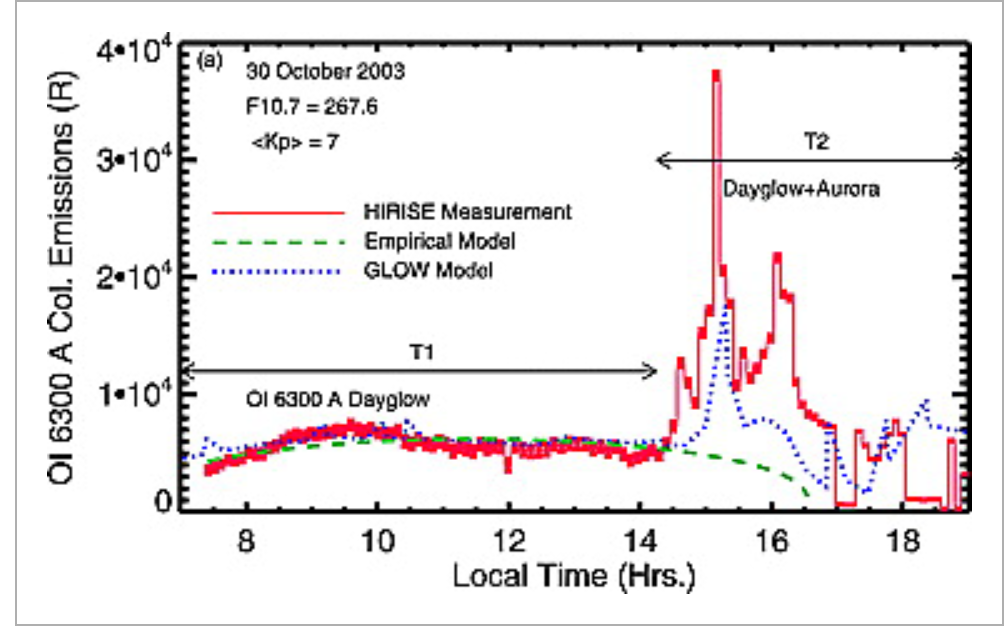
\includegraphics[width=35pc]{pall_r_glow.png}
% 	\caption{HIRISE red line measurement during an auroral event over Boston, MA on 30 October, 2003. GLOW model estimate for the same event with a fixed flux. From \cite{pallamraju_2011}. }
% 	\label{fig:plm_gl}
% \end{figure}
% \begin{figure}[H]
% 	\centering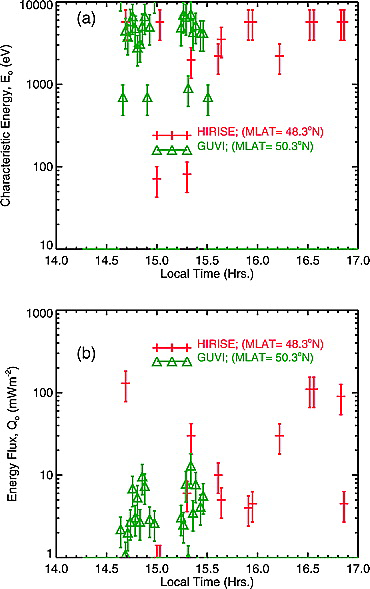
\includegraphics[width=25pc]{e_fl_plm.png}
% 	\caption{Energy and flux derived by \cite{pallamraju_2011}, and its comparison with energy and flux derived by an UV instrument close to the same magnitude latitude.}
% 	\label{fig:plm_efl}
% \end{figure}
% \begin{figure}[H]
% 	\centering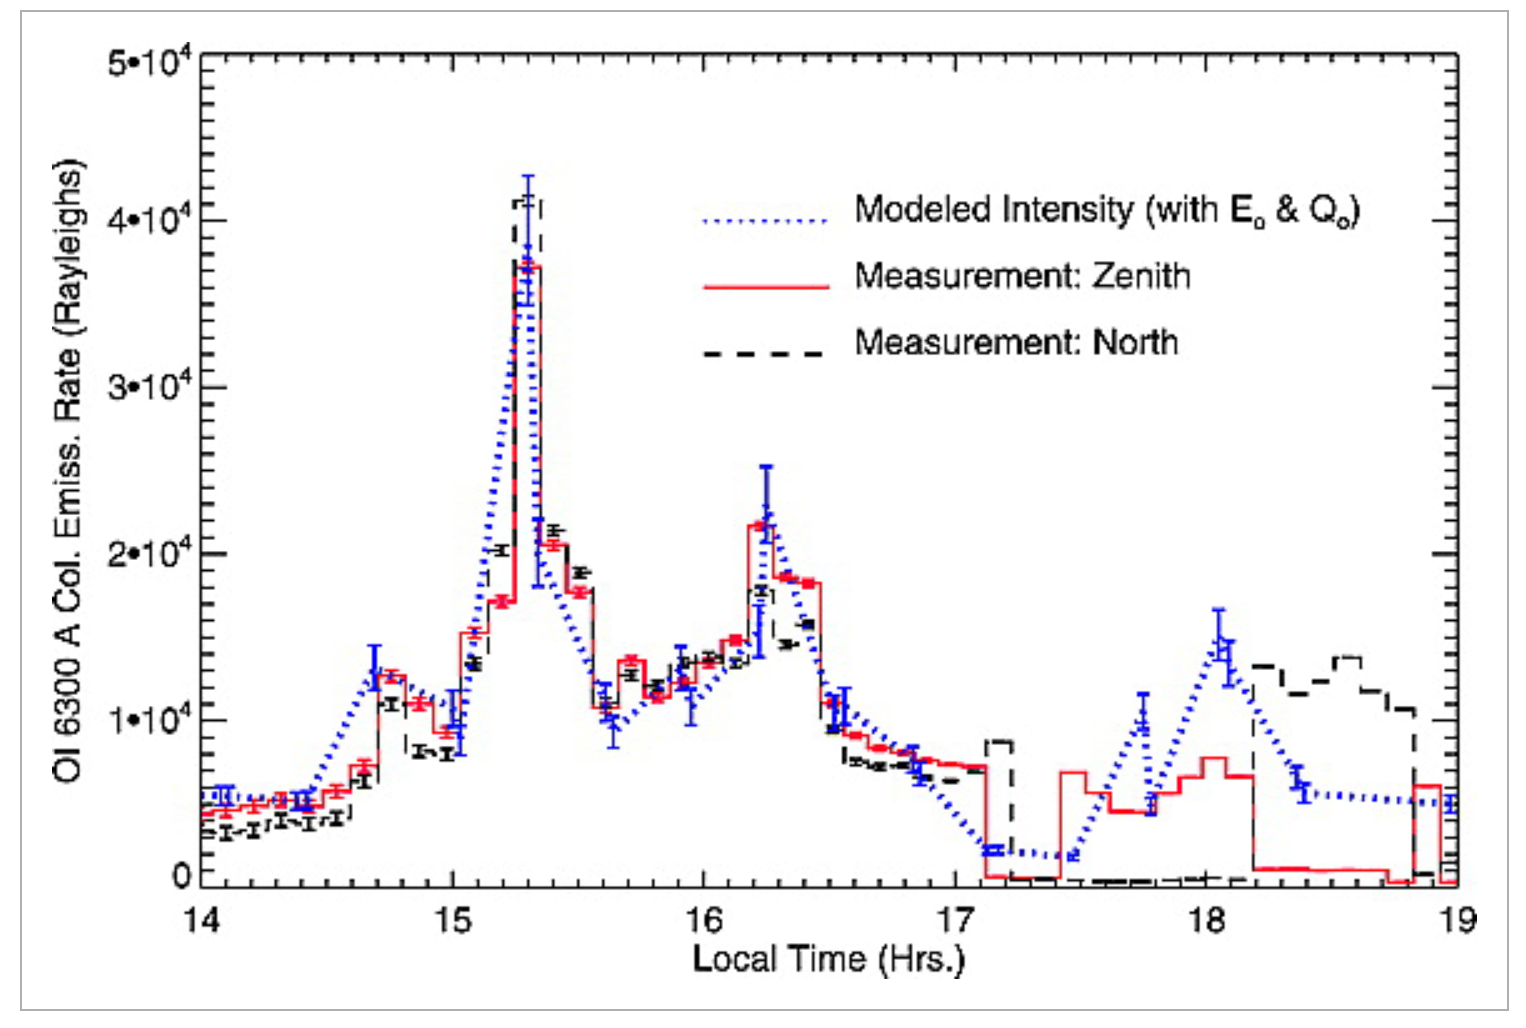
\includegraphics[width=35pc]{palam_retrv.png}
% 	\caption{Comparison between GLOW model red line brightness using energies and fluxes derived in Figure \ref{plm_elf} and HIRISE measurement. From \cite{pallamraju_2011}.}
% 	\label{fig:plm_gl}
% \end{figure}

Similarly, \cite{rees_1974} utilize red to blue line brightness ratios to infer the energy of the precipitating electrons. The red line emission peaks at higher altitudes and the blue line peaks at lower altitudes making them more sensitive to low and high energy electrons, respectively (Figure \ref{fig:vve}). Thus, their brightness ratio is sensitive to the energy of precipitating electrons. Also, as all the brightnesses increase with flux, \cite{pallamraju_2011} and \cite{rees_1963} use the red and the blue brightnesses, respectively, to estimate the flux. In addition, \citet{grubbs_compare} use the OI 844.6 to green line ratio and the blue line brightness in conjunction with a modified version of the GLOW model to derive energy and flux during an auroral event. Like the red line, the OI 844.6 nm emission peaks at higher altitude and is more sensitive to low energy electrons. \citet{grubbs_compare} compared the energy and flux derived using the optical method in situ particle measurements and found good correlation within 20$^\circ$ of magnetic zenith.

For our study, we explore whether or not the brightnesses or the brightness ratios of the three auroral features alone can be used to simultaneously derive both energy and fluxes. This was done by comparing the simultaneously derived energies and fluxes with a hybrid method using ratios to infer energy and then brightnesses to infer fluxes for comparison. 



\subsection{Methods}
Three different methods, summarized in Table \ref{table:method}, were used to derive electron energies and fluxes for the June 22-23, 2015 aurora. 
All of the methods were based on the iterative non-linear minimization of chi-square ($\chi^2$, weighted least-squares) at each observation time, t:


\begin{equation}
\large
\chi^{2}_t (E,Q) = \sum_{i}\Bigg({\frac{O_{i} - M_{i} (E,Q)} {\sigma_{i}}}\Bigg)^{2}.
% +({\frac{O_{557} - M_{557}} {\sigma_{557}}})^2+({\frac{O_{427} - M_{427}} {\sigma_{427}}})^2+({\frac{O_{777} - M_{777}} {\sigma_{777}}})^2
\label{eq:chi}
\end{equation}
Here, at time t, $O_{i}$ and $M_{i}$ are the observed and modeled brightnesses (or brightness ratios) of $ i^{th}$ emission feature, respectively, and $\sigma_{i}$ represents the standard deviation (in brightness) of the $ i^{th}$ emission feature. Figure \ref{chi_eo} shows an example of $\chi^2$ surface using emission brightnesses at 10:30 PM LT on June 21, 2017; a rough estimate of energy and flux at this time is also shown. For robust calculations, energy ($E$) and flux ($Q$) are input into the GLOW model and are iteratively varied to minimize $\chi^2$ (Equation \ref{eq:chi}) using the Levenberg-Marquardt algorithm (LMA) \citep{levenberg,marquardt}. LMA is based on a combination of gradient descent (towards minimum) and residual (in our case $\chi^2$, the weighted squared residual) minimization methods. The covariance matrix returned by this method gives us the statistical uncertainties in the derived parameters which were taken to be the final uncertainties since the model uncertainties are not considered. 
\begin{figure}[H]
	\centering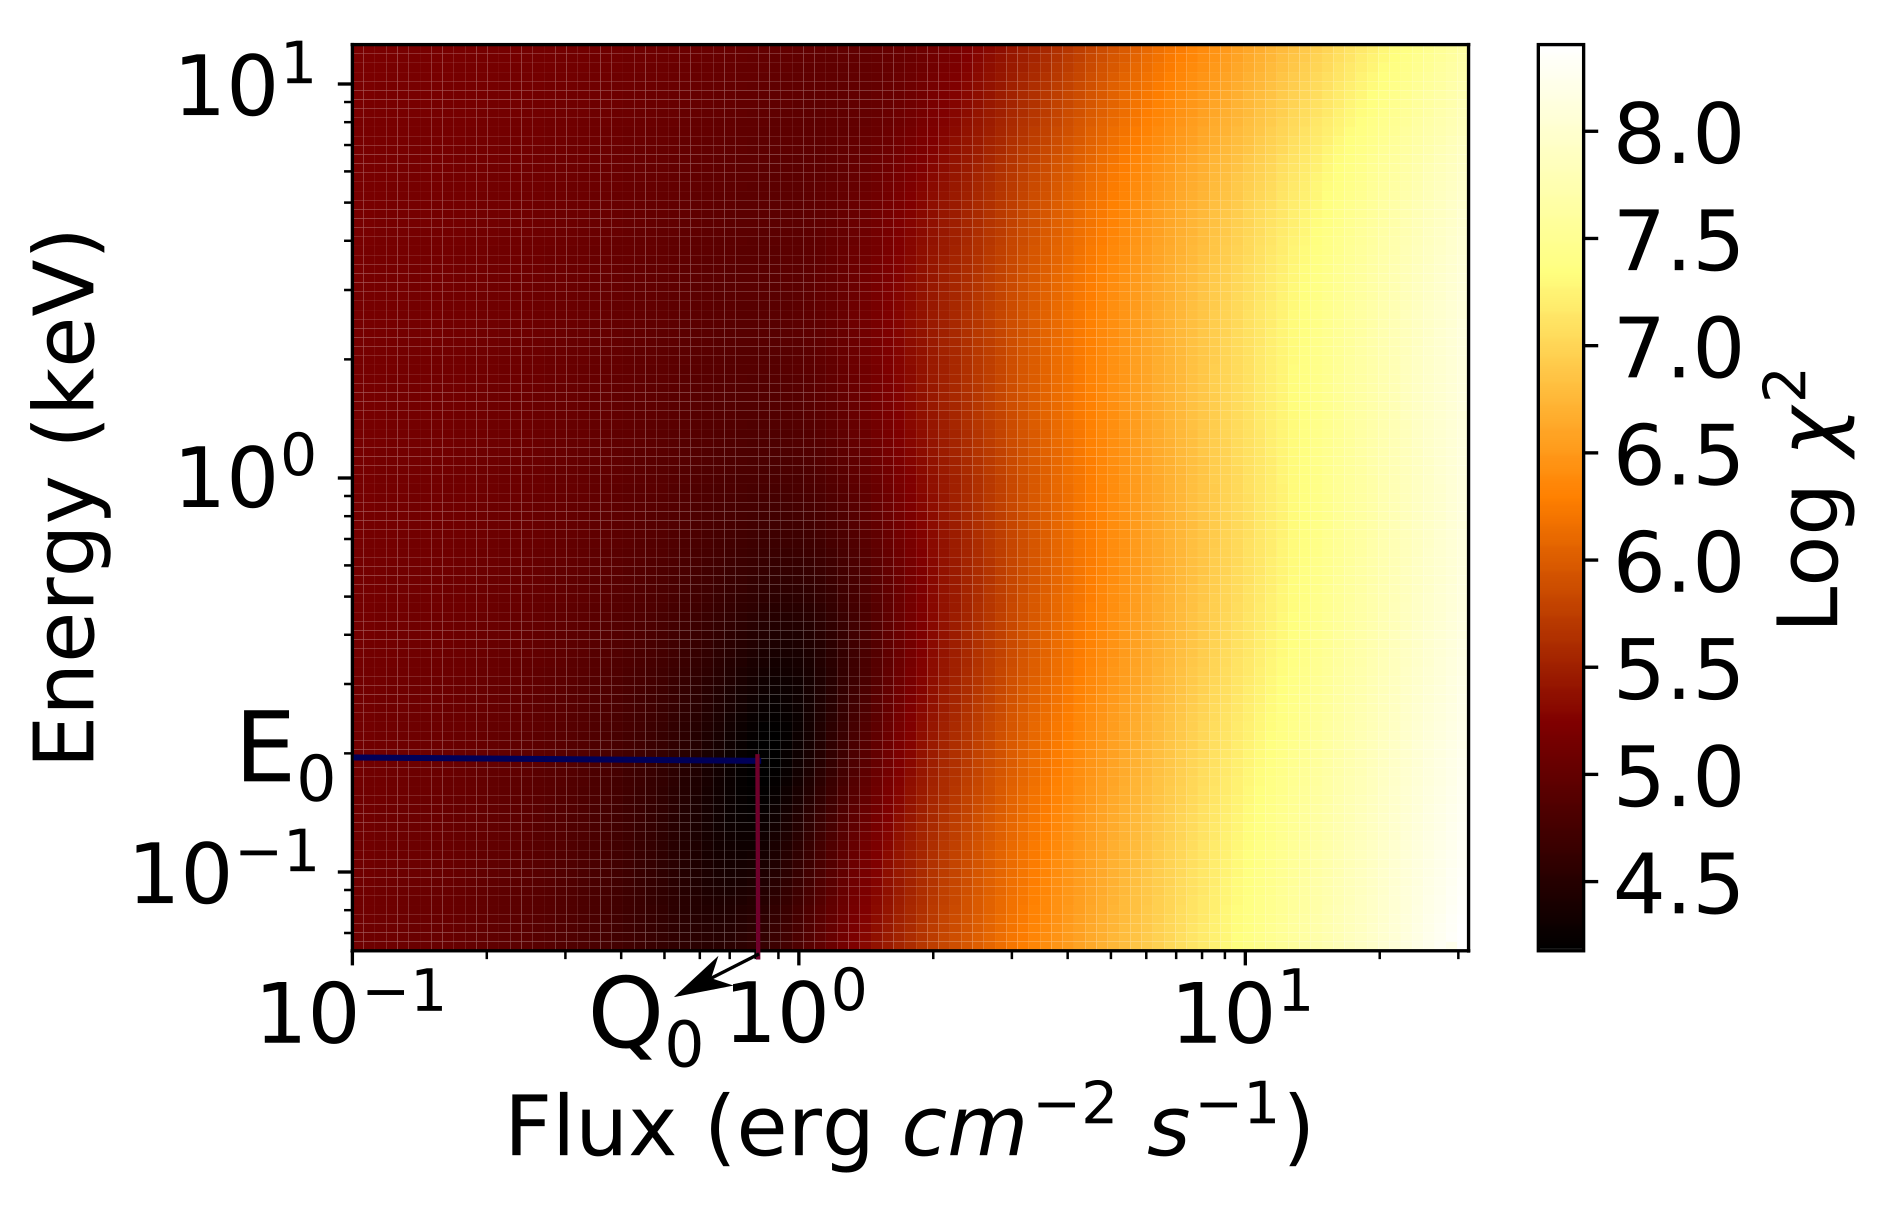
\includegraphics[width=35pc]{chi_eo.png}
	\caption{ $\chi^2$ as a function of energy and flux input into the GLOW model.}
	\label{fig:chi_eo}
\end{figure}

The three methods mentioned below are applied to derive energy and flux (summarized in Table \ref{table:method}) by performing the non-linear minimizations using the $LMFIT$ module for Python \citep{lmfit}. The characteristic energy of the Maxwellian distribution, $E_0$, as discussed in section \ref{sec:model} is being reported. For a Maxwellian distribution, to convert to average energy ($E_{av}$), $E_0$ can be multiplied by a scaling factor, i.e., $E_{av}$ = 2 $E_0$ \citep{kosch_2001}.
\subsubsection{Brightness method}
\label{sec:brightness}
In this method, the modeled brightnesses in red, green and blue lines were compared with the measurements by simultaneously varying $E$ and $Q$ inputs into the GLOW model to minimize $\rm \chi^2$. This method explores the feasibility of directly comparing model with the measurements to derive energies and fluxes of auroral electron precipitation.

\subsubsection{Ratio method}
\label{sec:ratio}
In this method, the modeled ratios of blue to red, blue to green and green to red lines were compared with the measured ratios to derive energies and fluxes of precipitating electrons. This was done in similar fashion as the brightness method (section \ref{sec:brightness}) by varying $E$ and $Q$ simultaneously to minimize $\rm \chi^2$. 

\subsubsection{Hybrid method}
\label{sec:2step}

%\cite{rees_1963}. Then, the energy fluxes were estimated by varying flux input to the GLOW model until the model matched the measured red line brightness at the derived energy.
This method is similar to that used by \cite{pallamraju_2011} where energies and fluxes were derived using two steps.\cite{pallamraju_2011} had only the red line brightness measurements and so used the electron density profile ($N_e$) from ISR measurements to derive energies of the precipitating electrons. GLOW model red line brightness (at the derived energies) were then constrained with measurements to derive energy fluxes. Since we have simultaneous measurements of three emission features, we used the brightness ratios to predict the energies following a method similar to \cite{rees_1974} and then used the brightnesses to derive fluxes. First, the modeled brightness ratios of the blue to red, blue to green and red to green lines were compared with the measured brightness ratios to derive energies. This was done by varying $E$ to minimize $\rm \chi^2$ while $Q$ was kept constant at 1 erg $\rm cm^{-2} s^{-1}$. Then, at the derived energy ($E_0$), $Q$ was varied in the GLOW model to minimize $\rm \chi^2$ to compare the model brightnesses of red and green lines with the measured brightnesses. 


\begin{sidewaystable}
	
	\caption{Summary of the three different methods used to minimize $\chi^2$ in Equation \ref{eq:chi}.}
	\begin{tabular}{|l|l|}
		\hline
		
		Method &  Approach \\
		\hline
		\centering
		Brightness & \makecell{Constrain $E$ and $Q$ simultaneously\\ by comparing model brightness with measurements}\\ 
		
		\hline
		Ratio  &  \makecell{Constrain $E$ and $Q$ simultaneously\\ by comparing modeled brightness ratios with measurements}\\
		\hline
		
		Hybrid & \makecell{Step 1: Keep $Q$ constant and constrain $E$\\
			by comparing model brightness ratios with measurements\\
			\hline			
			Step 2: At $E$ derived in Step 1, constrain $Q$\\
			by comparing model brightness with measurements}\\
		\hline
	\end{tabular}
	\label{table:method}
\end{sidewaystable}
\section{Results}
Figure \ref{fig:e_fl_3mtd} shows the results derived using these methods for one selected look direction (37-54$^\circ$ ZA). The results are similar for other look directions. The hybrid method produced the least uncertainties in the derived energies and fluxes given by the minimization routine (Figure \ref{fig:e_fl_3mtd}). However, for flux derivation the uncertainties in the derived energies cannot be propagated without modifying the GLOW model. Using the upper and lower energy limits of the derived energy as input into the GLOW model, the difference in derived fluxes, assumed to be the estimated uncertainty in fluxes due to the uncertainty in energies, were found to be insignificant (in the range of $\approx$ $\pm$0.01 erg $\rm cm^{-2} s^{-1}$). Also, as mentioned in section \ref{sec:2step}, the hybrid method uses a constant flux input into the GLOW model during the first step to derive energies. We varied the initial flux estimates from 0.1 erg $\rm cm^{-2} s^{-1}$ to 50 erg $\rm cm^{-2} s^{-1}$ and found that the derived results did not vary significantly for flux values greater than 0.1 erg $\rm cm^{-2} s^{-1}$ (Figure \ref{fig:fl_d}). The derived energies for this method ranged from 57 eV to 278 eV while the flux ranged from 0.8 to 2.8 erg $\rm cm^{-2} s^{-1}$. This method also produced the best match between the measured red and green line brightnesses and the model estimates with the derived energies and fluxes as inputs into GLOW (Figure \ref{fig:e_fl_b_comp}).
\begin{figure}[H]
	\centering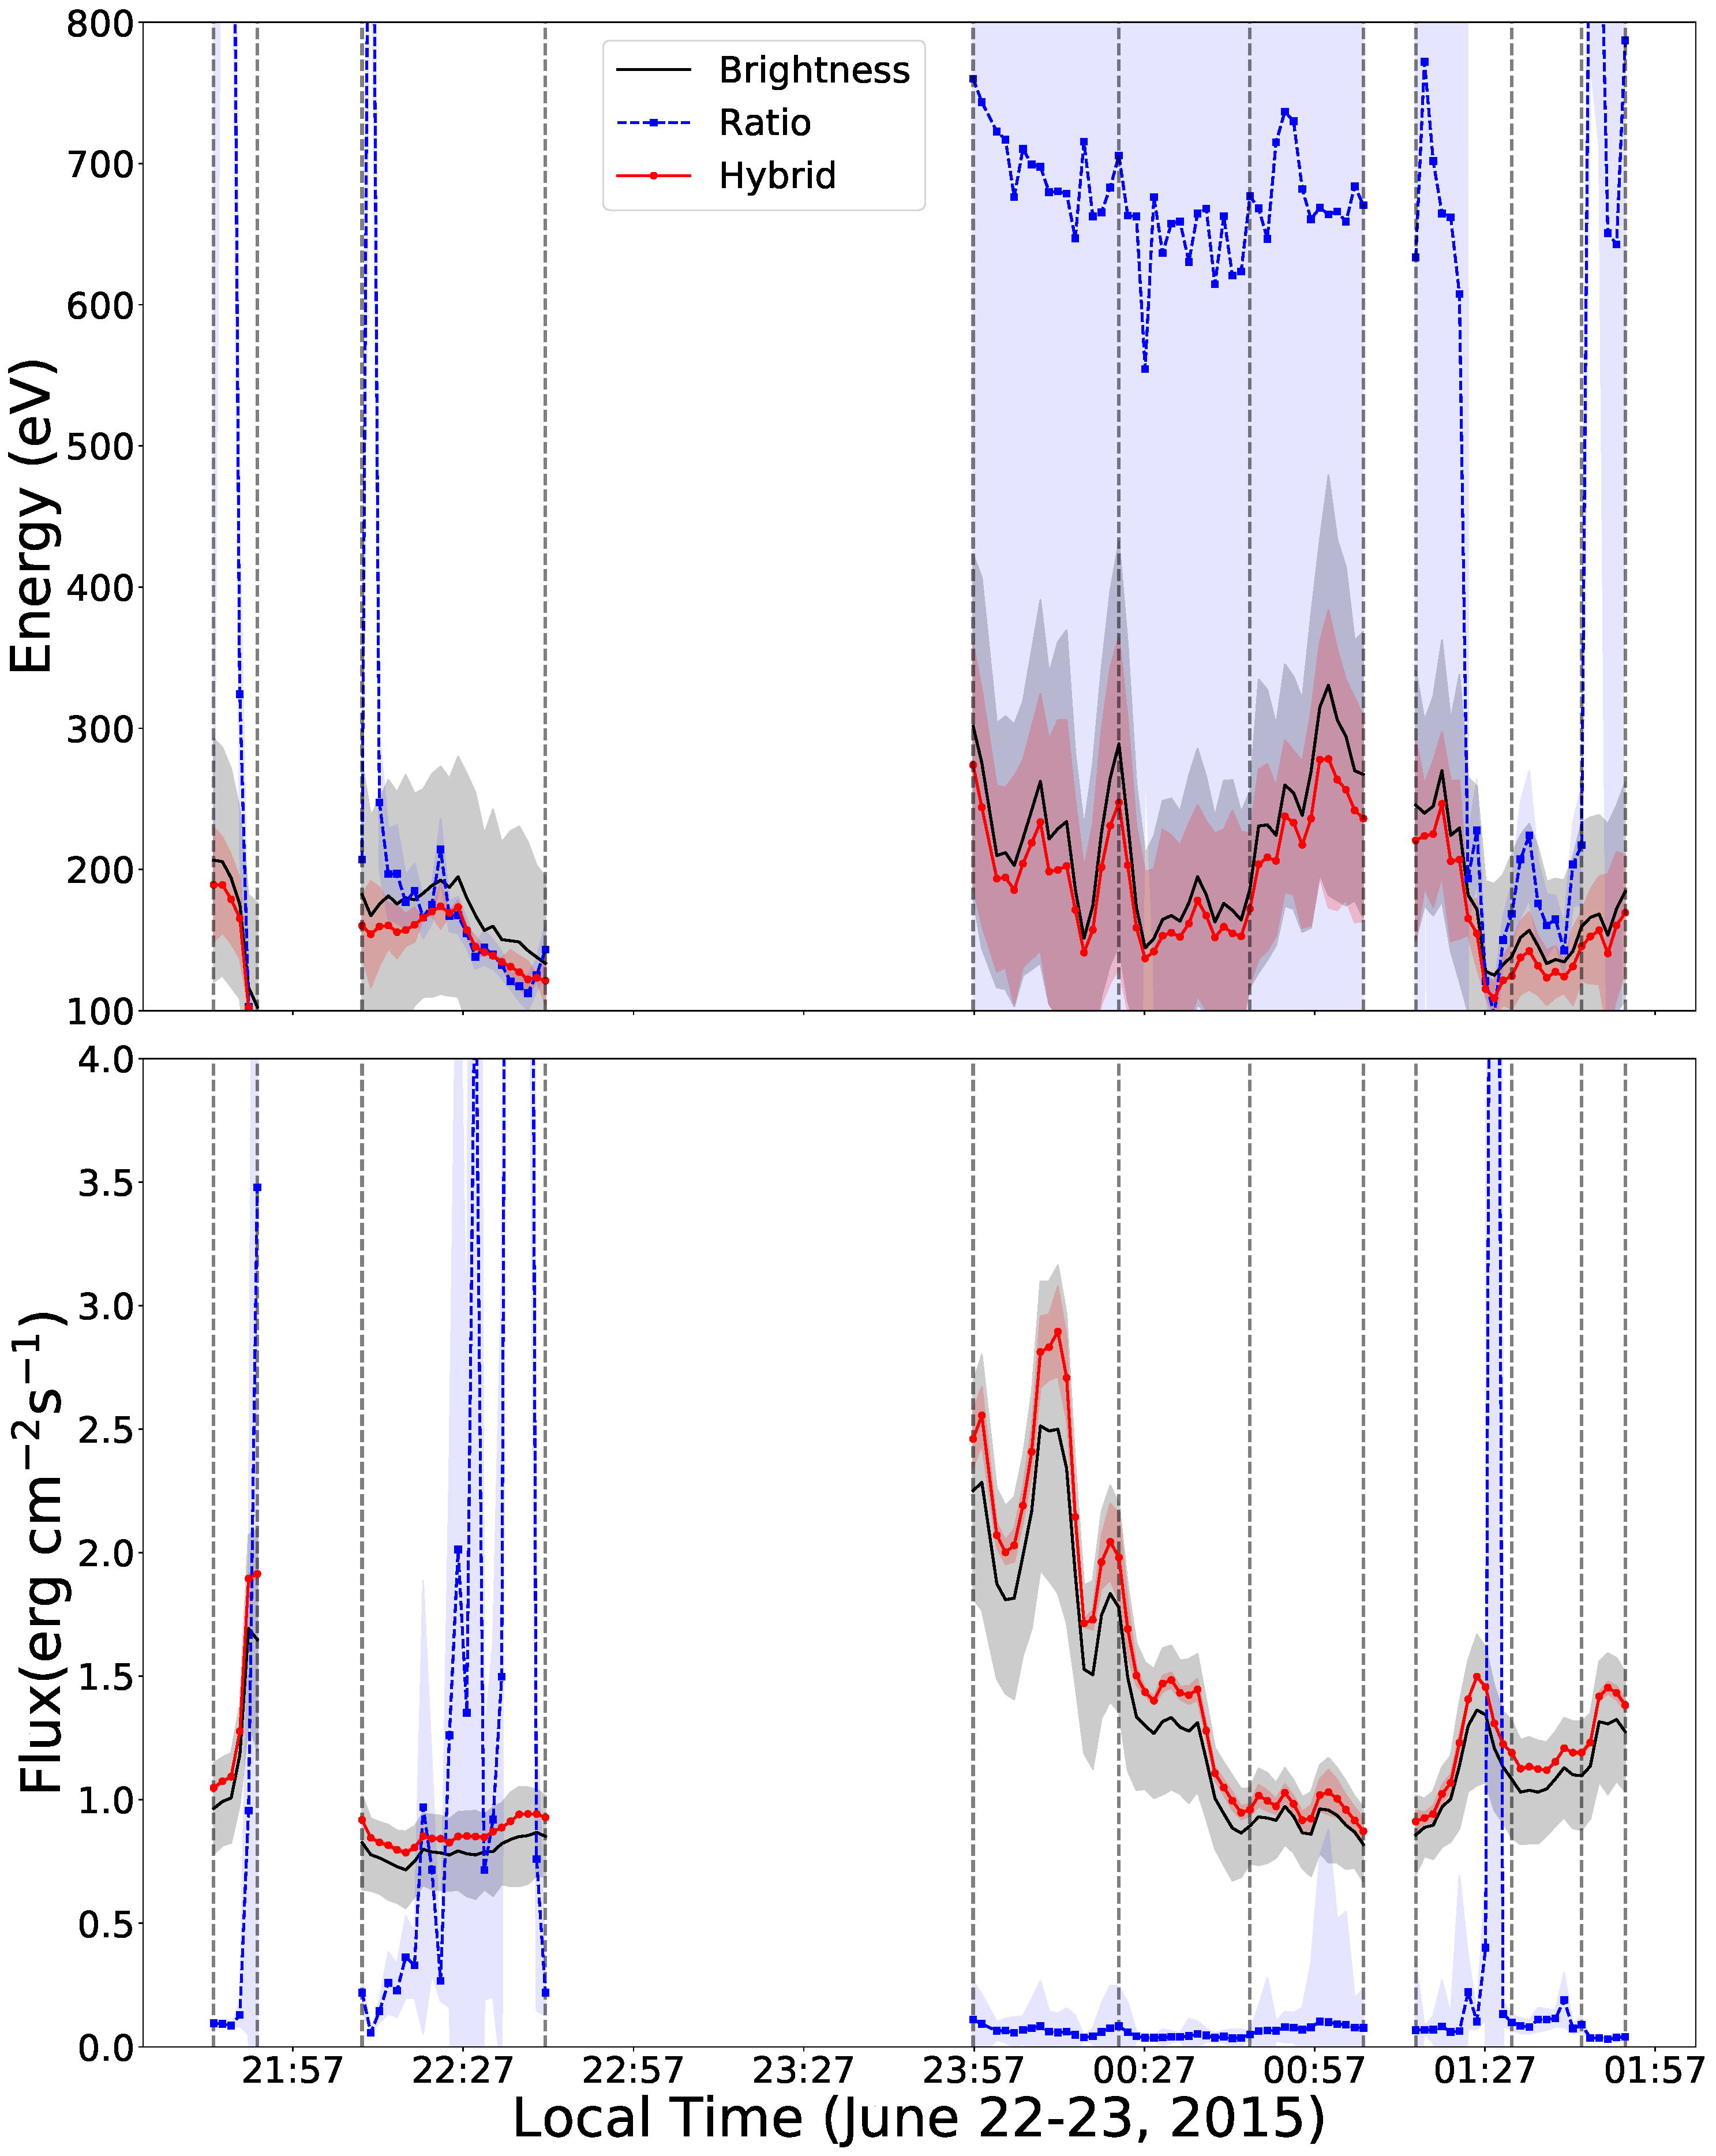
\includegraphics[width=30pc]{different_method_e_fl.pdf}
	\caption{Energies and fluxes derived from 37 to 54$^\circ$ ZA by using three different methods on June 22-23, 2015. Shaded regions denote $\pm$ 1-$\sigma$ statistical uncertainty in the derived results. The brightness and the hybrid methods are in good agreement with each other while for the ratio method, the derived energies and fluxes are inconsistent with the other two methods and the derived uncertainties are significantly larger. Blank areas denote cloudy times based on the NeI 630.5 nm line shown in Figure \ref{feature:nbrg}.}
	\label{fig:e_fl_3mtd}
\end{figure}

The brightness method was initially applied by using all four emission brightnesses. Using the additional OI (777.4 nm) line, however, increased the uncertainties in the derived quantities. Using the red, green and blue lines, the energies and fluxes derived using the brightness method were similar to the hybrid method. This method also produced good match with the measured red and the green line brightnesses when the derived energies and fluxes were set as inputs back into the GLOW model (Figure \ref{fig:e_fl_b_comp}). 

The ratio method had the highest uncertainties in the derived energy and fluxes (Figure \ref{fig:e_fl_3mtd}). The energies and fluxes derived using this method were also not in agreement with the brightness and the hybrid methods. The derived energies for the ratio method ranged from 52 eV to 1200 eV while the flux ranged from 0.08 to 10 erg $\rm cm^{-2} s^{-1}$. In addition, the retrieval of the red and the green line profile with the derived energies and fluxes as input was not accurate (Figure \ref{fig:e_fl_b_comp}). The hybrid method produced the best results but needed a flux to be picked in the first step and the errors in the energy derived in the first step was not propagated to the second step. 

To study why the results obtained from the ratio method differed so significantly from the results of the other two methods, we plotted the $\rm \chi^2$-values from 00:08 and 01:27 LT on June 23, 2015, as a function of characteristic energy and total energy flux. Results from the brightness and ratio methods are shown in Figures \ref{fig:chi_08} and \ref{fig:chi_127} respectively. At 00:08, the energies and fluxes derived using the ratio method are very different from those given by the hybrid and brightness methods, while at 01:27 the energies derived using all three methods are similar. Figures \ref{fig:chi_08} and \ref{fig:chi_127} show that while the brightness method is sensitive to both energy and flux, the ratio method only appears to be sensitive to variations in energy. We speculate that this is because the flux information is lost when the brightness ratios are determined, since all the brightnesses increase with increasing flux. In addition, Figure \ref{fig:chi_08} shows a tightly constrained minimum $\rm \chi^2$ for the brightness method, away from which the $\rm \chi^2$ values rise quickly. However, for the ratio method, shown in Figure \ref{fig:chi_127}, similar $\rm \chi^2$ values are found far away from the minimum, suggesting that the minimization will be more susceptible to systematic errors, including those caused by our viewing geometry. At 00:08 LT (T3 in Figure \ref{feature:nbrg}), we saw an increase in brightness toward the north in the red line emission, while the changes in the blue and green line brightnesses with zenith angle were minimal. Because the red line aurora is visible from farther north compared to blue and green line emissions (Figure \ref{fig:elayer1}), it is possible that we could have been looking at spatially separated features in the red line aurora, which were unrelated to the blue and green line emissions at the same time. If this were true, it would also affect the accuracies of the hybrid and the brightness methods. Indeed, we see that there is larger mismatch between the retrieved blue line brightness at 00:08 LT using the hybrid and the brightness methods compared to 01:27 LT (Figure \ref{fig:e_fl_b_comp}). Furthermore, the lack of sensitivity to average flux could also cause the energies to be derived incorrectly, since the minimization of $\rm \chi^2$ using the ratio method depends on both the energy and flux parameters simultaneously.
\begin{figure}[H]
	\centering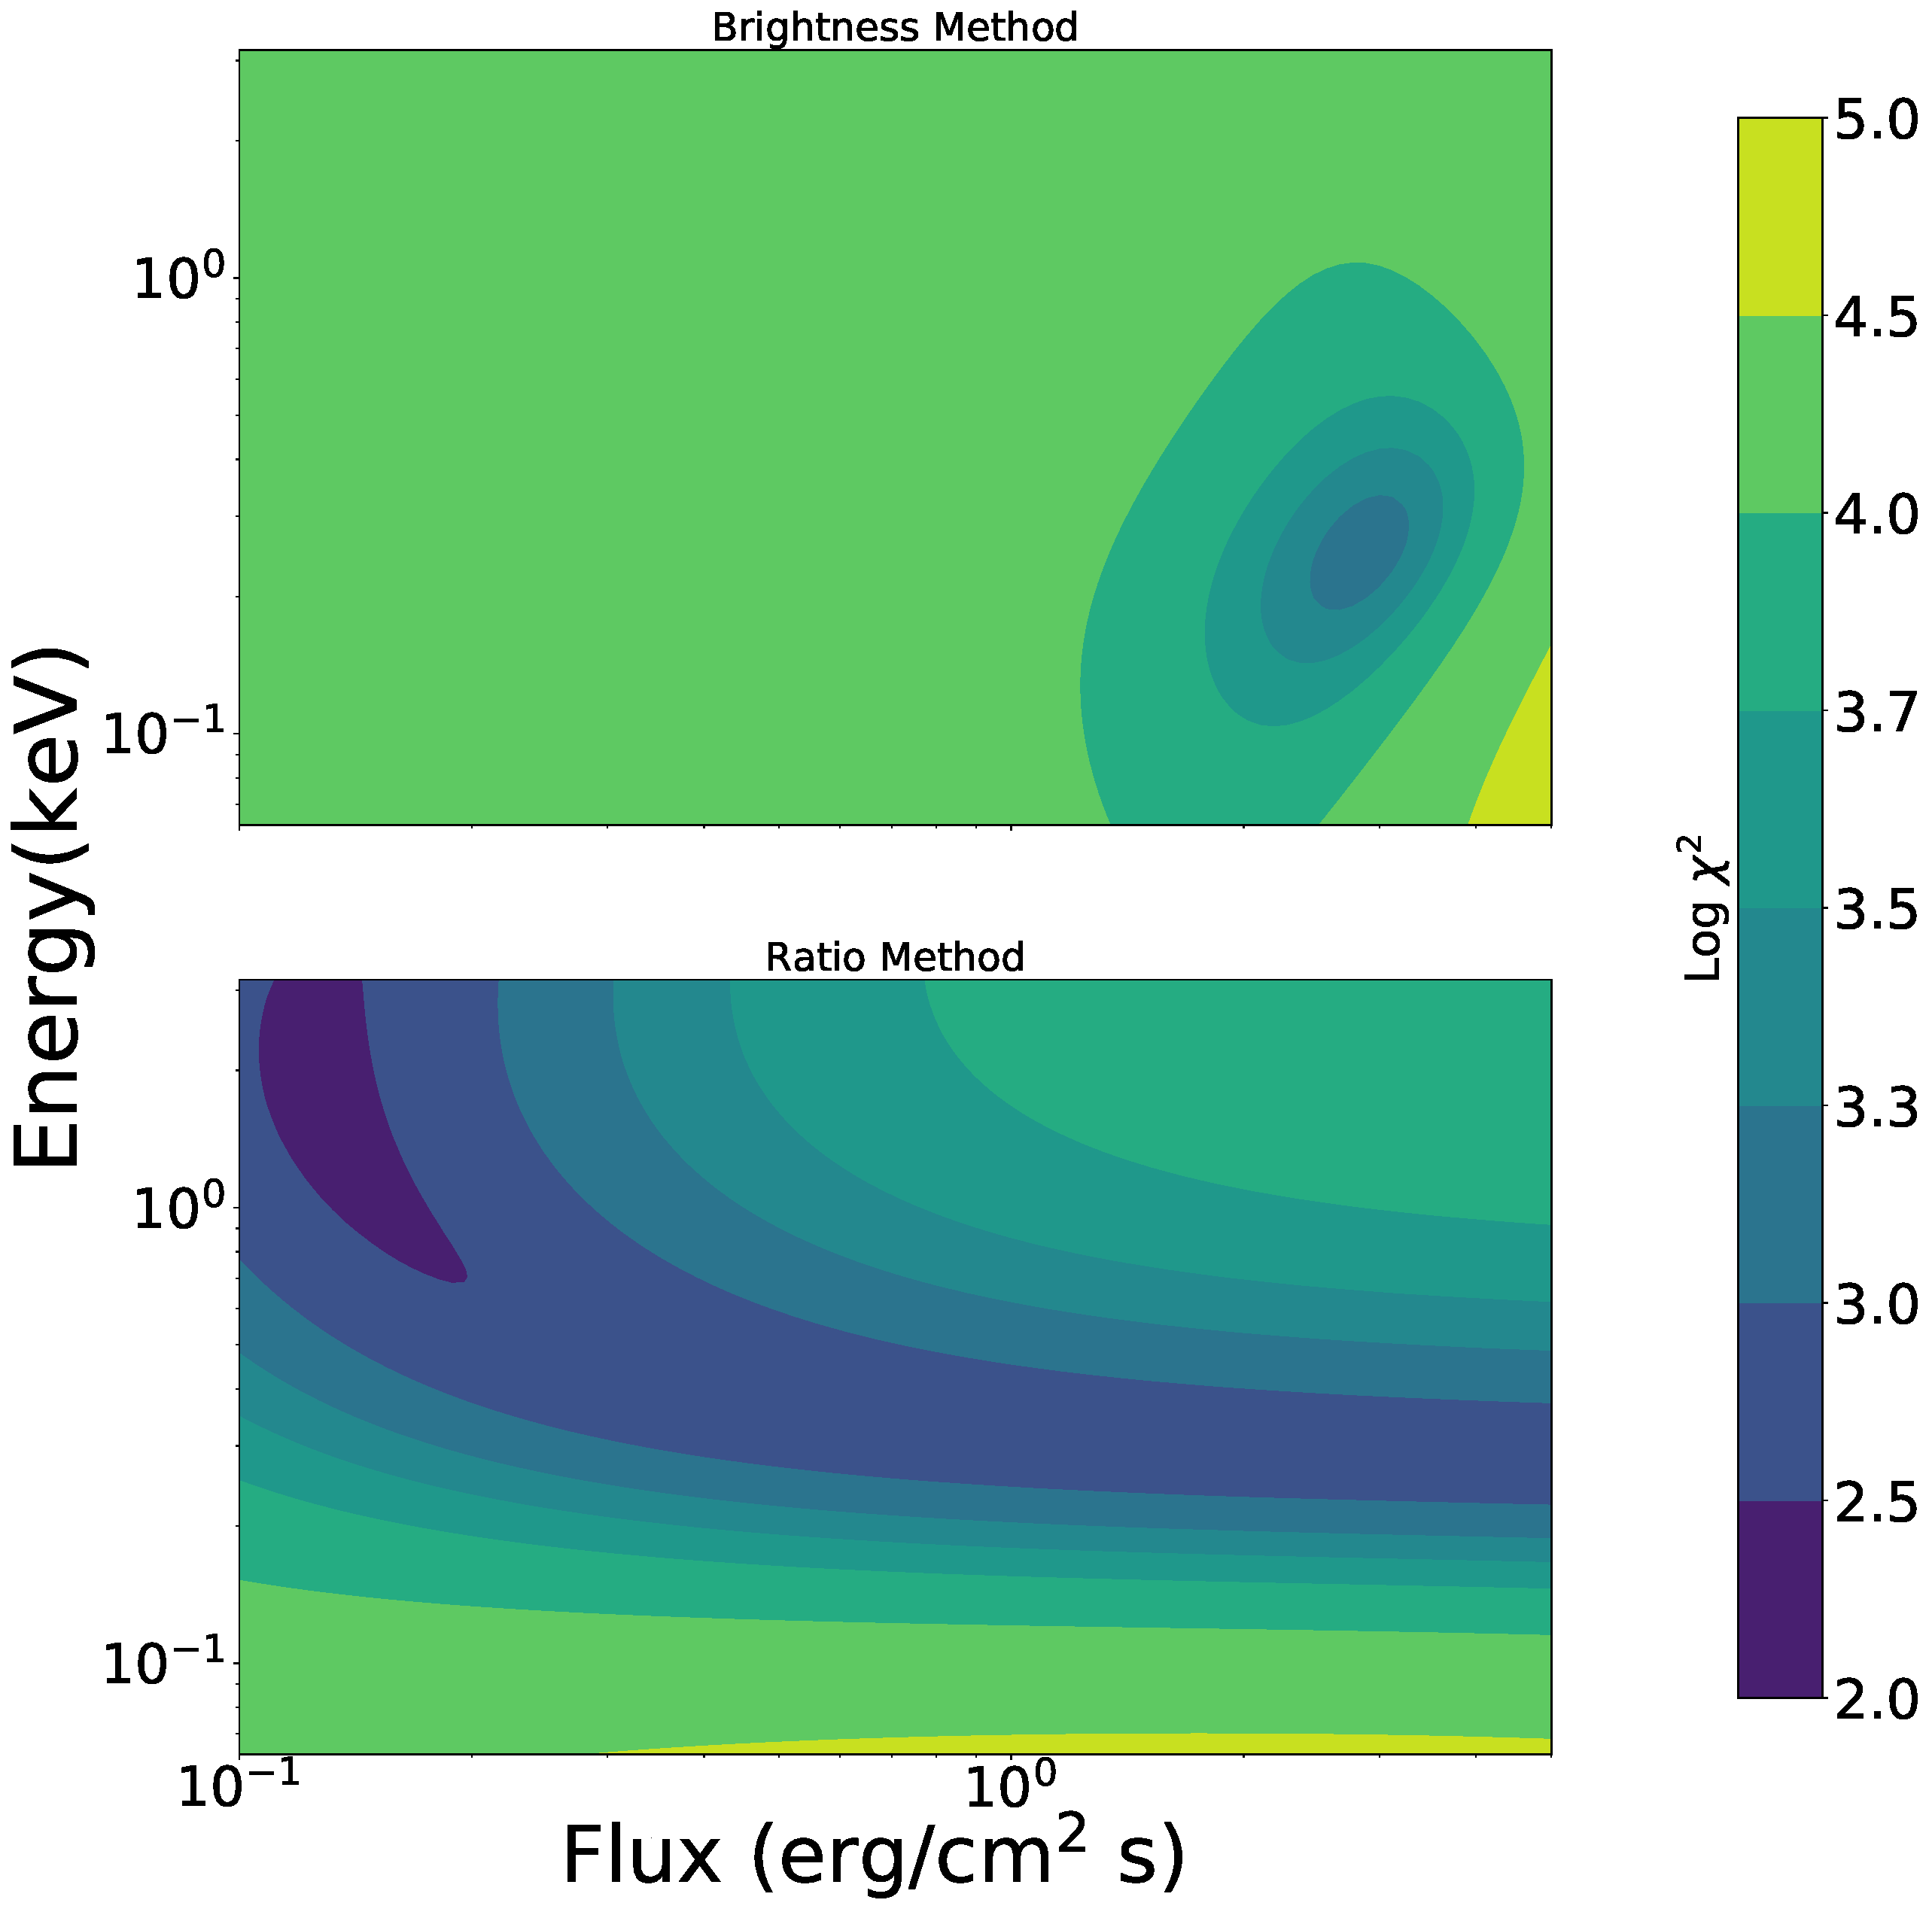
\includegraphics[width=32pc]{chi_b_vs_e_08.pdf}
	\caption{Log $\rm \chi^2$ as a function of characteristic energy and total energy flux at 00:08 LT, June 23,2015 using the brightness method (top) and the ratio method (bottom). Notice that for the brightness method, the minimum $\rm \chi^2$ is well-constrained for both energy and flux parameters.}
	\label{fig:chi_08}
\end{figure}
\begin{figure}[H]
	\centering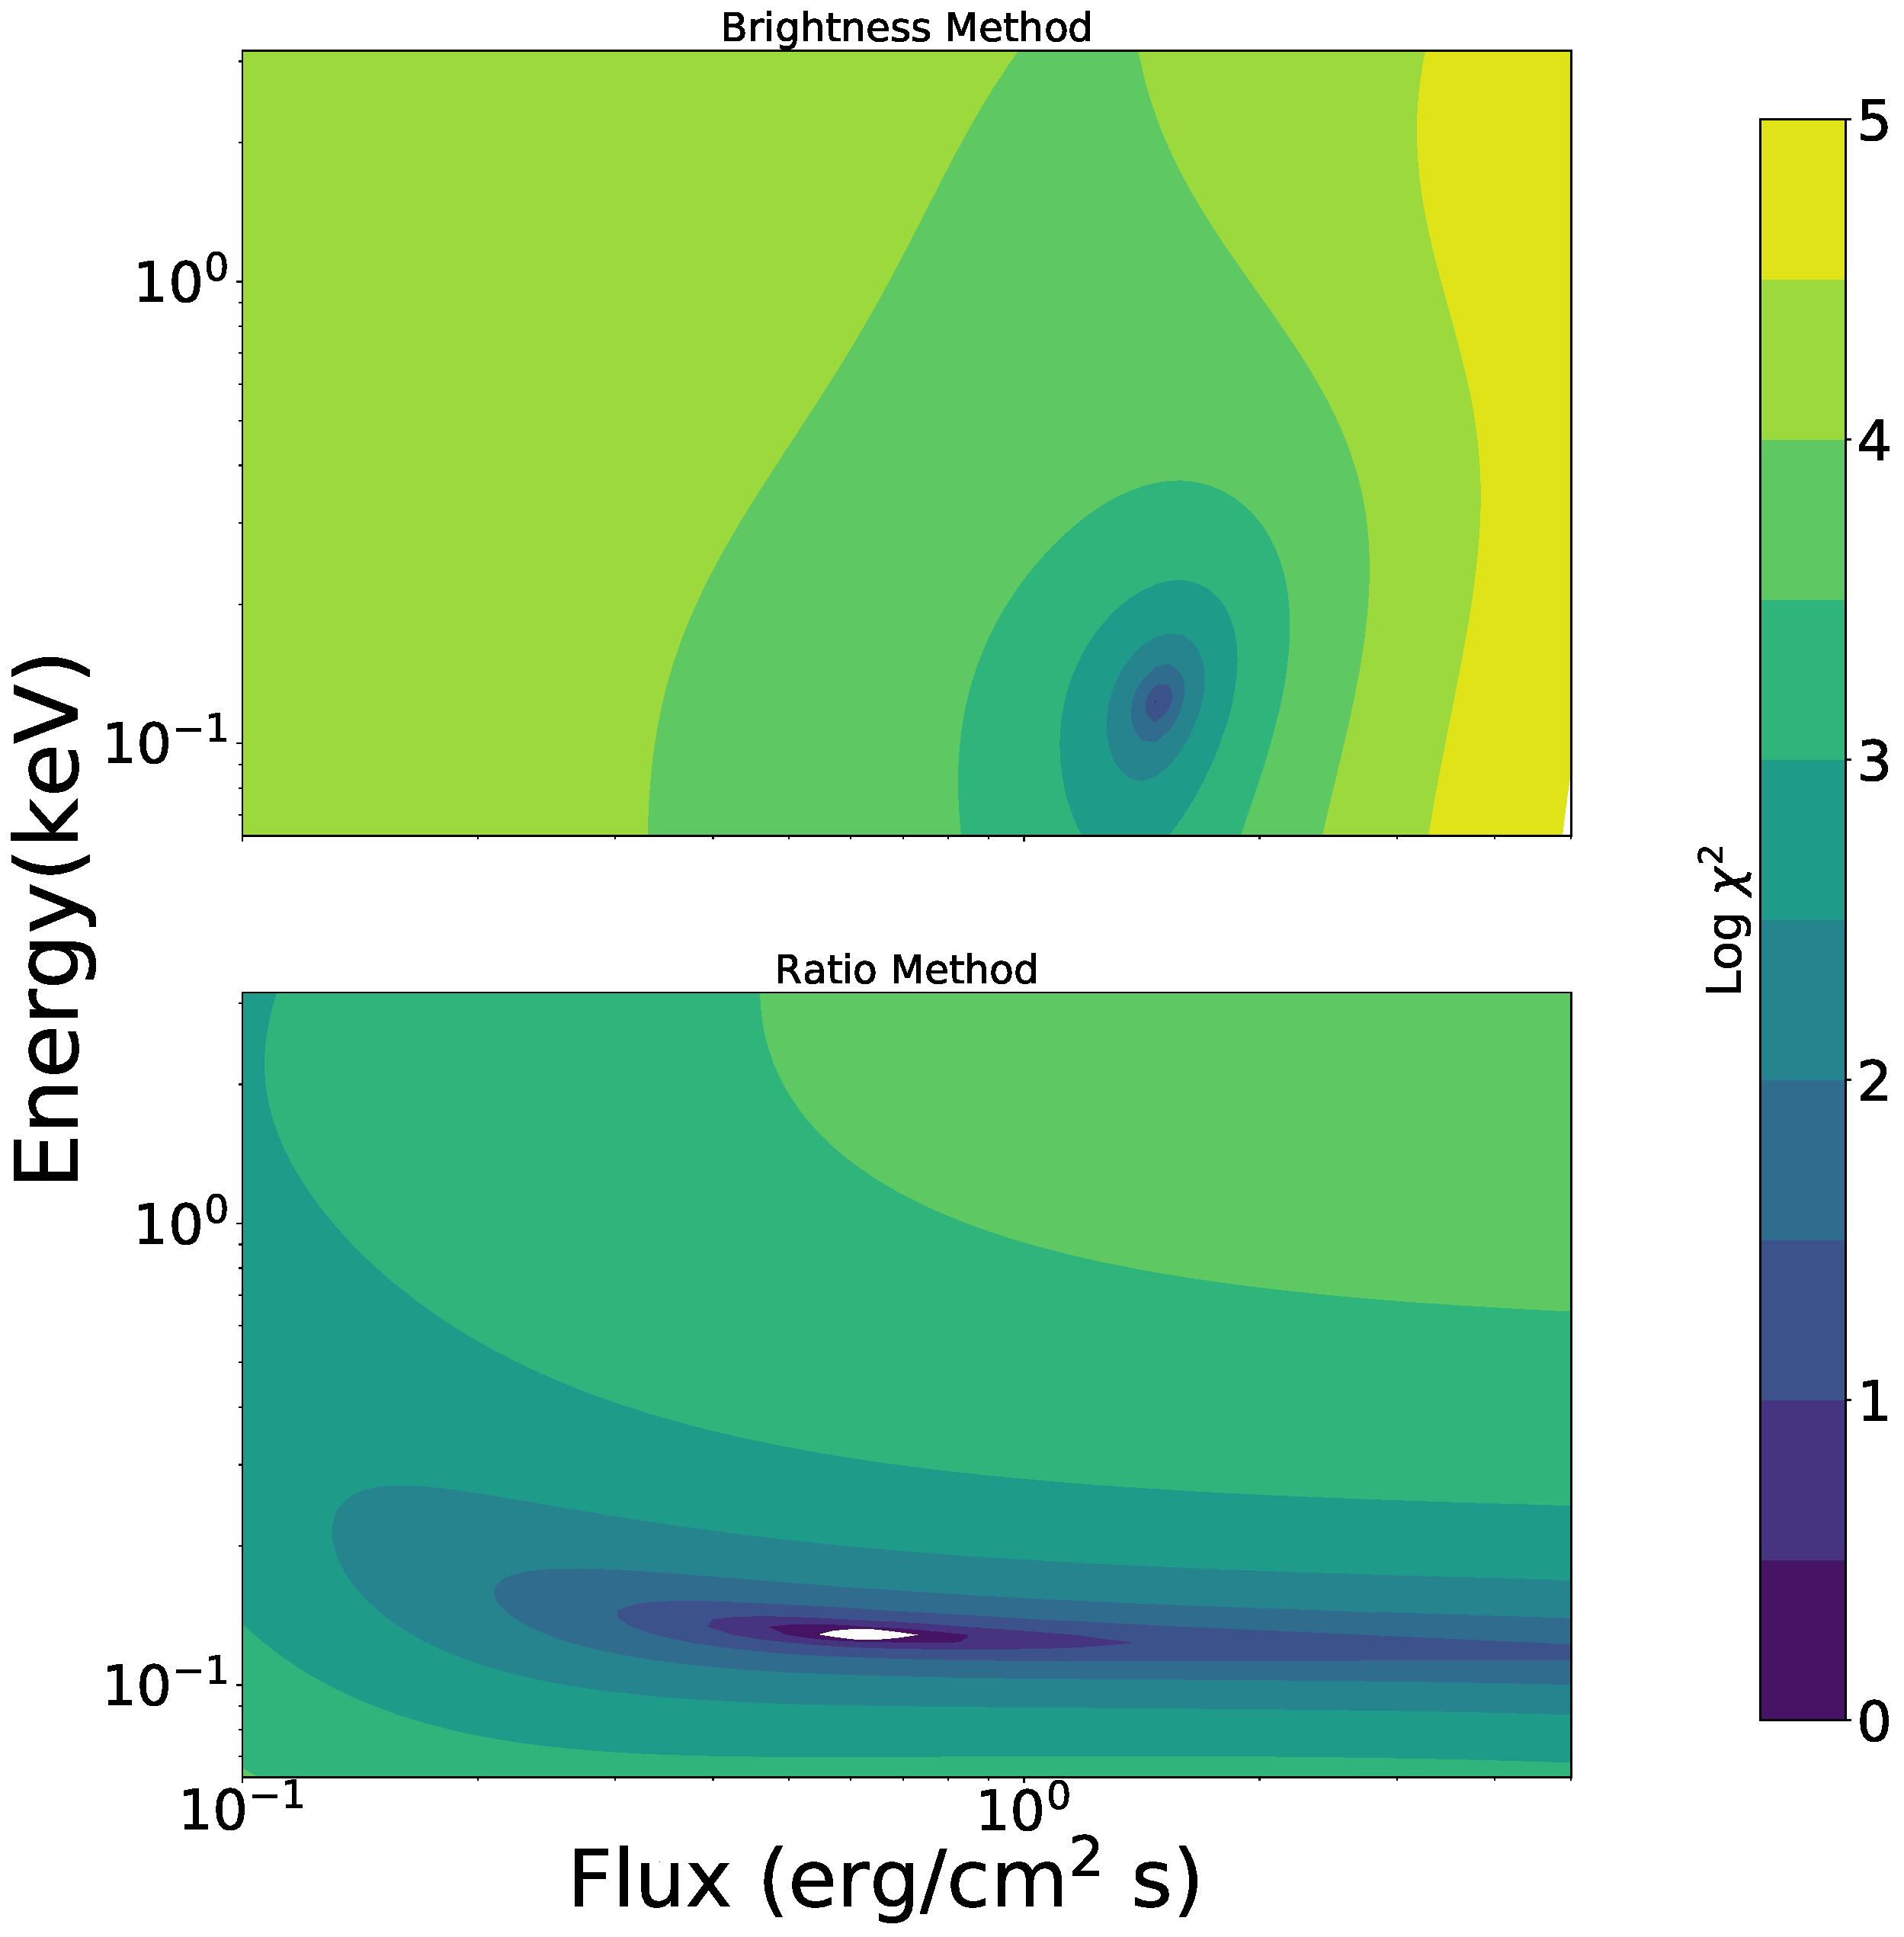
\includegraphics[width=32pc]{chi_b_vs_e_127.pdf}
	\caption{Log $\rm \chi^2$ as a function of characteristic energy and total energy flux at 01:27 LT, June 23,2015 using the brightness method (top) and the ratio method(bottom). Notice for the ratio method, the spread of $\rm \chi^2$ away from the minimum is much smaller than the brightness method.}
	\label{fig:chi_127}
\end{figure}

The hybrid method also uses the brightness ratio in the first step; however, for a fixed flux (1 erg $\rm cm^{-2}s^{-1}$), $\rm \chi^2$ (using brightness ratio) is sensitive to energy (Figure \ref{fig:chi_hybrid}). In the second step, at the energy derived in step one, we minimized $\rm \chi^2$ using brightness to derive fluxes as brightnesses are sensitive to changes in flux.
\begin{figure}[H]
	\centering\includegraphics[width=32pc]{different_fl_evschi2.pdf}
	\caption{Log $\rm \chi^2$ as a function of characteristic energy at a constant flux of 1 erg $\rm cm^{-2} s^{-1}$ at 00:08 and 01:27 LT on June 23. The location of the minimum is used to estimate the energy in the first step of the hybrid method.}
	\label{fig:chi_hybrid}
\end{figure}

The brightness method produced results similar to the hybrid method without requiring an initial guess of $Q_0$. Additionally, the computational time for the brightness method was around 33\% faster using a single core CPU (for 249 data points) compared to the hybrid method. The retrieval of red and green line brightnesses from both hybrid and brightness methods, by using the derived energies and fluxes as inputs to GLOW model, were consistent with the observed brightnesses. The temporal morphology of blue line brightnesses were reconstructed correctly but the brightness values were overestimated (Figure \ref{fig:e_fl_b_comp}). This could be because the MSIS neutral densities are not accurate during storm time \citep{fang_variations_2012}. Furthermore, since all of our measurements are off-zenith, we could be measuring auroras from different locations especially for higher zenith angles (this is true for all three methods).

Results derived using the ratio method, on the other hand, were not in good agreement with the other two methods (Figure \ref{fig:e_fl_3mtd}). Furthermore, the brightnesses retrieved using the ratio method did not match the observed brightness (see Figure \ref{fig:e_fl_b_comp}). We thus conclude that the ratio method may not be a suitable method to derive energies and fluxes during an aurora. Since the hybrid and the brightness methods produce very similar results, only the results derived using the brightness method are shown for the remainder of this paper.
\begin{figure}[H]
	\centering\includegraphics[width=35pc]{different_method_retriv_comp.pdf}
	\caption{Brightnesses retrieved from 37 to 54$^\circ$ ZA by using the derived energies and fluxes as inputs into the GLOW model are compared against measurements. The three different methods are shown with stars (brightness), dot (hybrid), and dashed (ratio) markers. The shaded regions denote the measured brightnesses within the $\pm$ 1-$\sigma$ uncertainty in the measurements which is more noticeable in the blue line data. Notice that the retrieved red and green brightnesses have a good match well with measured red, green line brightnesses for hybrid and the brightness methods but not for the ratio method. Blank areas denote cloudy times based on the NeI 630.5 nm line shown in Figure \ref{feature:nbrg}.}
	\label{fig:e_fl_b_comp}
\end{figure}

The temporally averaged energies and fluxes derived using the brightness method are summarized in Table \ref{table:efl_look}. These results were obtained by deriving energy and flux at each observation time and then averaging over each of the selected time intervals T1 to T8 (shown in Figure \ref{feature:nbrg}). The energy values derived ranged between 109 to 262 eV while the flux values ranged from 0.8 to 2.2 erg $\rm cm^{-2} s^{-1}$.


\subsection{Energy and Flux Morphology}
\label{sec:emorph}
The derived energies and fluxes show both temporal and spatial variations, as seen in Figure \ref{fig:e_fl_la}. The derived energies were lower and the fluxes higher for small zenith angles during most of time period T1. Temporally, there was a sharp drop in energy and increase in flux during this period, especially at 20-37$^\circ$ ZA. These are consistent with red line brightness profile during the period T1 (Figure \ref{feature:nbrg}) where the brightness was higher for small zenith angles and there was a sudden rise in brightness temporally.
%since the red line is more sensitive to lower energies as the emission originates at higher altitudes. %Hence, for time period T1, the red line brightness was also decreasing for higher zenith angles.

Spatially, for most of time periods T3, T4 and T8 the conditions were opposite (compared to the period T1) with higher energies and lower flux at smaller zenith angles. This is consistent with the increase in the red line brightnesses for higher zenith angle during these periods. As discussed in section \ref{sec:bmorph}, for these periods (T3, T4 and T8), the brightness increase in red line for higher zenith angles was sharp but there were no significant brightness changes in other features. The red line emission is visible farther north (and is always north for a given look direction) because of HiT\&MIS's orientation and the emission's occurrence at a higher altitude compared to the other two lines (Figure \ref{fig:elayer1}). So, we could be detecting auroral structure only visible in red line. Hence, the derived energies and fluxes for these time periods should be treated with caution. Also, since the red line covers a larger latitudinal range, we might be observing a gradient in brightness that was not as apparent in blue and green line brightnesses. 

In addition, SAR (Stable Auroral Red) arcs, that are common in the mid-latitude during geomagnetic storms \citep{mendillo_sar}, can cause brightness enhancements only in the red line. The production source of SAR arcs are thermal fluxes from the inner magnetosphere and not electron precipitation (see \cite{mendillo_sar}; \cite{kozyra_1997,rees_1975} and references therein). Boston University (BU) all-sky images (\cite{asi_1993}) from Millstone Hill (approximately 10 miles southwest of Lowell, MA) show SAR arc in red line data towards the south and not close to HiT\&MIS's FOV (Figure \ref{fig:allsky}). SAR arcs can occur along with aurora near the equatorial edge of aurora \citep{ievenko_2008}; however; we do not see any evidence of this by examining all available BU red line all-sky image data during our observation period. Nonetheless, there were time periods when the sky was cloudy over Millstone Hill but clear in the HiT\&MIS FOV. Thus, we do not completely rule out the possibility of SAR arcs being present in our FOV at those times. This could result in derived energies that are lower than the true energies and the fluxes to be higher than the true fluxes. 
\begin{figure}[H]
	\centering\includegraphics[width=35pc]{allsky.pdf}
	\caption{Boston University's all-sky images at Millstone Hill (approximately 10 miles southwest of Lowell, MA) in red and green lines for few selected times on June 22-23,2015. SAR arc was seen in the red line data towards the south (and moving southwards). HiT\&MIS's approximate FOV is shown with a black line on each image.}
	\label{fig:allsky}
\end{figure}

In the time period T2, the increase in the derived energy corresponds to the peaks in the blue line profiles. The fluxes during most of the time period T2 remained relatively constant indicating that the brightness variations were due to increase in the energy of precipitating electrons. The decrease in energy towards the end of the time period T2 was due to the increase in the red line brightness indicating more electrons (higher flux) with slightly less energy precipitated. 

The derived energies are increasing with time during the period T5 while the fluxes are slightly decreasing. The blue and green line brightnesses during the same time period were increasing similarly to the derived energies while the red line brightness was slowly decreasing. Since the green and blue line emissions occur at much lower altitudes (approximately 150 km and 100 km, respectively) than the red line, they are sensitive to higher energy electrons. This indicates that the energies of the precipitating electrons increased with time during the time period T5 causing the blue and green lines to get brighter, despite the slight decrease in flux.

During the time period T6, all the emission brightnesses increased, with the increase in the red line being most prominent than other features. The derived energies show a decreasing trend with time. Since red line brightness is more prominent for lower energies, it makes sense that T6 shows enhanced red line brightness. Due to an increase in flux, the blue and the green lines also increased in brightness. Thus, the temporal and spatial morphologies in derived energies and fluxes are consistent with the brightness morphologies in Figure \ref{feature:nbrg}. 

Derived energies and fluxes (at 37 to 54$^\circ$ zenith angle) using the brightness and the ratio methods were in good agreement with each other within the margin of 1-$\sigma$ uncertainty as seen in Figure \ref{fig:e_fl_3mtd}. The simultaneous ratio method on the other hand, was not in good agreement with the other methods for most time ranges. We inputed these derived energies and fluxes into the GLOW model to compute brightnesses and compare them with the brightness measurements as shown in Figure \ref{fig:e_fl_b_comp}. Again for the brightness and the ratio methods, the retrieved profile showed excellent agreement with the original brightness profiles for the red and the green lines, and fair agreement with the blue line. However, the profiles retrieved using the simultaneous ratio method was not in good agreement with the original profiles. We thus concluded that the simultaneous ratio method, where derivation were done by minimizing brightness ratios using two parameter variation in energy and flux parameters, was not a suitable method to derive energies and fluxes.



\begin{figure}[H]
	\centering\includegraphics[width=30pc]{ratio_method_dfl.pdf}
	\caption{Energies and fluxes derived from 37 to 54$^\circ$ ZA by using different initial input fluxes in the first step using the hybrid methods on June 22-23, 2015. Shaded regions denote $\pm$ 1-$\sigma$ statistical uncertainty in the derived results. Notice that derived energies and fluxes all match well except for the flux of 0.1 erg $\rm cm^{-2} s^{-1}$. Blank areas denote cloudy times based on the NeI 630.5 nm line shown in Figure \ref{feature:nbrg}.}
	\label{fig:fl_d}
\end{figure}


\begin{figure}[H]
	\centering\includegraphics[width=30pc]{different_ld_m1_e_fl.pdf}
	\caption{Derived energies and energy fluxes using the brightness method at different look directions and times. Blank areas denote cloudy times based on the NeI 630.5 nm line shown in Figure \ref{feature:nbrg}. Notice the derived energies and flux show both temporal and zenith angle variations.}
	\label{fig:e_fl_la}
\end{figure}



%The energy derived using the red to blue ratio and the $\chi^2$ minimization methods are comparable during most time period for measurements closest to the zenith. However, 

\begin{sidewaystable}
	\caption{Average (temporal) energies and fluxes derived at the time periods (T1 to T8) and look directions selected in Figure \ref{feature:nbrg} using the brightness method. In this method, $\chi^2$ in Equation \ref{eq:chi} was minimized by constraining the energy ($E$) and the flux ($Q$) parameters simultaneously by comparing model brightness to measurements.}
	\begin{tabular}{|l|l|l|l|l|l|l|}
		\hline
		Times& \multicolumn{3}{c|}{Energy (eV)} & \multicolumn{3}{c|}{Flux (erg $\rm cm^{-2} s^{-1}$)}\\ 
		\hline
		ZA $\rightarrow$& 20$^\circ$-37$^\circ$                  & 37$^\circ$-54$^\circ$                  &54$^\circ$-70$^\circ$                &20$^\circ$-37$^\circ$               &37$^\circ$-54$^\circ$                &54$^\circ$-70$^\circ$               \\	 \hline 
		
		
		T1   &         147$\pm$35 &         170$\pm$40 &      151$\pm$34 &   1.39$\pm$0.19 &   1.22$\pm$0.12 &   1.18$\pm$0.12 \\
		T2   &         135$\pm$16 &         170$\pm$17 &      150$\pm$15 &   0.75$\pm$0.04 &   0.79$\pm$0.04 &   0.87$\pm$0.04 \\
		T3   &         230$\pm$31 &         221$\pm$29 &      150$\pm$22 &   1.64$\pm$0.11 &   2.02$\pm$0.12 &   2.20$\pm$0.14 \\
		T4   &         179$\pm$24 &         181$\pm$24 &      126$\pm$18 &   1.10$\pm$0.07 &   1.24$\pm$0.07 &   1.33$\pm$0.08 \\
		T5   &         237$\pm$26 &         262$\pm$29 &      213$\pm$25 &   0.85$\pm$0.05 &   0.92$\pm$0.05 &   1.02$\pm$0.06 \\
		T6   &         170$\pm$24 &         195$\pm$25 &      164$\pm$22 &   1.09$\pm$0.07 &   1.12$\pm$0.07 &   1.20$\pm$0.07 \\
		T7   &         125$\pm$22 &         142$\pm$24 &      120$\pm$22 &   0.97$\pm$0.07 &   1.07$\pm$0.07 &   1.19$\pm$0.09 \\
		T8   &         200$\pm$40 &         167$\pm$30 &      109$\pm$24 &   1.11$\pm$0.09 &   1.24$\pm$0.10 &   1.42$\pm$0.12 \\
		\hline
	\end{tabular}
	\label{table:efl_look}		
\end{sidewaystable}

%------------------------------------------------





%------------------------------------------------

\section{Discussion}
The Millstone Hill ISR radar was not observing and no ISR generated plasma profiles were available for our observation period. Thus, we used a digisonde \citep{giro} measurements at Westford, MA during our observation period (solid black line in Figure \ref{fig:digi}) for comparison. The F2 peak height obtaned from the digisonde measurements shows a rising hmF2 compared to the same period one day earlier (geomagnetically quiet time, Figure \ref{fig:digi}). This rise in hmF2 can also be caused by changes in either electric field strengths, winds or temperature. However, there is complete loss of radio signal in the digisonde data for most of our auroral observation period (from $\approx$ 22 LT June 22 to 02 LT June 23 in Figure \ref{fig:digi}). This can be attributed to the absorption of radio waves by excess E-region ionization caused by electron precipitation \citep{pallamraju_2011}. We therefore assumed the changes in brightnesses were due to auroral electrons. Additionally, since the low energy electrons are stopped at higher altitudes \citep{rees_1963} the observed rise in
hmF2 compared to the quiet day (Figure \ref{fig:digi}) is consistent with our results indicating that the energies of precipitating electrons were soft ($<$ 600 eV).

%The measurements  suffers from the fact that 
Since the emission features we observed peak at different altitudes, the measurements trace a wider range of magnetic and geographic latitudes with increasing zenith angles for emissions at higher altitudes (Figure \ref{fig:elayer1}). The results for higher zenith angles, therefore, might be less accurate compared to the results at lower zenith angles. Similarly, our observations were also not aligned along the magnetic zenith. So this could limit the accuracy of the results derived for off-magnetic zenith measurements \citep{grubbs_multi_spec}. In addition, IRI90-generated plasma (election and ion) density and plasma temperature profiles could be inaccurate during storm-time \citep{iri_storm}. Similarly, MSIS00 neutral densities during geomagnetic storms can be up to 40\% inaccurate \citep{fang_variations_2012}. This adds uncertainty to the brightness estimates using the GLOW model. In the present study, the uncertainties in the model were not quantified and the uncertainties in energy and energy flux estimates were purely statistical arising from the minimization of $\chi^2$ in Equation \ref{eq:chi}. Hence, the actual uncertainties in the derived energies and fluxes could be much higher than reported in this paper.    


%   \begin{figure}
%  \centering\includegraphics[width=20pc]{rees_r_data.pdf}
%  \caption{OI 630 nm to $N_{2}^+$ 427.8 nm brightness ratio as a function of $N_{2}^+$ 427.8 nm brightness from GLOW model (solid lines) and data (red points) during Auroral period 1 on
%  Figure \ref{fig:fle} for various energies. This plot is similar to the ratio and brightness plots shown in \citet{rees_1974}, but with measurement data added to the plot.}
%  \label{fig:rees_r_d}
%  \end{figure}
%%%%% The GAMBIT plot

\begin{figure}[H]
	\centering\includegraphics[width=30pc]{digi.pdf}
	\caption{ Digisonde measurements of hmF2 during the period of June 22, 2015 20 LT to 5 LT on June 23, 2015 are shown with the solid black line.
		hmF2 during the same time period (20 LT to 5 LT) by the same digisonde on June 21-22, 2015 on a geomagnetically quiet time are shown with the magenta line.
		The  HiT\&MIS observations were conducted between the two dashed vertical lines. Notice that hmF2 rises up before there is a signal loss on June 22-23 while hmF2 is almost constant (around 300 km) on June 21-22. The loss of signal on June 22-23, 2015 might be attributed to ionization caused by electron precipitation while the rise in hmF2 is a possible indicator of soft particle precipitation. 
	}
	\label{fig:digi}
\end{figure}

\section{Summary}
We have used ground-based spectral measurements to derive the energies and energy fluxes of precipitating electrons during an auroral event triggered by a G4 geomagnetic storm over Lowell, MA. Three different methods were compared based on non-linear minimization of $\chi^2$ in Equation \ref{eq:chi}. First, modeled brightnesses were compared with measurements to simultaneously derive energies and fluxes using the brightness method. Then, a similar technique where modeled brightness ratios were constrained with measurements to simultaneously derive the energies and fluxes was applied. Finally, modeled brightness ratios were compared with measurements to derive energies and then model brightnesses were constrained with measurements to derive fluxes using the hybrid method for comparison.  
%Third, energies and fluxes were simultaneously derived by constraining modeled brightness ratios with measured ratios using the one step ratio method. 
Results derived using the hybrid method (similar to methods used in \cite{rees_1974} and \cite{pallamraju_2011}) and the brightness method were in good agreement and reproduced the observed red and green line brightness profiles well. The derived energies ranged from 109 to 262 eV and the  energy fluxes ranged from 0.8 to 2.2 erg $\rm cm^{-2} s^{-1}$.
\end{document}
% \documentclass[crop=false,class=mitthesis,oneside,font=12pt]{standalone}
%----------------------------Preamble-------------------------------%
\usepackage{amsmath}
%\newcommand{\angstrom}{\textup{\AA}}
\usepackage{microtype}
\usepackage{graphicx}
\graphicspath{{./images/}}
%\usepackage{multirow}
\usepackage{rotating}
\usepackage{natbib}
\usepackage{url}
\usepackage{booktabs}
\usepackage{makecell}
\usepackage{graphicx, float}            % Graphics/Images.
\usepackage{pgfplots, tikz}             % Drawing/graphing tools.
\usetikzlibrary{
    calc,                   % Calculating right angles and more.
    angles,                 % Drawing angles within triangles.
    arrows.meta,            % Latex and Stealth arrows.
    quotes,                 % Adding labels to angles.
    positioning,            % Relative positioning of nodes.
    decorations.markings,   % Adding arrows in the middle of a line.
    patterns,
    arrows,
    shapes,
    shapes.geometric,
    cd,
    hobby,
    babel
}                                       % Libraries for tikz.
\pgfplotsset{compat=1.9}                % Version of pgfplots.
\usepackage[]{pdfpages}
% for line numbers comment the next two lines before final submission
\usepackage{lineno}
\linenumbers*[1]
% use fancyhdr, to enable page style stuff (below)
\usepackage{fancyhdr}
\setlength{\headheight}{15.2pt}
\renewcommand{\headrulewidth}{0pt}

\pagestyle{plain}
\usepackage{import}                     % Import external files.
\usepackage[subpreambles=false]{standalone}      % Complileable sub files.
\begin{document}
\chapter{Was the total solar eclipse of August 21, 2017 responsible for the Traveling Ionospheric Disturbances observed in airglow observations ?}
In this chapter, background on AGWs and associated Traveling Ionospheric Disturbances (TIDs) is provided. Specifically the possibility of the total solar eclipse of August 21, 2017 causing the AGWs that were observed by HiT\&MIS eight hours after the eclipse had passed is discussed. 
\section{Background} 

Atmospheric Gravity Waves (AGWs) manifest as Traveling Ionospheric Disturbances (TIDs) via ion-neutral coupling in the Ionosphere-Thermosphere (IT) system \citep{hines_1960}. TIDs are wave-like plasma oscillations in the ionosphere that can be triggered by various processes (including AGWs) and occur at different temporal and spatial scales. TIDs with wavelengths of 100--300~km are classified as Medium Scale TIDs (MSTIDs) and can be caused by various processes, but in general are associated with tropospheric forcing \citep{kelley}. TIDs with wavelengths larger than 1000 km and with time periods greater than one hour are classified as Large Scale TIDs (LSTIDs) \citep{hocke1996review}.

Most LSTIDs propagate from either pole and are associated with magnetic disturbances. Geomagnetic storms cause rapid enhancement of the auroral electrojet that leads to thermospheric heating and expansion \citep{davis_polar_1971,chimonas_atmospheric_1970}. This generates AGWs that propagate toward the equator. The divergence of AGWs in turn generates LSTIDs \citep{prolss_lstid_2000}. LSTIDs that have propagated equatorward and are associated with geomagnetic storms have been observed by previous studies (see \citet{habarulema_storm_tid}, and references therein). For example, based on magnetometer measurements, \citet{habarulema_storm_tid} showed that equatorward TIDs were launched following a southward turning of the Interplanetary Magnetic Field (IMF).

Besides geomagnetic storms, solar eclipses are also known to excite AGWs \citep[e.g.,][]{liu_1998, chimonas1970}, that alter the  IT system~\citep{Lin2018,harding_nightside_eclipse}. \citet{liu_1998} conclude that the ionospheric perturbations that they observed using ionosondes during the total solar eclipse of October 24, 1995 was most likely due to plasma up-flow and down-flow resulting from the cooling and decrease in photo-electron production induced by the eclipse.

\citet{coster_gnss_2017} found signatures of possible mountain waves, using Total Electron Content (TEC) maps, during the August 21, 2017 eclipse. Furthermore, for the same eclipse event, \citet{goncharenko_mh_hill_eclipse} used co-located measurements of digisonde and the Millstone Hill ISR (Westford, MA, $\sim$ 60\% peak obscuration), and observed a fast (20-40~m/s) upward plasma drift above the peak height of the F2 layer, hmF2, immediately following the maximum obscuration. Neutral wind velocity derived from night-time OI 630.0~nm (red line) emission measurements by a Fabry-Perot Interferometer (FPI) in Brazil showed perturbations in neutral winds far from the path of the August 21, 2017 eclipse. Global-scale simulations using a UV obscuration mask that mimicked the August 21, 2017 eclipse's effect on the upper atmosphere successfully predicted the measured changes (using the red line) in neutral wind qualitatively \citep{harding_nightside_eclipse}.

% The 2017 solar eclipse occurred over the continental USA where numerous satellite receiver and ground based instruments were present, leading to abundance of data for studying the effects on the upper atmosphere. Some of the studies have already resulted in observation of unexpected phenomenon. \citet{coster_gnss_2017}, based on Total Electron Content (TEC) measurements, saw enhanced TEC structure along the Rocky mountains as the eclipse passed through them. Based on differential TEC (dTEC) measurement and EUV occultation map, \citet{mrak_eclipse_2018}, found that the large-scale perturbation structure in dTEC immediately following the eclipse mimicked the gradient of the EUV map. This led them to theorize that the perturbation seen in TEC was a directly a consequence of EUV modulation during the eclipse not AGW's.

On August 22, 2017 a sequence of LSTIDs was observed in the northern hemisphere, following a minor geomagnetic storm (minimum Dst index $\sim$-30 nT, peak Auroral Electrojet index $\sim$1000 nT) over North America. The geomagnetic storm followed the eclipse of August 21, 2017 that occurred 8 hours earlier at Carbondale, IL. In this paper, we present a comprehensive LSTID analysis, by virtue of simultaneous measurements by: ground-based spectral imager, Global Positioning System (GPS) differential TEC maps, and ionospheric parameters derived from digisonde. In this chapter, the TID event analysis and characterizing of the TID wave parameters are discussed in detail. The dominant time period in all of these measurements was found to be around 1.5 hours. In addition, our observations are compared to simulations with the Global Ionosphere-Thermosphere Model (GITM) \citep{ridley_global_2006} to examine how the solar eclipse may have affected the observed TIDs.

\section{Measurements}

\subsection{Spectral measurements}

Our observations of the TIDs from Carbondale, IL (Geographic location: 37.7$^\circ$N, 89.2$^\circ$W)  were made using the High Throughput and Multi-slit Imaging Spectrograph (HiT\&MIS) \citep{hitmis}. HiT\&MIS can simultaneously measure six upper atmospheric emission features at high resolution ($\sim$ 0.02~nm/px in red line, for example). The field-of-view (FOV) of HiT\&MIS is approximately 0.1$^\circ$ by 50$^\circ$ and was centered at an elevation angle of 45$^\circ$ looking towards the northwest (Figure \ref{fig:elayer}). The spectral images were recorded at a cadence of 4 minutes using a CCD camera from 2--10~UTC on August 22, 2017. Simultaneous measurements in the red line and OI 557.7 nm (green line) are used for this particular study. 

\begin{figure}[H]
	\centering\includegraphics[width=30pc]{elayer.pdf}
	\caption{Viewing geometry of the HiT\&MIS instrument August 21-22, 2017 at Carbondale,IL. The latitudes traced by the red and green lines are shown assuming the peak emission height of 250 km and 123 km, respectively. Note that for line of sites closer to the zenith (higher elevation angles), the range of latitudes covered by each emission layer is smaller. However for line of sights closer to the horizon (lower elevation angles), emission from a larger latitude range are integrated along the line of sight.}
	\label{fig:elayer1}
\end{figure}

From the raw CCD images, wavelength regions around the red and green lines, plus a diagnostic cloud indicator also observed by HiT\&MIS, were extracted as a function of HiT\&MIS elevation angle and wavelength.  The NeI 630.5 nm line (present in street lights) was used as an indicator of cloud activity as reflection of street lights from clouds acts as a proxy for sky conditions. See Chapter 2 for a more detailed description of the spectra extraction procedure for HiT\&MIS.

For each feature at each time-stamp, the brightness is obtained by co-adding signals from all wavelength bins around $\pm$0.3 nm from the line center. The brightness is then plotted as a function of elevation angle and time. GLobal airglOW (GLOW) \citep{solomon_1988,solomon1989630,bailey2002} model estimates of the Volume Emission Rate (VER, not shown) provides the peak heights of the red (250~km) and green (150~km) lines in the thermosphere. In addition, the green line has another peak in the mesophere region (96~km \citep{yee1987}), the average of the thermospheric and the mesospheric peak heights is assumed to be the peak green line emission height (123~km). Using these emission heights and the viewing geometry of HiT\&MIS, the elevation angles are then converted to the latitude of the emission height projected on the ground. 

\subsection{GPS Differential TEC measurements}
\label{tec}
In order to compare the airglow brightness morphologies in the spectral data, the differential Total Electron Content (DTEC) maps were used. Continuously Operating Reference Stations (CORS, www.ngs.noaa.gov/CORS) and Crustal Dynamics Data Information System (CDDIS, cddis.nasa.gov) publicly available databases with Global Navigation Satellite Systems (GNSS) observation data were used to obtain the DTEC. This accounted for a total of  $\sim$1800 receivers in the continental US. 

To compute the phase-corrected slant TEC estimates, the approach of \cite{Coster1992} is used. The slant TEC were converted to the vertical TEC (vTEC) via a mapping function applied at 300~km altitude \citep{Klobuchar1987}. The background vTEC are then subtracted to obtain DTEC residuals, using variable orders of polynomials \citep{Mrak2018}. The carrier phase based differential approach provides better accuracy up to 0.03~TECu \citep{Coster2012} (1~TECu = 10$^{16}$e$^-$/m$^2$). The DTEC residuals were mapped to a geographical map at an altitude of 300~km and transformed from the naturally irregular spatial grid into a regular grid \citep[e.g.,][]{Azeem2015, Mrak2018} with a resolution of 0.2$^\circ$ $\times$ 0.2$^\circ$ (geographical coordinates). The differential approach and large spatial coverage ($\sim$15,000 spatial data points at a given time) allow one to extract coherent spatial features of tiny amplitudes. The spatial extent and appearance of the coherent perturbations are presented in the form of 2D projections. We extracted the DTEC time series observations for locations aligned with the HiT\&MIS FOV at the assumed altitude. 

\subsection{Digisonde measurements}
\label{digi_m}

An additional insight into the nature of observed TIDs is provided by the Global Ionosphere Radio Observatory (GIRO) \citep{reinisch2011global}, a network of \textit{ionosondes}, high-frequency (HF) bottomside ionosphere sounders. Two GIRO locations operated by Idaho National Laboratory at Idaho Falls, ID (INL, 43.5$^\circ$N, 112$^\circ$W) and by University of Massachusetts Lowell at MIT Haystack Observatory, Millstone Hill (MH, 42.5$^\circ$N, 71.4$^\circ$W) were selected. Both observatories employed the latest Digisonde model DPS4D \citep{reinisch2009new,digisonde.com} in its high-cadence campaign mode, recording the vertical sounding ionograms once a minute. 
% * <temujinparuhang@gmail.com> 2018-10-29T18:26:28.356Z:
% 
% > \citep{reinisch2009new,digisonde.com
% Doest show up as a clickable link. Not sure if it will in the published form
% 
% ^.

Since the first report of the TID phenomenon detected by means of HF radio interferometry \citep{munro1950travelling}, ionosondes have been used as reliable TID detectors with well-established sensitivity to plasma perturbations, as even minute changes of the electron density cause easily detectable variability of the signal propagation path in the ionosphere. For our investigation, time series of the Maximum Usable Frequency (MUF) at a distance of 3000 km (D), MUF(D)F2, a standard ionogram-derived characteristic was used. MUF(D)F2 (referred to as MUF hereafter) is obtained numerically using the shape of the O-wave signal trace extracted from the ionogram (see \citep{davies1989ionospheric} for details) and its change reflects variability in both peak density and height of the F2 layer. This thus enhances the overall sensitivity to plasma perturbations in comparison to individual analysis of the ionospheric characteristics describing density, reflection height, or columnar content of the ionosphere.

\section{Results}

\subsection{Spectral Data}
 The red and green line brightnesses for the night of the eclipse and TID event (August 22, 2017) are presented in Figure \ref{fig:keo_profile}. The brightness data for the night before the eclipse (August 21, 2017) are also shown for comparison. The red and green line brightnesses on the night with the TID event (August 22) show wave-like brightness perturbations, while the perturbations on the night before (August 21) only coincide with the cloud-indicator, especially in the green line.

\begin{figure}[H]
 \centering\includegraphics[width=35pc]{car_Aug2122_both.png}
 \caption{Left column: Brightness keogram of Ne I (cloud indicator, top), green line (middle) and red line (bottom) as a function of look direction (or latitude) on the night of the eclipse (Aug 22). Brighter color represents higher brightness (in arbitrary units).  
 %White-space represents negative values encountered after baseline subtraction. 
Center column: Brightness averaged over the whole field of view (0.1$^\circ$ by 50$^\circ$) for each representative keogram on the left. Notice clear wave-like perturbations seen in both red and green lines on August 22. Right column:  Same as the center panel but on the night before the eclipse (August 21, keogram not shown). The dips in the green line coincides with the increase in the cloud line brightness. There is a sudden drop in the cloud-indicator brightness around 4~UTC on August 22, this is due to nearby stadium light, which was in HiT\&MIS FOV, being switched off. This is not seen in the red line possibly because the wings of the NeI 630.5 nm spectra leaked into the red line (630.0 nm).  The cloud-indicator level on August 22 are around the same level as August 21 even with the stadium light leak, and lower after the stadium light was turned off. }
\label{fig:keo_profile}
\end{figure}

\subsection{DTEC data}
\begin{figure}[htp]
\centering
\includegraphics[width=23pc]{tec_map.png}
\caption{The LSTIDs event as observed by GPS-aided DTEC maps. (a, top) A representative GPS map of TIDs over continental US, at 4:30~UTC. Red 'X' mark denote the location of the HiT\&MIS instrument at Carbondale, Il (37.7$^\circ$N, 89.2$^\circ$W ) . (b, middle) A DTEC keogram elongated along 89.2$^\circ$W longitude. (c, bottom) A DTEC keogram elongated along 37.7$^\circ$N latitude.}
\label{fig:tecmap}
\end{figure}

To validate the wave-like brightness perturbation seen in the spectral data, DTEC maps over the continental USA were used. Figure~\ref{fig:tecmap} shows an example of the GPS-derived DTEC maps and a set of keograms crossing the location of the HiT\&MIS instrument. Figure~\ref{fig:tecmap} (a, top) shows the geographical extent of the large-scale perturbations at 4:30~UTC, when the geomagnetic activity was already in the recovery phase. The LSTIDs are compact and uniform in longitudes west from $\sim$100$^\circ$, whereas eastward they have latitudinal structures. Curiously, this is an approximate line of geomagnetic declination angle 0$^\circ$ that the structures could be associated with. Further, keograms in Figure~\ref{fig:tecmap}b-c show the temporal extent of the LSTIDs in meridional and zonal direction above the HIT\&MIS location. The peak TID activity was observed in the time range between 3 -- 6~UT. Figure \ref{fig:dtec_carb} shows concurrent, co-aligned time series of DTEC and the dynamic part of the red and green line profiles obtained by polynomial de-trending at Carbondale, IL. The perturbations in the DTEC and in the green and red line brightness coincide between 03--06~UTC, which is also the time period when significant large-scale perturbations were observed in the DTEC keogram (Figure \ref{fig:tecmap}). 

\begin{figure}[H]
	\centering\includegraphics[width=35pc]{aug22_dtec_bper.png}
	\caption{DTEC obtained for Carbondale, IL on August 22, 2017 from GPS-derived TEC measurements (solid lines).  Notice stronger perturbations  and better coincidence from 3--6~UTC (compared to the whole profile) with red and the green line profiles shown in dot-dashed and dashed lines, respectively. This time-frame also coincides with the stronger large-scale DTEC perturbation (Figure \ref{fig:tecmap}) and peak enhancement and recovery of the AE index (Figure \ref{fig:gindx}).}
	\label{fig:dtec_carb}
\end{figure}

\subsection{Digisonde MUF data}
GPS TEC measurements suggested large scale nature of the observed plasma waves. To study this further, the digisonde measurements of various ionospheric parameters from far away locations, Millstone Hill (MH) and Idhao National Lab (INL) were looked into. The profiles of foF1, foF2, and MUF are shown in Figure \ref{fig:digi_w} and shows that while the foF1 frequency drops sharp during the time of the eclipse, no clear perturbation structures can be seen. Furthermore, since the F1 layer disappears during the night no night-time foF1 measurements are available. This means no vertical nature of the observed LSTIDs could be studied using digisonde measurements in the current case. As discused in Section \ref{digi_m}, MUF is more sensitive to ionospheric perturbations so only MUF profiles are used for further analysis.

Figure \ref{fig:digi} shows the MUF timelines at MH and INL from 19~UTC on August 21, 2017 to 6~UTC August 22, 2017. The MUF variability is significant at both locations. The perturbations are also seen immediately prior to the start of geomagnetic disturbances (0~UTC on August 22, 2017). These pre-midnight perturbations might be associated with the after-effect of the eclipse, as \citet{goncharenko_mh_hill_eclipse} also reported enhanced plasma density over MH around 21~UTC (August 21) based on radar measurements, which they attributed to the eclipse's after effect. On the other hand, the post-midnight DTEC, brightness and MUF dynamics were more likely associated with the TIDs generated due to an increase in auroral currents as a result of enhanced geomagnetic activity. We expand on this further in the following section.

\begin{figure}[H]
\centering\includegraphics[width=35pc]{digi_muf_21-22.png}
\caption{Digisonde-derived MUF profiles at Idaho National Lab (INL) and Millstone Hill (MH) from 17~UTC August 21 to 6~UTC August 22, 2017. INL was close to the path of the totality and the  99\% peak obscuration time is shown by dashed-vertical black-line. MH was on the path of partial eclipse and the 60\% peak obscuration time is shown in dashed-vertical red-line. HiT\&MIS observation starts around 2~UTC on August 22 (start time shown in vertical solid black line).}
\label{fig:digi}
\end{figure}

\section{What caused the observed TIDs ?}
  To understand the cause of the observed AGWs and TIDs, the geomagnetic conditions were analyzed. Figure \ref{fig:gindx} shows the Dst and the Auroral Electrojet (AE) indices from 18~UTC on August 21 to 10~UTC on August 22, 2017. The Dst  index is a measure of the equatorial ring current strength and is obtained by averaging ground-based measurements of magnetic fields near the equator. The AE index is a measure of the strength of auroral currents and is obtained from magnetic field measurements near the polar cap. The AE strength is directly related to Joule heating of the IT system \citep{ae_joule} which, in turn, could potentially lead to equatorward propagating TIDs (see \citep{kauristie_dst} and references therein for details). 
  
LSTIDs arrived over the FOV at about 1~UTC and lasted until around 6~UTC. Likewise, the AE index began to intensify at approximately the same time, and relaxed back to prior values after 6~UTC. In addition, the keogram shows a complex structuring of the LSTIDs. The leading fronts initially arrived from the north-east and moved towards the south-west (1--4~UTC), but latter were almost perfectly elongated in the zonal direction (4--6~UTC). TIDs in smaller scales within the LSTIDs can also be observed; these are most likely caused wave breaking of the LSTIDs. It is thus concluded that the observed LSTIDs (and AGWs) were most likely generated by geomagnetic effects that induced changes in the auroral current leading to rapid heating and expansion of the thermosphere. Further insight is also gained by looking at the field aligned current measurements (Figure \ref{fig:fac}), which shows enhancement in FACs when compared to the night before..

\begin{figure}[H]
\centering\includegraphics[width=30pc]{tid_geindex.png}
\caption{Dst and AE indices before and during HiT\&MIS observation times. Note the increase in AE starting at midnight UTC on August 22, 2017. }
\label{fig:gindx}
\end{figure}
\begin{figure}[htp]
\centering\includegraphics[width=35pc]{fac.png}
\caption{FAC at 3 UTC on August 21-22, 2017. Notice clear enhancement on August 22. }
\label{fig:fac}
\end{figure}

\section{Wave Characteristics}

Wavelet analyses is performed on the red and green line brightness profiles obtained at Carbondale, IL, digisonde MUF profiles obtained at INL and MH, and the DTEC measurements for Carbondale, IL. Wavelet analysis has been used by previous studies to identify wave characteristics of AGWs and TIDs \citep[e.g.,][]{singh_effect_2016,wvlt_B}. \citet{singh_effect_2016} studied the vertical propagation of AGWs due to a cyclone by performing wavelet analysis on optical emission brightnesses originating at different altitudes. \citet{wvlt_B} used wavelet analysis to study the variation in the geomagnetic field induced by eclipses.
 
The wavelet analysis is based on the guide presented in \citet{torrence_wavelet} and implemented using the Waipy package on Python (\url{https://github.com/mabelcalim/waipy}). Red and green line brightness profiles averaged over the whole FOV were used as there was no significant change in dynamic behavior as a function of elevation angle or latitude (see Figure \ref{fig:keo_profile}). 
The average brightnesses and MUF profiles were subtracted with a polynomial fit in order to remove the long-term climatological trends. The extraction of the dynamic part of the TEC measurement, DTEC, has been described in Section \ref{tec}. These dynamic profiles were then zero-mean, unit variance normalized and the wavelet analysis was performed on these normalized values. Finally, the dominant time periods were obtained from the global wavelet spectra whose Full Width at Half Max (FWHM) was used to estimate the uncertainty.

The wavelet spectra for the red and the green lines, shown in Figure \ref{fig:red_green_wv}, reveal a dominant wave period of 1.3$\pm$0.5 hours for the red line and 1.6$\pm$0.8 hours for the green line. However, the wavelet power for the red line peaked around 2--5~UTC and the green line wavelet power peaked around 3--6~UTC. The DTEC wavelet spectra show a dominant time period of 1.7$\pm$0.7 hours also has a peak around 3--6~UTC (Figure \ref{fig:wav_tec}). The MUF wavelet spectra for both locations show similar dominant wave periods of around 1 hour (and other modes) with peaks at two different times (Figure \ref{fig:muf_wv}). The wave period of 1 hour prior to midnight UTC (at MH) could be the after effect of the eclipse (as discussed earlier) since the perturbations precede geomagnetic disturbances.  
%SM: I changed the narrative a bit. The DTEC spectra is well correlated with green line perturbations, and it peaks 3-6, rather than 4-7. 
%SM: An intriguing discussion can about TEC-green line correlation can be derived based on this observations.

\begin{figure}[H]
\centering\includegraphics[width=35pc]{wavelet_red_green.pdf}
\caption{Left: Wavelet analyses performed on the de-trended red and the green line brightnesses. The dominant wave time period of 1.3 hour and a similar periodicity of 1.6 hour was found for the red and the green lines, respectively. A dashed-black line is shown to highlight the shift in peak time-periods from the red to the green line. The parabolic black line represents represents the cone of influence, below which the results are unreliable. The 95\% confidence-level powers on the wavelet spectra are represented by the dark-purple contour.  Right: The wavelet power spectrum averaged along all observation times and the corresponding Fast Fourier Transform (FFT) power spectrum and wavelet spectrum are shown in gray and black, respectively. The 95$\%$ confidence interval for the global spectra are shown in red. }
\label{fig:red_green_wv}
\end{figure}
\begin{figure}[H]
	\centering\includegraphics[width=30pc]{lomb.png}
	\caption{Lomb-Scargle periodogram for red and green line on August 22, 2017. Notice the peak time periods on both are similar to that obtained using wavelet method.}
	\label{fig:lomg}
\end{figure}
 
\begin{figure}[H]
\centering\includegraphics[width=35pc]{muf_digi_wavelet.pdf}
\caption{Left: Wavelet analysis performed on the dynamic part of the MUF profiles from the MH (top) and  INL (bottom). A dominant time period of 1 hour is seen at both locations at different times after midnight UTC most likely associated with the enhancement in AE. Notice wavelet power spectrum with a dominant time period of 1 hour starting around 21~UTC at Millstone Hill which is before the commencement of a minor geomagnetic storm and could be associated with the after effect of the eclipse. }
\label{fig:muf_wv}
\end{figure}
 
\begin{figure}[H]
\centering\includegraphics[width=35pc]{dtec.pdf}
\caption{Wavelet analysis performed on the DTEC profile at Carbondale, IL from GPS TEC measurements.  The dominant time period of 1.7 hour is seen starting around 4~UTC.}
\label{fig:wav_tec}
\end{figure} 
 
The vertical phase speed was  above the spectrograph was found to be 28~m/s estimated using the time delay obtained by cross-correlation analysis on the dynamic part of the red and green line profiles and the difference in their peak altitude (250 km and 123 km, respectively). The vertical wavelength, $\lambda_z$ =152~km, was calculated using the average of the red and the green line dominant wave time periods (1.4 hours) and the vertical phase speed (30~m/s).  

Maps of DTEC is utilized to estimate horizontal wave parameters. Due to a longitudinal structuring of the LSTIDs,  a latitudinal keogram elongated along 120$^\circ$W is utilized and is shown in Figure~\ref{fig:tec_wave}a. The slope of propagation is found to be 10$^\circ$ per 30~minutes, which translate to meridional speed of 616~m/s, equatorward. Similar estimate can also be found at Carbondale, IL, utilizing keogram in Figure~\ref{fig:tecmap}. Spectral analysis~\citep{Mrak2018gw} was applied to the Keogram~\ref{fig:tec_wave}a, to obtain the dominant meridional wavenumbers. The dominant meridional wavenumber is $\sim$0.005~km$^{-1}$ which translates to meridional wavelength $\lambda_m$=1256~km.

\begin{figure}[H]
\centering\includegraphics[width=35pc]{wl.png}
\caption{LSTID analysis of meridional propagation velocity at 120$^\circ$W (a), and meridional wavelength utilizing 2D FFT analysis (b).}
\label{fig:tec_wave}
\end{figure} 

\section{Effects of the Total Solar Eclipse on the observed LSTIDs}
A total solar eclipse had occurred eight hours earlier before the observed LSTIDs (at Carbondale, IL). While the LSTIDs were most likely generated by geomagnetic effects, the effect of a total solar eclipse on the IT system has also been well-documented by recent and prior studies  \citep[e.g.,][]{coster_gnss_2017,Mrak2018,liu_1998}. Furthermore, the MUF profile at  MH showed perturbations even prior to the start of the geomagnetically active time (Figure \ref{fig:digi}). This could potentially be due to the lingering effect of the eclipse.  
%%% From Ingrid

To test eclipse's effect for our observations, the Global Ionosphere Thermosphere Model (GITM) \citep{ridley_global_2006} was used to simulate the effects of the August 21, 2017 eclipse on the IT system. The Flare Irradiance Spectral Model (FISM; \cite{Chamberlin2007}) was used to specify the solar EUV spectrum, but this was modified to reduce the EUV heating and ionization in the region of the lunar occultation of the Earth to simulate the eclipse effect.
This was done as described by \citet{wu_gitm-data_2018}, although they used a different EUV model. The path of the eclipse was defined in Geocentric Solar Ecliptic (GSE) coordinates as a straight line in the (Y$_{GSE}$, Z$_{GSE}$)-plane, assuming X$_{GSE}$ constant. The reduction in EUV irradiance was based on the distance between each GITM grid point and the center of totality; at the center of totality, the EUV irradiance was reduced to 10\% of the normal value, which linearly increased until the edge of the occultation region was approached, after which the EUV increased exponentially back to 100\% at 3,800 km distance from the center of totality.
% * <temujinparuhang@gmail.com> 2018-10-02T19:30:55.601Z:
% 
% > This was done as described by \citet{wu_gitm-data_2018}, although they used a different EUV model.
% Any reference to what the EUV model used?
% 
% ^ <icnossen@googlemail.com> 2018-10-09T12:04:34.743Z:
% 
% I've added this to the text. The full reference is:
% ^ <temujinparuhang@gmail.com> 2018-10-29T15:49:10.678Z.

%
% ^.
Two simulations were run; one with the eclipse event included, and, one without for comparison (the control simulation). Both simulations were otherwise set up identically. The model was run with a resolution of 2.0$^\circ$ in latitude, 4.0$^\circ$ in longitude, and $\sim$0.3 times the scale height in altitude, spanning from 100 km to approximately 600 km altitude. Observed solar wind and interplanetary magnetic field data were used to drive the high-latitude electric potential and auroral precipitation patterns. The simulations used here are the same as those analyzed by Cnossen et al. [in preparation], who describe the simulation setup in further detail. 
   \begin{figure}[H]
 \centering\includegraphics[width=35pc]{ec_vs_nec_tid.pdf}
 \centering\includegraphics[width=30pc]{GITM_with_GLOW_dglow.pdf}
 \caption{ Electron densities  and the thermospheric O/N$_2$ ratio at 250 km (peak of red line emission) using an EUV mask to mimic the effect of a total solar eclipse, and no-eclipse conditions (but including geomagnetic effects) using the GITM model at Carbondale, IL. Notice that while the profiles are very similar, both electron density and the O/N$_2$ ratios are $\sim$ 10\% higher when the effects due the eclipse were considered. }
 \label{fig:ec_ne}
 \end{figure}
 
 %%%%%
 
   \begin{figure}[H]
 %\centering\includegraphics[width=35pc]{ec_vs_nec_tid.pdf}
 \centering\includegraphics[width=30pc]{GITM_with_GLOW_dglow.png}
 \caption{ Electron densities  and the thermospheric O/N$_2$ ratio at 250 km (peak of red line emission) using an EUV mask to mimic the effect of a total solar eclipse, and no-eclipse conditions (but including geomagnetic effects) using the GITM model at Carbondale, IL. Notice that while the profiles are very similar, both electron density and the O/N$_2$ ratios are $\sim$ 10\% higher when the effects due the eclipse were considered. }
 \label{fig:glow_est}
 \end{figure}
 
% * <icnossen@googlemail.com> 2018-09-24T11:26:01.141Z:
% 
% > To test this further the Global Ionosphere Thermosphere Model (GITM) \citep{ridley_global_2006} was used to simulate the effects of the August 21, 2017 eclipse on the IT system. To do this, GITM was modified to reduce the EUV heating and ionization in the region of the moon occultation of the Earth. This was done as described by \citet{wu_gitm-data_2018}, although they used a different EUV model. The path of the eclipse was defined in Geocentric Solar Ecliptic (GSE) coordinates as a straight line in the (Y$_{GSE}$, Z$_{GSE}$)-plane, assuming X$_{GSE}$ constant. The reduction in EUV irradiance was based on the distance between each GITM grid point and the center of totality: at the center of totality, the EUV irradiance was reduced to 10\% of the normal value, which linearly increased until the edge of the occultation region was approached, after which the EUV increased exponentially back to 100\% at 3,800 km distance from the center of totality.
% > Two simulations were run: one with the eclipse event included and one without for comparison (the control simulation). Both simulations were otherwise set up identically. The model was run with a resolution of 0.5$^\circ$ in latitude, 2.0$^\circ$ in longitude, and $\sim$0.3 times the scale height in altitude, spanning from 100 km to approximately 600 km altitude. Observed solar wind and interplanetary magnetic field data were used to drive the high-latitude electric potential and auroral precipitation patterns. The simulations used here are the same as those analyzed by Cnossen et al. [in preparation], who describe the simulation setup in further detail. 
% This is a methodology description, so you could consider making a separate section for this, before presenting the results. This could be a separate "model simulations" section on the same level as the "data" section, or you could make a "methodology" section, with subsections for the different data sources and the model simulation description. It's up to you, but I think it works better to keep the methodology separate from the actual results.
% 
% ^ <temujinparuhang@gmail.com> 2018-10-03T23:54:23.973Z:
% 
% I have made a separate section for it but not sure if the title represents that, open to title name suggestions
%
% ^ <icnossen@googlemail.com> 2018-10-09T12:51:10.324Z:
% 
% I think the organization could work this way and the title is fine by me.
%
% ^ <temujinparuhang@gmail.com> 2018-10-29T15:49:20.142Z.
% The electron transport model, GLOW \citep{solomon_1988,solomon1989630,bailey2002}, was used to estimate the red and green line brightnesses based on climatological and GITM derived inputs. 
%%%%%%%%%%%%%

Figure \ref{fig:ec_ne} shows the electron density and  the thermospheric O/N$_2$ ratios estimated using GITM at 250 km, which is where the red line emission peaks, for the two cases: with and without the effect of the eclipse. Both the electron density and the O/N$_2$ ratio were around 10\% higher when the the eclipse's effect were included but the time profile was very similar to the non-eclipse case.  While these simulation results imply that the eclipse enhanced the TID strength, no conclusion on the possibility of the eclipse contributing to the formation of the observed TIDs could be drawn.  
% * <icnossen@googlemail.com> 2018-10-09T12:52:00.533Z:
% 
% > However, no conclusion on the possibility of the eclipse contributing to the formation of the observed TIDs could be drawn.  
% This seems to contradict your last key point, although I realize that "contributing to the formation" is different from enhancing wave amplitudes. In any case, I think this last point should only follow after a bit more explanation/discussion. 
% I've been thinking a bit more about the resolution of the model versus the scale of the wavelike perturbations you observed. This is when I realized I made a mistake in the model description: the resolution of the model results I gave you was not 0.5 degree in latitude by 2.0 degree in longitude, but 2 degree in latitude and 4 degree in longitude - I have corrected this in the text above. I'm really sorry about this, but it does offer a possible explanation as to why the model is not seeing the wavelike perturbations you observed.  A resolution of 4 degrees in longitude near Carbondale is about 350 km and 2 degrees in latitude is about 220 km. Therefore the model is unlikely to see a wave with a horizontal wavelength of 550 km. Also the vertical resolution of the model is around 10 km at 250 km altitude, and at 150 km altitude the vertical resolution is about 6-7 km, which is better, but still not enough to be able to simulate wavelike perturbations with a 10 km vertical wavelength.
% I do have a set of simulations available at 1 degree latitude by 2 degree longitude resolution which used a slightly different setup.  We could use those instead, but it would mean repeating a bit of analysis and it is still questionable whether the resolution will be good enough (the resolution in altitude is still the same).
% 
% ^ <temujinparuhang@gmail.com> 2018-10-29T23:21:40.297Z:
% 
% "However, no conclusion on the possibility of the eclipse contributing to the formation of the observed TIDs could be drawn. " I have reworded it, hopefully is less confusing now 
% 
% For the resolution part, the calculation of the vertical wavelength was not correct (10 km), it is around 150 km, so I have mentioned lack of latitudinal and longitudinal resolution as the probable reason that we dont see wave-like feature in GITM simulation.
% 
% ^.
 Figure \ref{fig:ec_ne} (bottom) shows GLOW model brightness estimates using GITM inputs (both with and without eclipse's effect). The red and the green line brightnesses scaled to the climatological GLOW estimates the night before (assumed to have no disturbances) plus the climatological GLOW brightness estimates are also shown for comparison. GLOW's brightness estimates for the red line using GITM's inputs  with eclipse's effect are comparable to the data until the brightness perturbations occur ($\sim$ 0300 UTC). 
%%%%GITM model e(nhanced Ne
   

%This section describes the GITM model based on writeup I will get from  Dr. Cnossen.
%  Numbered lines in equations:
%  To add line numbers to lines in equations,
%  \begin{linenomath*}
%  \begin{equation}
%  \end{equation}
%  \end{linenomath*}

\section{Discussion}
The dynamic part of the red and green lines and the DTEC profiles at Carbondale, IL, coincided better from 3--6~UTC (August 22, 2017, Figure \ref{fig:dtec_carb} ), which is also when the DTEC keogram show prominent LSTIDs (Figure \ref{fig:tecmap}, bottom). All of the wavelet spectra have a similar dominant wave power around the same time frame (3--6 UTC). In addition, the AE index peaks and recovers during the same time period too (Figure \ref{fig:gindx}). This indicates that the increase in auroral currents and associated Joule heating near the poles were responsible for the observed LSTIDs. There are TIDs prior to and after 3--6 UTC in the DTEC map (Figure \ref{fig:tecmap}, bottom); however, their scale are sizes smaller and and the strength is weaker. 

The estimated dominant wave time-periods are slightly different for different observations, i.e., 1.3$\pm$0.5, 1.6$\pm$0.8 and 1.7$\pm$0.7 h for the red line, green line and DTEC, respectively at Carbondale, IL. The dominant wave period of around 1h was also found for MUF profiles at both INL and MH. MUF is sensitive to the bottom-side ionospheric plasma densities, the red and green line brightnesses are sensitive to both the plasma and the neutral densities at the altitude they peak at, and the TEC measurements are sensitive to the line of sight ionospheric plasma density. These differences could explain the discrepancy in dominant time periods. 

Previous studies have observed disturbances in the IT system well after the eclipse and far away from its path \citep[e.g,][]{harding_nightside_eclipse,eclipse_belg}. \citet{goncharenko_mh_hill_eclipse} reported enhanced electron density (> 50-150\%) starting from 21~UTC, August 21, 2017 to at least midnight UTC (August 22) based on radar measurements at MH hours after the eclipse.  The authors attributed this enhancement in electron density to the downward flux of plasma from the plasmasphere that was filled by upwelling of plasma immediately following the eclipse. This electron density enhancement was not predicted by GITM, as it does not include contributions from the plasmasphere. 21--22~UTC is also when one of the peaks in MUF wavelet spectrum with a dominant wave time-period of around 1h at MH is observed (Figure \ref{fig:muf_wv} ). This indicates that the observed perturbation in MUF was caused by eclipse related effect with similar time period of around 1h that was observed later with the geomagnetic effect. \citet{wu_gitm-data_2018} reported that the IT system's response to the eclipse in GITM decays much quicker than is seen in TEC and NmF2 observations. On the other hand, a 10\% increase in both O/N$_2$ ratio and N$_e$ at Carbondale, IL predicted by GITM is consistent with the quantitative enhancement in the observed red line brightness observed when compared to the night before (see Figure\ref{fig:supp} ). However, GITM failed to produce the wave-like perturbations seen red and green line airglow brightnesses, possibly due coarser resolution in latitude and longitude. Thus, it is possible that eclipse's long-term effect not only influenced the TID strength, but also could have interacted with the geomagnetic effects in the formation of the observed LSTIDs. Based on this study it can only be concluded that the eclipse's effect only enhanced the TID's strength. 
% * <temujinparuhang@gmail.com> 2018-10-29T23:33:09.191Z:
% 
% > However, GITM failed to produce the wave-like perturbations seen red and green line airglow brightnesses, possibly due coarser resolution in latitude and longitude
% Might have to re-word this open to suggestion
% 
% ^.
% * <icnossen@googlemail.com> 2018-10-09T13:54:40.491Z:
% 
% > ; however, no conclusion on that could be drawn based on this study
% In that case it should not be listed as a key point.
% 
% ^ <temujinparuhang@gmail.com> 2018-10-29T23:23:56.232Z:
% 
% Re worded this part to make it sound in non-formal terms : "the eclipse influnced the TID strength, but we dont know if the eclipse induced pre-conditioning helped in the formation of the TID"
%
% ^.

  \begin{figure}[H]
 \centering\includegraphics[width=35pc]{supplimentary1.pdf}
 %\centering\includegraphics[width=30pc]{GITM_with_GLOW_dglow.pdf}
 \caption{ Red line brightnesses (in arbitrary units) on August 21-22, 2017. Notice around 10\% enhancement on August 22 when compared to August 21.}
 \label{fig:supp}
 \end{figure}
 
Multi-spectral observation from HiT\&MIS would have been sufficient to infer the vertical wave characteristics of the TID; but the brightness perturbation spanned its FOV, so the meridional scale-size of the TID could not have been estimated. Similarly, using the DTEC measurements meridional wave characteristics could have been estimated, but not the vertical wave characteristics. Utilizing multi-instrument observations we were able to characterize the wave properties, and infer that geomagnetic disturbance-induced Joule heating was the most likely source of these TIDs.
% * <icnossen@googlemail.com> 2018-10-09T13:58:57.420Z:
% 
% > predicted geomagnetic disturbance-induced joule heating to be the source as well as characterize the wave properties. 
% This part of the sentence does not work gramatically and I don't think you "predicted" anything. I think you might want to say something like: ", characterize the wave properties, and infer that geomagnetic disturbance-induced Joule heating was the most likely source of these TIDs."
% 
% ^ <temujinparuhang@gmail.com> 2018-10-29T23:29:12.970Z:
% 
% changed as you suggested
%
% ^.
% * <icnossen@googlemail.com> 2018-10-09T13:55:44.893Z:
% 
% > Multi-spectral observation from HiT\&MIS would have been sufficient to infer the vertical wave characteristics of the TID; but the brightness perturbation spanned its FOV, so the scale-size of the TID could not have been estimated.
% I don't understand this. I'm probably confused by what you mean with "scale-size". Does that refer to the horizontal direction?
% 
% ^ <temujinparuhang@gmail.com> 2018-10-29T21:01:02.813Z:
% 
% yes, replaced with "meridional scale size"
%
% ^.
% * <temujinparuhang@gmail.com> 2018-10-04T21:21:06.076Z:
% 
% > Utilizing multi-instrument observations we were able to establish the large-scale nature of the observed TIDs, predicted geomagnetic disturbance induced joule heating to be the source as well as characterize the wave properties. 
% I think we need one more line here to end this section.. open to suggestions
% 
% ^.

% SM: TIDs are becoming a very popular topic. I miss a part where you conclude a narrative into a closed story. At this point, there are observations and a brief discussion. Here you have a place to put the observations into a broader context. What is the contribution of the HIS imager? Are there any know studies of LSTIDs utilizing ground-based imagers of spectrographs? What new contributions do you show with combining 3 remote observation techniques and a model output? What can differences in peak period, and time delay between different observations tell us about the physical processes (you made some comments already there)? etc... 
% * <icnossen@googlemail.com> 2018-09-24T11:35:28.866Z:
% 
% > SM: TIDs are becoming a very popular topic. I miss a part where you conclude a narrative into a closed story. At this point, there are observations and a brief discussion. Here you have a place to put the observations into a broader context. What is the contribution of the HIS imager? Are there any know studies of LSTIDs utilizing ground-based imagers of spectrographs? What new contributions do you show with combining 3 remote observation techniques and a model output? What can differences in peak period, and time delay between different observations tell us about the physical processes (you made some comments already there)? etc... 
% I agree!
% 
% ^ <temujinparuhang@gmail.com> 2018-10-29T21:02:42.450Z.

\section{Summary}
Analysis of wave-like perturbations observed in red and green line brightness from ground-based optical measurements was presented. Additional insight was provided by MUF profiles based on digisonde measurements and GPS-based TEC measurements. Using wavelet analyses, all of the measurements show a similar dominant time period of about 1.5 hours. We conclude that a geomagnetic disturbance starting at midnight UTC on August 22, 2017 enhanced the auroral currents that lead to Joule heating which triggered AGWs and associated LSTIDs propagating towards the equator. Furthermore, a total solar eclipse had occurred hours earlier over the continental USA (8 hours earlier in Carbondale, IL). By using the GITM simulation, we found that preconditioning of the IT system due to eclipse increased N$_e$ and O/N$_2$ ratio at 250~km around 10\% during the observed TID event. Using cross-correlation on the red and the green line brightness profiles, the vertical phase speed was found to be 30~m/s. Similarly, spectral analysis of DTEC keogram was used to estimate the meridional phase speed of 616 m/s.
\end{document}
% \chapter{Discussion}

	
\section{Conclusions}


\section{Recommendations} \label{sec:recommendations}


\section{Future Work}


%% This defines the bibliography file (main.bib) and the bibliography style.
%% If you want to create a bibliography file by hand, change the contents of
%% this file to a `thebibliography' environment.  For more information 
%% see section 4.3 of the LaTeX manual.
\bibliographystyle{abbrvnat-quote}
%\bibliographystyle{plainnat}
\renewcommand{\bibname}{References}
\bibliography{Energetics,agusample}

\appendix
%\include{appendix-stub} 	%I used an appendix stub file before I wrote the real appendix so the main file would build correctly.
%% Sherman v1
\chapter{If you need an Appendix}

If you need a appendices, make them here, as chapters. You can copy this file so each appendix has its own tex file, in which case you need to add them to main.tex. Or, you can put them all in this one file. 

%\chapter{Author Biography}

As of 2012, UMass Lowell calls for a ``Biographical Sketch of Author.''

The required brief biographical sketch should include the names of schools attended, the exact designation of diplomas and degrees awarded, the title and nature of any post-collegiate employment, together with the name and location of the employing organization, and a description of any previous graduate study or related research, publications, or special professional interests.


\end{document}
